% Bronbestand (bevroren 2026-09-20). Eerder gegenereerd door
% dutch/tools/make-book-master.py (nu gearchiveerd in dutch/attic/);
% bewerken gebeurt direct in dit bestand en de dutch/*.tex-hoofdstukken.
\def\printmanual{true}
\documentclass{book}
\usepackage[dutch,shorthands=off]{babel}

% Dutch babel definieert enkele kapittelnamen via \babelshorthand{"y}
% (de ij-ligatuur), wat mislukt wanneer shorthands=off is. Overschrijf die
% namen met gewone Nederlandse tekst om dat te omzeilen.
\addto\captionsdutch{%
  \def\appendixname{Bijlage}%
  \def\listfigurename{Lijst van figuren}%
  \def\listtablename{Lijst van tabellen}%
  \def\enclname{Bijlage(n)}%
  \def\proofname{Bewijs}%
  \def\glossaryname{Verklarende woordenlijst}%
}

\usepackage[quiet]{fontspec}
\usepackage[table,xcdraw,dvipsnames]{xcolor} % Used by spritegrid and others.
\usepackage[obeyspaces,spaces]{url}
\usepackage{longtable}
\usepackage{arydshln}
\usepackage{booktabs}
\usepackage{afterpage}
\usepackage{flushend}
\usepackage{titletoc}
\usepackage[toc]{appendix}
\usepackage{parskip}
\usepackage{graphicx,wrapfig}
\usepackage{float}
\usepackage{caption}
\usepackage{pdfpages}
\usepackage{tikzpagenodes}
\usepackage{imakeidx}
\usepackage[pagestyles,raggedright]{titlesec}
\usepackage[all]{nowidow}
\usepackage{etoolbox}
\usepackage{alphalph}
\usepackage{datetime}
\newdateformat{dateyear}{\THEYEAR}

% Change the hyperanchors to allow more than 26 appendices
\appto\appendix{
  \renewcommand\thechapter{\AlphAlph{\value{chapter}}}%
}

\usepackage[bookmarks=true,linktoc=all]{hyperref}

\usepackage{tabularx}

% NB: de kolomtypes L/R hieronder gebruiken \raggedright. Dat zet
% \rightskip op 0pt plus 1fil, waardoor regelafbreking nooit "druk" heeft om
% een woord te splitsen: in smalle omschrijvingskolommen (de IEC-tabellen
% gebruiken L{6cm}) levert dat grote gaten aan witruimte en ongebroken lange
% Nederlandse woorden ("verzending"). Daarom zetten we de rekbaarheid van
% \rightskip daarna terug op een eindige 2em, zodat afbreken weer mogelijk
% wordt. Dit is wat ragged2e's \RaggedRight ook doet, maar zonder package:
% \RaggedRight blijkt niet te combineren met de cellen die \newline gebruiken
% (dat levert "Missing } inserted" op). De Engelse common-header.tex gebruikt
% nog de kale \raggedright, dus de pagina-indeling loopt iets uiteen.
\hypersetup{
  colorlinks   = true, %Colours links instead of ugly boxes
  urlcolor     = blue, %Colour for external hyperlinks
  % Each main .tex file configures via \titleformat the \chapter command
  % to do {\chapmtoc\insertminitoc} and \chapmtoc, as defined below, will
  % use \hypersetup{linkcolor=white} to avoid blue-on-blue TOC links
  % Besides, each main .tex file will issue the \tableofcontents command
  % between \hypersetup{linkcolor=black} and \hypersetup{linkcolor=blue}
  % This means however that if "blue" is modified here it must be modified
  % in these files too.
  linkcolor    = blue, %Colour of internal links
  citecolor   = red %Colour of citations
}
\usepackage{aeb-minitoc}
\usepackage{fix-cm}
\usepackage{textpos}
\usepackage{enumitem}
\usepackage{tcolorbox}
\tcbuselibrary{breakable,listings,skins,xparse}
%\usepackage{wrapfig}
\usepackage{needspace}
\usepackage{verbatim}
\usepackage{ean13isbn}
\usepackage{setspace}

% Use CHAPTER-PAGE page numbering to make it easier to modify chapters
% later, without messing up page number of the rest of the book.
\usepackage[auto]{chappg}

% Allow cross-references between the various books to the big The MEGA65 Book
\usepackage{xr}
\usepackage{varioref}
% Nederlandse vertaling van varioref-referentieteksten
\renewcommand{\reftextfaraway}[1]{op bladzijde~\pageref{#1}}
\renewcommand{\reftextpagerange}[2]{op bladzijden~\pageref{#1}--\pageref{#2}}
\renewcommand{\reftextlabelrange}[2]{\ref{#1} tot~\ref{#2}}
\usepackage{xparse}

\usepackage{colortbl}
\usepackage{adjustbox}

% Deelboeken verwijzen naar de Nederlandse titels van het grote boek; die
% staan in de aux van de build met jobname mega65-book-build (dutch/tools/
% build-book.sh mega65-book). Bestaat die nog niet, dan valt het terug op de
% Engelse aux van de Makefile-build. Herbouw na wijzigingen aan het grote
% boek eerst het grote boek, anders staan de titels/paginanummers verouderd
% in de deelboeken.
\IfFileExists{mega65-book-build.aux}%
  {\externaldocument[M65Book-]{mega65-book-build}}%
  {\externaldocument[M65Book-]{mega65-book}}
% And a \ref alternative that checks if it needs to be a cross-reference to the
% MEGA65 Book instead.
\makeatletter
\newcommand{\bookref}[1]{%
    \@ifundefined{r@#1}{%
      {\em het grote Mega65-boek}, \nameref{M65Book-#1} (\autoref{M65Book-#1})}{\autoref{#1}}%
}
\newcommand{\bookvref}[1]{%
    \@ifundefined{r@#1}{%
      {\em het grote Mega65-boek}, \nameref{M65Book-#1} (\autoref{M65Book-#1})}{Hoofdstuk/Bijlage \vref{#1}}%
}
\makeatother

% For fixed-width columns in register maps
\usepackage{array}

% Makes tables with double-ruled lines look better
\usepackage{hhline}

% Makes better use of space for reference tables in appendix
\usepackage{multicol}

% Shaded tables with alternate rows colored for better legibility
% Best used with larger tables rather than small tables
\usepackage{colortbl}
\usepackage{adjustbox}
\usepackage[strict]{changepage}

% \makecell command for forcing line breaks in table cells
\usepackage{makecell}

\newcolumntype{L}[1]{>{\raggedright\rightskip=0pt plus 2em\relax\let\newline\\\arraybackslash\hspace{0pt}}m{#1}}
\newcolumntype{C}[1]{>{\centering\let\newline\\\arraybackslash\hspace{0pt}}m{#1}}
\newcolumntype{R}[1]{>{\raggedleft\let\newline\\\arraybackslash\hspace{0pt}}m{#1}}

% clear to left page for making two page tables starting on the odd page
\newcommand{\cleartoleftpage}{%
  \clearpage
  \ifodd\value{page}\hbox{}\newpage\fi
}

% Layout structures for acknowledgements pages
\newenvironment{mega65thanks}{
    \setlength{\linewidth}{125mm}
    \setlength{\columnsep}{3mm}
    \begin{multicols}{2}
}{
    \end{multicols}
}


% For displaying Letter keys and the MEGA key
% This is a `keys' element for displaying a Mega65 keyboard key
% using a black filled label with rounded edges.
% In order to display a key as a title, use:
%
%     \megakey[title]{Run/Stop}
%
% For displaying a key as a part of the normal document flow, simply use:
%
%    \megakey{Shift}
% 
% Other sizes are supported, as part of tcolorbox: http://mirror.aarnet.edu.au/pub/CTAN/macros/latex/contrib/tcolorbox/tcolorbox.pdf#subsubsection.4.7.5 however, only `title' and the default: `small' are proposed for use in this manual.

\usepackage{tcolorbox}
\usepackage[utf8]{inputenc}

\newtcbox{\megakey}[1][small]{colback=black, coltext=white, size=#1, fontupper=\bfseries\uppercase,nobeforeafter,box align=bottom,text height=7pt}


% For displaying print versions petscii character symbols
% This is a collection of symbol macros element for displaying a printed version of the
% MEGA65 graphic characters, as opposed to the bitmap versions in the mega40/80.ttf fonts files.
% You can display characters using the graphicsymbol macro:
%
%    \graphicsymbol{\textcolor{red}{qQ} wWUcbdhjI \textcolor{blue}{JK}}
%
% Or you can, simply use the font itself:
%
%    \begin{symbolfont}%
%	   qQwWeErRtTyYuUiIoOpP\\
%		 aAsSdDfFgGhHjJkKlL\\
%		 zZxXcCvVbBnNmM%
%		 \end{symbolfont}%
%
%
% You can display the MEGA symbol using:
%
%    \megasymbol
%
% This will display the symbol in black. Other colours can be specified by passing them in, for example:
%
% 	 \megasymbol[black]
%		 \megasymbol[white]
%		 \megasymbol[orange]
%		 \megasymbol[blue]
%
% NOTE:
% For using the MEGA symbol in a key, see the \megasymbolkey macro in the keys.txt file.

\usepackage{tcolorbox}

\newcommand{\graphicsymbol}[1]{%
\begin{symbolfont}%
#1
\end{symbolfont}%
}%

\newcommand{\megasymbol}[1][black]{%
\begin{symbolfont}%
\textcolor{#1}{`}%
\end{symbolfont}%
\
}%


% For Mega65 display of code, listings and screen activity
% This is a collection of elements for displaying output from the Mega65 screen.
% They can display program code or fragments to show activity on the screen.
% Example of use:
%
%    \begin{screencode}
%    10 OPEN 1,8,0,"$0:*,P,R
%    20 : IF DS THEN PRINT DS$: GOTO 100
%    30 GET#1,X$,X$
%    40 DO
%    50 : GET#1,X$,X$: IF ST THEN EXIT
%    60 : GET#1,BL$,BH$
%    70 : LINE INPUT#1, F$
%    80 : PRINT LEFT$(F$,18)
%    90 LOOP
%    100 CLOSE 1
%
%    RUN
%    \end{screencode}
%
% for inline display of code, use:
%
%    \screentext{?SYNTAX ERROR}
%

\usepackage{listings,color}

\lstnewenvironment{screenoutputlined}
   {
     \lstset{
               basicstyle=\codefont\color{white}\linespread{1.0}\normalsize,
               backgroundcolor=\color{black},fillcolor=\color{black},
               rulecolor=\color{black},
               frame=lines,
               framexleftmargin=2mm,
               framexrightmargin=2mm,
               framextopmargin=2mm,
               framexbottommargin=2mm,
               tabsize=4,
               xleftmargin=2mm,
               xrightmargin=2mm,
               basewidth={0.4em},
               literate={\*}{*}1{\-}{-}1{\/}{/}1{{\ }}{{ }}1
            }
   }
   {  }

\lstdefinestyle{megalisting}{basicstyle=\codefont\normalsize,breaklines=false,fontadjust=true,basewidth=1.5mm}

% The heart glyph lives at U+01B3 in the code fonts.  listings only knows
% ASCII (32--127) and Latin-1 (extendedchars), so it does not recognize
% U+01B3: the character is typeset immediately while surrounding characters
% are still buffered, and it therefore jumps in front of them ("Ƴ" comes
% out as Ƴ"").  Register it in the character table exactly like listings
% registers ASCII letters, and make it active whenever listings selects
% its character table (the catcode change is scoped to the listing group).
\makeatletter
\lst@CCPut \lst@ProcessLetter {"01B3}\z@
\lst@AddToHook{SelectCharTable}{\catcode"01B3\active}
\makeatother
\makeatletter
\newtcblisting{screencode}{%
listing only,
colback=black,
coltext=white,
boxsep=0mm,
left=2mm,
right=0mm,
top=-1mm,
bottom=-1mm,
listing options={style=megalisting},
% Gets ignored by listings package
%fontupper=,
%enlarge left by =\csname @totalleftmargin\endcsname
}
\makeatother

% Stop - signs in listings getting turned into minus characters
\makeatletter
\lst@CCPutMacro
    \lst@ProcessOther {"2D}{\lst@ttfamily{-{}}{-}}
    \@empty\z@\@empty
% Also stop * being pushed down or faultily verically centred
\lst@CCPutMacro
    \lst@ProcessOther {"2A}{%
      \lst@ttfamily
         {{*}}% used with ttfamily
         {*}}% used with other fonts
    \@empty\z@\@empty
\makeatother


% For in-line screen text
\newcommand{\screentext}[1]{{\codefont\color{black}\normalsize{#1}}}
\newcommand{\screentextwide}[1]{{\codefontwide\color{black}\small{#1}}}
% Just to save typing
\newcommand{\stw}[1]{{\codefontwide\color{black}\small{#1}}}

% 45GS02 assembler mneomics and Acme directives
\lstdefinelanguage[45gs02]{Assembler}%
  {morekeywords={%
    adc,and,asl,asr,asw,aug,bbr0,bbr1,bbr2,%
    bbr3,bbr4,bbr5,bbr6,bbr7,bbs0,bbs1,bbs2,%
    bbs3,bbs4,bbs5,bbs6,bbs7,bcc,bcs,beq,%
    bit,bmi,bne,bpl,bra,brk,bsr,bvc,%
    bvs,clc,cld,cle,cli,clv,cmp,cpx,%
    cpy,cpz,dec,dew,dex,dey,dez,eom,%
    eor,inc,inw,inx,iny,inz,jmp,jsr,%
    lda,ldx,ldy,ldz,lsr,map,neg,nop,%
    ora,pha,php,phw,phx,phy,phz,pla,%
    plp,plx,ply,plz,rmb0,rmb1,rmb2,rmb3,%
    rmb4,rmb5,rmb6,rmb7,rol,ror,row,rti,%
    rts,sbc,sec,sed,see,sei,smb0,smb1,%
    smb2,smb3,smb4,smb5,smb6,smb7,sta,stx,%
    sty,stz,tab,tax,tay,taz,tba,trb,%
    tsb,tsx,tsy,txa,txs,tya,tys,tza,%
    adcq,andq,aslq,asrq,bitq,cmpq,deq,eorq,%
    inq,ldq,lsrq,orq,rolq,rorq,sbcq,stq},%
  morekeywords=[2]{%
    !8,!08,!by,!byte,!16,!wo,!word,!le16,%
    !be16,!24,!le24,!be24,!32,!le32,!be32,!hex,%
    !h,!fill,!fi,!skip,!align,!convtab,!ct,!text,%
    !tx,!pet,!raw,!scr,!scrxor,!to,!source,!src,%
    !binary,!bin,!zone,!zn,!symbollist,!sl,!if,!ifdef,%
    !ifndef,!for,!set,!do,!while,!endoffile,!eof,!warn,%
    !error,!serious,!macro,!initmem,!xor,!pseudopc,!cpu,!al,!as,!rl,!rs,!address,!addr,
  },%
  alsoletter=.,%
  alsodigit=?,%
  sensitive=f,%
  morestring=[b]",%
  morestring=[b]',%
  morecomment=[l]{;}%
  }[keywords,comments,strings]

\lstdefinelanguage[MEGA65]{Basic}%
  {morekeywords={%
    end,for,next,data,input\#,input,dim,read,%
    let,goto,run,if,restore,gosub,return,rem,%
    stop,on,wait,load,save,verify,def,poke,%
    print\#,print,cont,list,clr,cmd,sys,open,%
    close,get,new,tab,to,fn,spc,then,%
    not,step,+,-,*,/,\^,and,%
    or,>,=,<,sgn,int,abs,usr,%
    fre,pos,sqr,rnd,log,exp,cos,sin,%
    tan,atn,peek,len,str\$,val,asc,chr\$,%
    left\$,right\$,mid\$,go,rgraphic,rcolor,joy,rpen,%
    dec,hex\$,err\$,instr,else,resume,trap,tron,%
    troff,sound,vol,auto,import,graphic,paint,char,%
    box,circle,paste,cut,line,merge,color,scnclr,%
    xor,help,do,loop,exit,dir,dsave,dload,%
    header,scratch,collect,copy,rename,backup,delete,renumber,%
    key,monitor,using,until,while,bank,filter,play,%
    tempo,movspr,sprite,sprcolor,rreg,envelope,sleep,catalog,%
    dopen,append,dclose,bsave,bload,record,concat,dverify,%
    dclear,sprsav,collision,begin,bend,window,boot,fread\#,%
    wpoke,fwrite\#,dma,edma,mem,off,fast,speed,%
    type,bverify,ectory,erase,find,change,set,screen,%
    polygon,ellipse,viewport,gcopy,pen,palette,dmode,dpat,%
    format,turbo,foreground,background,border,highlight,mouse,rmouse,%
    disk,cursor,rcursor,loadiff,saveiff,edit,font,fgoto,%
    fgosub,mount,freezer,chdir,dot,info,bit,unlock,%
    lock,mkdir,<<,>>,vsync,pot,bump,%
    lpen,rsppos,rsprite,rspcolor,log10,rwindow,pointer,mod,%
    pixel,rpalette,rspeed,rplay,wpeek,decbin,strbin\$%
  },%
  sensitive=f,%
  morestring=[b]",%
  morecomment=[l]{rem }%
  }[keywords,comments,strings]

\lstnewenvironment{asmcode}{
  \lstset{
    language=[45gs02]Assembler,
    basicstyle=\ttfamily\normalsize,
    xleftmargin=4mm}
}{}
\newcommand\asminput[2][]{%
  \lstinputlisting[
    language=[45gs02]Assembler,
    basicstyle=\ttfamily\normalsize,
    xleftmargin=4mm,
    #1]{#2}
}

\lstnewenvironment{basiccode}{
  \lstset{
    language=[MEGA65]Basic,
    basicstyle=\ttfamily\normalsize,
    xleftmargin=4mm}
}{}
\newcommand\basicinput[2][]{%
  \lstinputlisting[
    language=[MEGA65]Basic,
    basicstyle=\ttfamily\normalsize,
    xleftmargin=4mm,
    #1]{#2}
}


% Kleinere variant van basiccode voor BASIC-voorbeelden met lange regel-
% commentaren (bijv. de SYS-voorbeelden in het geheugenhoofdstuk); de
% gewone basiccode zet basicstyle op \normalsize en overschrijft daarmee
% elke omringende lettergrootte.
\lstnewenvironment{basiccodesmall}{
  \lstset{
    language=[MEGA65]Basic,
    basicstyle=\ttfamily\small,
    xleftmargin=4mm}
}{}

% Zelfde kleinere variant voor assembleervoorbeelden: de gewone asmcode
% zet basicstyle op \normalsize en overschrijft daarmee elke omringende
% lettergrootte.
\lstnewenvironment{asmcodesmall}{
  \lstset{
    language=[45gs02]Assembler,
    basicstyle=\ttfamily\small,
    xleftmargin=4mm}
}{}

% For MEGA65 screen shots with text flow
\newcommand{\screenshotwrap}[1]{{\begin{center}\includegraphics[width=0.80\linewidth]{#1}\end{center}}}
%\newcommand{\screenshotwrap}[1]{\needspace{8cm}\setlength{\intextsep}{0pt}\begin{wrapfigure}{i}{0.80\textwidth}\includegraphics[width=\linewidth]{#1}\end{wrapfigure}}

% Schermfoto's altijd op volle tekstbreedte schalen: de oorspronkelijke
% definitie gebruikt \linewidth, en binnen lijsten (bijv. de
% description-omgeving met leftmargin=2cm in de BASIC 65-bijlage) is die
% smaller, waardoor screenshots onbedoeld krapper uitvallen. Alle huidige
% aanroepen buiten lijsten om zijn op hoofdniveau, waar \linewidth =
% \textwidth, dus daar verandert niets. Zie TROUBLESHOOTING.md, valkuil 11.
\renewcommand{\screenshotwrap}[1]{{\begin{center}\includegraphics[width=0.80\textwidth]{#1}\end{center}}}

% For displaying sprite data in a grid
% This is an element for displaying a sprite in a grid, just like page 70 of the
% commodore manual. This version can be easily expanded. For now it will suffice.
% In order to display a hi-res mono sprite grid use:
%
%	\spritegrid{
%	\hline
%	\spritecells{---------ooooo----------}
%	\spritecells{-------ooooooooo--------}
%	\spritecells{------ooooooooooo-------}
%	\spritecells{------ooo--o---oo-------}
%	\spritecells{-----ooo-ooo-ooooo------}
%	\spritecells{-----ooo-ooo-ooooo------}
%	\spritecells{-----ooo---o---ooo------}
%	\spritecells{-----ooo-o-ooo-ooo------}
%	\spritecells{-----ooo-o-ooo-ooo------}
%	\spritecells{-----ooo---o--oooo------}
%	\spritecells{------ooooooooooo-------}
%	\spritecells{------ooooooooooo-------}
%	\spritecells{-------ooooooooo--------}
%	\spritecells{-------o-ooooo-o--------}
%	\spritecells{--------o-o-o-o---------}
%	\spritecells{--------o--o--o---------}
%	\spritecells{---------o-o-o----------}
%	\spritecells{---------o-o-o----------}
%	\spritecells{---------ooooo----------}
%	\spritecells{---------ooooo----------}
%	\spritecells{----------ooo-----------}
%	}
%
% For a multicolour sprite:
%
%	\spritegrid{
%	\hline
%	\spritecells{------------------------}
%	\spritecells{------------------------}
%	\spritecells{------------------------}
%	\spritecells{------------------------}
%	\spritecells{llllllllllllllllllllllll}
%	\spritecells{llllllllllllllllllllllll}
%	\spritecells{lllllleeeeeelleeeeeeeell}
%	\spritecells{lllloooooooollooooooooll}
%	\spritecells{llllooggggggllooggggggll}
%	\spritecells{lllloolllllllloollllllll}
%	\spritecells{llllooeeeellllooeeeellll}
%	\spritecells{lllloooooooollooooooooll}
%	\spritecells{llllooggggoollggggggooll}
%	\spritecells{lllloolllloollllllllooll}
%	\spritecells{llllooeeeeoolleeeeeeooll}
%	\spritecells{llllggooooggllooooooggll}
%	\spritecells{llllllggggllllggggggllll}
%	\spritecells{llllllllllllllllllllllll}
%	\spritecells{------------------------}
%	\spritecells{------------------------}
%	\spritecells{------------------------}
%	}

\usepackage{tabulary} %Removes spacing from tabulars
\usepackage{xstring} % for string substitution
\usepackage{xparse} % used for unpacking the sprite characters
% \renewcommand{\familydefault}{\sfdefault} % default sans font

%\usepackage{graphicx} % for resizing the tabular used by spritegrid
\usepackage{subcaption} % used for the left hand subtable of row numbers
\usepackage{multirow} % used for the ``Row'' column
\usepackage{rotating} % used by the rotating ``Row'' word

\newcommand{\spritebytecolumn}[1]{
   %\framebox[4mm]{#1}
   \makebox[4mm]{#1}
}

\setlength\tabcolsep{0.3mm} % the indivdual cell width and height


% Cell colour list. Can be expanded for other colours in the sprite grid
\def\blk{\cellcolor{black}}
\def\wht{\cellcolor{white}}
\def\grn{\cellcolor{ForestGreen}}
\def\lgrn{\cellcolor{YellowGreen}}
\def\gry{\cellcolor{Gray}}

\newcounter{lettercounter} % counter for detecting the last cell

% Collect the spritecell list and send it to \ProcessSpriteCell for turning into cells
\NewDocumentCommand{\spritecells}{%
>{\SplitList{}} m }{%
  \ProcessList{#1}{\ProcessSpriteCell}%
}

\NewDocumentCommand{\ProcessSpriteCell}{m}{%
  \stepcounter{lettercounter}%
    \IfStrEqCase{#1}{
	{o}{\blk}
	{-}{\wht}
	{g}{\grn}
	{l}{\lgrn}
	{e}{\gry}
   }%
   \IfStrEq{\thelettercounter}{24}{\setcounter{lettercounter}{0} \\ \hline}{&}%
}

% Start of the actual spritegrid definition
\newcommand{\spritegrid}[1]{
\begin{table}[h!]
\centering
\begin{subtable}{28mm}
\vspace{8mm}
\scalebox{0.76}{
\begin{center}
\begin{tabular}{p{25mm} p{4mm} c}
\multirow{21}{*}{ } &
\multirow{21}{*}{%
\begin{turn}{90}%
\bfseries\uppercase{Row}%
\end{turn}} &
 1\\
& & 2\\
& & 3\\
& & 4\\
& & 5\\
& & 6\\
& & 7\\
& & 8\\
& & 9\\
& & 10\\
& & 11\\
& & 12\\
& & 13\\
& & 14\\
& & 15\\
& & 16\\
& & 17\\
& & 18\\
& & 19\\
& & 20\\
& & 21
\end{tabular}
\end{center}
}
\end{subtable}%
\begin{subtable}{.8\textwidth}

\setlength{\arrayrulewidth}{1pt}
\scalebox{0.7}{
\begin{center}
\begin{tabular}{  *{3}{p{30mm} }  }
  \center\uppercase{Series\\1} &
  \center\uppercase{Series\\2} &
  \center\uppercase{Series\\3}
\end{tabular}
\end{center}
}

\scalebox{0.7}{
\begin{center}
\begin{tabular}{p{5.8mm} *{11}{C{7.3mm}}}
   128 & 32 & 8 & 2 & 128 & 32 & 8 & 2 & 128 & 32 & 8 & 2
\end{tabular}
\end{center}
}
\\[-1.5mm]
\scalebox{0.7}{
\begin{center}
\begin{tabular}{p{1.7mm} *{12}{C{7.3mm}}}
  & 64 & 16 & 4 & 1 & 64 & 16 & 4 & 1 & 64 & 16 & 4 & 1
\end{tabular}
\end{center}
}

\scalebox{0.7}{
\begin{center}
\begin{tabular}{ | *{24}{p{3mm} |}  }
#1
\end{tabular}
\end{center}
}

\scalebox{0.7}{
\begin{center}
\begin{tabular}{ *{24}{p{3.35mm}}  }
	\spritebytecolumn{1} & & & &
	\spritebytecolumn{5} & & & & &
	\spritebytecolumn{10} & & & & &
	\spritebytecolumn{15} & & & & &
	\spritebytecolumn{20} & & & &
	\spritebytecolumn{24} \\
	\multicolumn{24}{c}{\bfseries\uppercase{Column}}
\end{tabular}
\end{center}
}
\end{subtable}
\end{table}
}

% End of the actual spritegrid definition



% Don't number sections
\setcounter{secnumdepth}{0}

\renewcommand{\indexname}{INDEX}
\renewcommand{\appendixtocname}{BIJLAGEN}
\renewcommand{\appendixpagename}{BIJLAGEN}
\renewcommand{\appendixpage}{%
  \clearpage\thispagestyle{empty}
    \pagecolor{blue}
     \begin{center}
       {
         \large
         % Put a nice amount of vertical space before the title
         \vspace*{2cm}
               {\large\Huge\textcolor{white}{\bf{BIJLAGEN}}}\\
             \vspace{\fill}
       }
     \end{center}
     \newpage\pagecolor{white}\clearpage
}

% Commands for Style Guide entries
%   \sgentry{itemid}{Item Name Text}{Description of the item...}
\makeatletter
\newenvironment{sgentry}[2]{
  \needspace{4\baselineskip}
  \phantomsection\def\@currentlabelname{#2}\label{sgentry:#1}{\bf #2}
  \begin{adjustwidth}{1cm}{}
}{
  \end{adjustwidth}
  \vspace{3mm}
}
\makeatother
\newcommand{\sg}[1]{\nameref{sgentry:#1}}


\makeatletter\chardef\pdf@shellescape=\@ne\makeatother

\setcounter{tocdepth}{5}

% 1.0 cm is the distance from left of page to bullet point.
% 2.8 cm is a fudge-factor to make multi-line section names be correctly lined up.
% \@B{〈length〉} is the amount to indent prior to〈sec-num >
% \@F{〈fmt〉} is the formatting for the title heading
% \@P{〈fmt〉} is the formatting for the page number (〈pg-num〉).

\TOCLevels{chapter}{section}
\begin{minitocfmt}{\chapmtoc}
\declaretocfmt{section}{\@F{\color{white}\hypersetup{linkcolor=white}\hspace{1.0cm}\textbullet\hspace{0.25cm}\Large\bfseries}\@B{0cm}\@P{\mtocgobble}}
\declaretocfmt{section*}{\@F{\color{white}\hypersetup{linkcolor=white}\hspace{1.0cm}\textbullet\hspace{0.25cm}\Large\bfseries}\@B{0cm}\@P{\mtocgobble}}
\end{minitocfmt}

\usepackage{fontspec}

\setmainfont[Path=fonts/, BoldFont=MegaGlacial-Bold.otf, ItalicFont=MegaGlacial-Italic.otf]{MegaGlacial-Regular.otf}
%\setmainfont[Path=fonts/, BoldFont=GlacialIndifference-Bold.otf, ItalicFont=GlacialIndifference-Italic.otf]{GlacialIndifference-Regular.otf}
\newfontfamily\serifed[Path=fonts/, BoldFont=xits-bold.otf, ItalicFont=xits-italic.otf]{xits-regular.otf}
\newfontface\codefont[Path=fonts/]{mega80.ttf}
\newfontface\symbolfont[Path=fonts/]{MEGA65GraphicSymbols.otf}


% Set margins for inner and outer pages in A5 book format
\ifdefined\printmanualbleed
\usepackage[noinfo, cam, width=6.08in, height=8.52in, center]{crop}
\fi
\ifdefined\printmanual
\usepackage[a5paper,nomarginpar,includemp,bottom=2cm,top=1cm,inner=1.8cm,outer=0.8cm, footskip = 1cm]{geometry}
\else
\usepackage[a5paper,nomarginpar,includemp,bottom=2cm,top=1cm,inner=1.0cm,outer=1.0cm, footskip = 1cm]{geometry}
\fi

% correct bad hyphenation here
\hyphenation{op-tical net-works semi-conduc-tor}

\makeindex[intoc]

\pagestyle{empty}

% macro for changing the verbatim font
\makeatletter
\newcommand{\verbatimfont}[1]{\def\verbatim@font{#1}}%
\makeatother

% \megabookstart : Book title page, copyright page, table of contents
%
% Usage:
%     \megabookstart{BOOK TITLE}{Version string}
%
% Examples:
%     \megabookstart{MEGA65 USER'S GUIDE}{2nd edition}
%     \megabookstart{MEGA65 REFERENCE GUIDE}{WORK IN PROGRESS}
%
% Linebreaks \\ can be used within a title to get better formatting as desired.
% Do not put math or special symbols in the title.
\newcommand{\megabookstart}[2]{
    \cleardoublepage

    \pagenumbering{roman}

    \begin{titlepage}
    \pagecolor{blue}
    \begin{center}
      {
        \large
        \vspace*{2cm}
        {\Huge\textcolor{white}{\bf{#1}}}\\
        \vspace{\fill}
        {\textcolor{white}
        {Uitgegeven door \\ het MEGA Museum of Electronic Games \& Art e.V., Duitsland.}}
      }
    \end{center}
    \end{titlepage}

    % Then the copyright notice page
    \pagecolor{white}\textcolor{black}
    \vfill
    {#2}

    %\index{copyright}
    Copyright \copyright 2019 -- \dateyear{\today} Paul Gardner-Stephen,
    het MEGA Museum of Electronic Games \& Art e.V.
    en medewerkers.

    Dit boek is beschikbaar onder de GNU Free Documentation
    License v1.3 of latere versie. Dit betekent dat u dit boek vrij mag
    wijzigen, vermenigvuldigen en herdistribueren, onder bepaalde
    voorwaarden. De volledige tekst van de GNU Free Documentation
    License v1.3 is te vinden op
    \url{https://www.gnu.org/licenses/fdl-1.3.en.html}. Een Nederlandse
    vertaling van de licentie is te vinden op
    \url{https://meta.wikimedia.org/wiki/GNU_Free_Documentation_License/nl}.

    Deze copyrightlicentie omvat ook de toestemming om dit document
    geheel of gedeeltelijk te kopiëren en/of te verspreiden voor gebruik
    in onderwijsomgevingen. Wij willen het onderwijs van toekomstige
    generaties ondersteunen, dus als u vragen of bezwaren heeft, neem dan
    contact met ons op.

    \par\usdate\today

    \newpagestyle{onlynumber}{\setfoot[][{\bf\small\thepage}][]
                                      {} {\bf\small\thepage} {}}
    \pagestyle{onlynumber}
    \pagecolor{white}

    \hypersetup{linkcolor=black}
    \tableofcontents
    \hypersetup{linkcolor=blue}

    \cleardoublepage
    \pagenumbering{arabic}
}

% Define color "RED" so that titles can use "red" without worrying about \uppercase.
\colorlet{RED}{red}

\newcommand*{\justifyheading}{\raggedleft}
\definecolor{headingblue}{rgb}{0.5,0.5,1}

\titleclass{\part}{top}
\titleformat{\part}[display]
   {\thispagestyle{empty}\pagecolor{blue}\normalfont\huge\bfseries\justifyheading}
   {\textcolor{white}{\fontsize{50}{65}\selectfont\bf{DEEL}\quad{\fontsize{100}{130}\selectfont \bf{\serifed\thepart}}}}
   {20pt}
   {\Huge\textcolor{white}}
   [\newpage\pagecolor{white}\textcolor{black}]

\titleformat{\chapter}[display]
   {\thispagestyle{empty}\pagecolor{blue}\normalfont\huge\bfseries\justifyheading}
   {\textcolor{white}{\MakeUppercase{\chaptertitlename}\quad{\fontsize{100}{130}\selectfont \bf\thechapter}}}
   {20pt}
   {\Huge\textcolor{white}}
   [{\chapmtoc\insertminitoc}\newpage\pagecolor{white}\textcolor{black}\cleardoublepage]

\titleformat{\section}[display]
   {\raggedright}
   {\thesection}
   {20pt}
   {\huge\bf\color{headingblue}\uppercase}
   [\color{black}]


%%%%%%%%%%%%%%%%%%%%%%%%%%%%%%%%%%%%%%%%%%%%%%%%%%%%%%%%%%%%%%%%%%%%

\begin{document}
\raggedbottom

% relax word wrapping with sloppy
\sloppy
% reduce overfull \hbox warnings
\hfuzz=5pt

\setstretch{0.9}

%\pagecolor{blue}
%\clearpage\thispagestyle{empty}
%\begin{center}
%
\includegraphics[width=\textwidth]{frontcover/MEGA65_logo_shadow}
%
%{\textcolor{white}{\large\Huge{\bf{USER'S GUIDE}}}}
%
%\vspace{\fill}
%\end{center}
%
\newcommand\titlestreq[3]{%
  \IfStrEq{#1}{\detokenize{#2}}{\includegraphics[height=210mm,width=149mm]{\detokenize{#3}}}{}%
}

\newcommand\titlepic[1]{%
  \IfStrEq{#1}{\detokenize{mega65-userguide-build}}{\includegraphics[height=210mm,width=149mm]{\detokenize{dutch/frontcover/userguide\_title}}}{}%
  \IfStrEq{#1}{\detokenize{mega65-developer-guide-build}}{\includegraphics[height=210mm,width=149mm]{\detokenize{dutch/frontcover/developer\_title}}}{}%
  \IfStrEq{#1}{\detokenize{mega65-chipset-reference-build}}{\includegraphics[height=210mm,width=149mm]{\detokenize{dutch/frontcover/chipset\_title}}}{}%
  \IfStrEq{#1}{\detokenize{mega65-basic65-reference-build}}{\includegraphics[height=210mm,width=149mm]{\detokenize{dutch/frontcover/basic65\_title}}}{}%
   \IfStrEq{#1}{\detokenize{mega65-book-build}}{\includegraphics[height=210mm,width=149mm]{\detokenize{dutch/frontcover/m65book\_title}}}{}%
  \titlestreq{#1}{mega65-book}{dutch/frontcover/m65book\_title}%
  \titlestreq{#1}{mega65-userguide}{dutch/frontcover/userguide\_title}%
  \titlestreq{#1}{mega65-developer-guide}{dutch/frontcover/developer\_title}%
  \titlestreq{#1}{mega65-chipset-reference}{dutch/frontcover/chipset\_title}%
  \titlestreq{#1}{mega65-basic65-reference}{dutch/frontcover/basic65\_title}%
}

\begin{tikzpicture}[remember picture,overlay,shift={(current page.north east)}]
\node[anchor=north east,xshift=0.2cm,yshift=0.1cm]{\titlepic{\jobname}};
\end{tikzpicture}

%\newpage
%\pagecolor{white}

\newpage
{\huge MEGA65-TEAM}\vspace{1cm}

\begin{mega65thanks}

\begin{minipage}{\linewidth}
    {\large\bf Paul Gardner-Stephen, prof.} \\
    \textit{(highlander)} \\
    Oprichter \\
    Software- en virtuele hardwarearchitect \\
    Woordvoerder en hoofdwetenschapper
\end{minipage}

\begin{minipage}{\linewidth}
    {\large\bf Martin Streit} \\
    \textit{(seriously)} \\
    Video- en fotoproductie \\
    Fiscaal en organisatie \\
    Sociale media
\end{minipage}

\begin{minipage}{\linewidth}
    {\large\bf Dan Sanderson} \\
    \textit{(dddaaannn)} \\
    Media en documentatie \\
    MEGA65.ROM
\end{minipage}

\begin{minipage}{\linewidth}
    {\large\bf Edilbert Kirk, dr.} \\
    \textit{(Bit Shifter)} \\
    MEGA65.ROM \\
    Handleiding en gereedschappen
\end{minipage}

\begin{minipage}{\linewidth}
    {\large\bf Gábor Lénárt} \\
    \textit{(LGB)} \\
    Emulator
\end{minipage}

\begin{minipage}{\linewidth}
    {\large\bf Farai Aschwanden} \\
    \textit{(Tayger)} \\
    Bestands-hosting en gereedschappen \\
    Financieel adviseur
\end{minipage}

\begin{minipage}{\linewidth}
    {\large\bf Falk Rehwagen} \\
    \textit{(bluewaysw)} \\
    GEOS
\end{minipage}

\begin{minipage}{\linewidth}
    {\large\bf Robert Steffens} \\
    \textit{(kibo)} \\
    Netwerktechnologie \\
    Jacht op bugs in onze cores
\end{minipage}

\begin{minipage}{\linewidth}
    {\large\bf Detlef Hastik} \\
    \textit{(deft)} \\
    Mede-oprichter \\
    Projectaansturing \\
    Marketing en verkoop
\end{minipage}

\begin{minipage}{\linewidth}
    {\large\bf Oliver Graf} \\
    \textit{(lydon)} \\
    Releasemanagement \\
    VHDL- en platformverbeteringen
\end{minipage}

\begin{minipage}{\linewidth}
    {\large\bf Antti Lukats} \\
    \textit{(antti-brain)} \\
    Host-hardwareontwerp en -productie
\end{minipage}

\begin{minipage}{\linewidth}
    {\large\bf Dieter Penner} \\
    \textit{(doubleflash)} \\
    Host-hardwareondersteuning
\end{minipage}

\begin{minipage}{\linewidth}
    {\large\bf Mirko H.} \\
    \textit{(sy2002)} \\
    Aanvullende platforms en advies
\end{minipage}

\begin{minipage}{\linewidth}
    {\large\bf Gürçe Işıkyıldız} \\
    \textit{(gurce)} \\
    Gereedschappen en verbeteringen
\end{minipage}

\begin{minipage}{\linewidth}
    {\large\bf Daniel England} \\
    \textit{(Mew Pokémon)} \\
    Aanvullende code en gereedschappen
\end{minipage}

\begin{minipage}{\linewidth}
    {\large\bf Hernán Di Pietro} \\
    \textit{(indiocolifa)} \\
    Aanvullende emulatie en gereedschappen
\end{minipage}

\begin{minipage}{\linewidth}
    {\large\bf Roman Standzikowski} \\
    \textit{(FeralChild)} \\
    Open ROMs
\end{minipage}

\begin{minipage}{\linewidth}
    {\large\bf Anton Schneider-Michallek} \\
    \textit{(adtbm)} \\
    Presentatie en ondersteuning
\end{minipage}

\end{mega65thanks}

\newpage
{\huge Fouten en onvolkomenheden melden}\vspace{1cm}

Dit boek wordt voortdurend verbeterd door de MEGA65-gemeenschap.
De versie van deze editie is:

\input{gitinfo}

We willen dat dit boek zo goed mogelijk wordt. Als u fouten ontdekt,
iets mist of graag meer informatie wilt, meld dit dan via het
issue-tracker van de MEGA65 User's Guide:

\url{https://github.com/mega65/mega65-user-guide/issues}

U kunt daar ook controleren of iemand anders al een vergelijkbaar
probleem heeft gemeld, terwijl u wacht op een update van dit boek.

Ten slotte kunt u altijd de nieuwste versies van onze boekenserie downloaden via:

\begin{itemize}
\item \url{https://mega65.org/mega65-book}
\item \url{https://mega65.org/user-guide}
\item \url{https://mega65.org/developer-guide}
\item \url{https://mega65.org/basic65-ref}
\item \url{https://mega65.org/chipset-ref}
\item \url{https://mega65.org/docs}
\end{itemize}


\megabookstart{MEGA65 GEBRUIKERSHANDLEIDING}{2e editie}

\chapter{Inleiding}


\section{Welkom bij de MEGA65!}

Van harte gefeliciteerd met de aanschaf van één van de meest langverwachte computers uit de geschiedenis van het computergebruik! De MEGA65 is door de community ontworpen en is gebaseerd op de nooit uitgebrachte Commodore{\textregistered} 65\footnote{Commodore is een handelsmerk van C= Holdings}-computer; een computer die in 1989 werd ontworpen en in 1990 voor het publiek verkrijgbaar zou worden. Inmiddels zijn er decennia verstreken en wij hebben ons ingespannen om herinneringen op te roepen aan een vroegere tijd waarin computers eenvoudig en vriendelijk waren. Zij waren niet alleen eenvoudig te bedienen en te begrijpen, doch ook vriendelijk en toegankelijk voor nieuwe gebruikers.

Deze computers uit de jaren tachtig inspireerden veel van hun eigenaren tot de opwindende en dankbare technologiecarrières die zij vandaag de dag hebben. Stelt u zich eens de opwinding voor die deze computerpioniers beleefden, toen zij ontdekten dat zij hun nieuwe computer konden gebruiken om problemen op te lossen, een brief te schrijven, belastingaangifte te doen, nieuwe dingen uit te vinden, te ontdekken hoe het heelal werkt en misschien zelfs een spannend spelletje of twee te spelen! Wij willen datzelfde niveau van opwinding weer aanwakkeren (dat helaas in het moderne computergebruik niet meer te vinden is) en daarom hebben wij de {\bf MEGA65} gemaakt.

Het MEGA65-team is van mening dat het bezitten van een computer vergelijkbaar is met het bezitten van een huis. U gebruikt een huis niet alleen maar; u verandert dingen, groot en klein, om er uw eigen persoonlijke leefruimte van te maken. Na verloop van tijd, wanneer u zich er eenmaal thuis voelt, kunt u besluiten uw huis te verbouwen of uit te breiden om het comfortabeler of praktischer te maken. Beschouw de MEGA65 als uw eigen ``computerthuis''.

Deze handleiding leert u meer dan alleen plaatjes aan de muur te hangen; hij laat u zien hoe u uw droomhuis bouwt. Terwijl u deze handleiding leest, leert u de MEGA65 bedienen, programma's schrijven, extra programmatuur toevoegen en de mogelijkheden van de hardware uitbreiden. Wat niet meteen duidelijk zal zijn, is dat u onderweg ook meer leert over de geschiedenis van het computergebruik, terwijl u de vele facetten van BASIC-versie 65 en de commando's van het besturingssysteem verkent.

Computergrafiek en muziek maken het computergebruik leuker, en wij hebben de MEGA65 ontworpen om leuk te zijn! In deze handleiding leert u programma's schrijven die gebruikmaken van de ingebouwde {\bf grafische} en {\bf geluids}mogelijkheden van de MEGA65. U hoeft echter geen programmeur te zijn om plezier met de MEGA65 te beleven. Omdat de MEGA65 een complete Commodore{\textregistered} 64{\texttrademark}\footnote{Commodore 64 is een handelsmerk van C= Holdings} bevat, kan hij ook duizenden bestaande spellen, hulpprogramma's en zakelijke programmapakketten uitvoeren, evenals nieuwe programma's die op dit moment door liefhebbers van de Commodore-computer worden geschreven. Het enthousiasme voor de MEGA65 zal groeien naarmate wij getuige zijn van de programmeerwonderen die onze MEGA65-community voortbrengt, terwijl zij (en u!) de krachtige mogelijkheden van deze moderne herschepping van een Commodore-computer ontdekken en beheersen. Samen met u kunnen wij een nieuwe ``homebrew''-community opbouwen, barstensvol prorammatuur en projecten die de mogelijkheden van de MEGA65 oprekken tot ver voorbij wat iemand ooit voor mogelijk had gehouden.

Wij heten u welkom op deze reis! Dank u dat u deel uitmaakt van de MEGA65-community van gebruikers, programmeurs en enthousiastelingen!

\section{Overige boeken in deze reeks}

Dit boek is één van de boeken uit de MEGA65-documentatiereeks. De reeks omvat:

\begin{itemize}
  \item {\bf De Mega65-gebruikershandleiding} \newline
      Biedt een inleiding tot de MEGA65 en een beknopt overzicht van de BASIC 65-commando's
    \item {\bf De Mega65 naslaggids BASIC65} \newline
      Uitgebreide documentatie van alle BASIC 65-commando's, functies en operators
    \item {\bf De Mega65-chipset naslaggids} \newline
      Gedetailleerde documentatie over de eigen chips van de MEGA65 en de C65
    \item {\bf De Mega65 programmeergids} \newline
      Informatie voor ontwikkelaars die programma's voor de MEGA65 willen schrijven
    \item {\bf Alles over de Mega65} \newline
      (Ook bekend als {\bf Het grote Mega65-boek}) \newline
      Alle delen in één enkel omvangrijk pdf-bestand voor eenvoudig zoeken. 1200 bladzijden en nog steeds groeiend!
\end{itemize}

\section{Doe mee!}Raak betrokken, leer meer over uw MEGA65 en sluit u online bij ons aan op:

\begin{itemize}
    \item \url{https://mega65.org/chat}
    \item \url{https://mega65.org/forum}
\end{itemize}

\chapter{Over deze vertaling}
\label{cha:translation-about}

\section{Voorwoord bij de vertaling}

De Mega65 is een klassieke homecomputer zoals ze waren in het gouden decennium van de homecomputer, de jaren '80.
Weliswaar heeft de Mega65 veel krachtiger hardware dan de computers van destijds, de filosofie achter de computer probeert
de filosofie achter de klassieke homecomputers zo getrouw mogelijk na te leven. Eén van de elementen waaruit dat blijkt
is de handleiding. Computers uit de jaren '80 werden geleverd met een informatieve handleiding. Een handleiding die begon
bij het prille begin, maar de lezer niet voor dom hield, maar hem opleidde tot een volwaardige programmeur.

De handleiding van de Mega65 doet precies dat: De handleiding begint bij het begin, legt uit hoe de computer gebruikt moet
worden, en begint daarna met de beginselen van het programmeren in BASIC. Er is evenwel nog een niet on-belangrijk detail: De
computers van de jaren '80 hadden niet alleen een informatieve handleiding, zij hadden een informatieve handleiding in
alle talen. Dat deed ertoe. Een tiener die in jaren '80 zijn eerste computer kreeg, was vaak onkundig om een volwaardige
handleiding in het Engels te kunnen lezen. Juist doordat iedere bezitter van een homecomputer een handleiding had in zijn
eigen taal, leerden ontzettend veel van hen te programmeren. De homecomputers uit onze jonge jaren brachten ons niet
uitsluitend amusement, zij hebben ons gevormd tot kundige vakmensen, waardoor we de wereld konden bouwen zoals deze nu is.

De Mega65 is niet uitsluitend bedoeld voor degene die de jaren '80 actief heeft meegemaakt. De Mega65 is ook niet uitsluitend
bedoeld voor computerexperts, nee, de Mega65 wil de fascinerende tijdsgeest van computers in de jaren '80 aan iedereen laten
zien die in computers geïnteresseerd is. Dat maakt de taal van de handleiding een relevant onderwerp.

Het Engels is een taal met een enorme bibliotheek aan kennis en omdat de grammatica relatief eenvoudig is, spreken veel
mensen het. Dat maakt het een logische taal om documentatie in te publiceren. Toch heeft deze taal ook nadelen. Juist
doordat het Engels een eenvoudige grammatica heeft, bevatten zinnen minder informatie en kunnen begrippen zelfs dubbelzinnig
opgevat worden. Dat maakt vertaling vanuit het Engels uitdagend: Wordt een tekst te letterlijk vertaald, dan ontstaat een
onnatuurlijk "vertaalnederlands" dat heel anders is dan het Nederlands dat we dagelijks spreken. Vertaling vanuit het Engels
is een heel creatief proces, waarbij de vertaler zaken als verkleinwoorden en positiewerkwoorden creatief moet toevoegen.

Er bestaat het risico dat de vertaler een dubbelzinnig begrip verkeerd interpreteert en daardoor de lezer wordt misleid.
Een mooi voorbeeld is het begrip "serial pherpheral bus", dat door automatische vertaalhulpmiddelen aanvankelijk vertaald
werd als"seriële perife bus". Deze problemen ontstaan doordat de Engelse grammatica geen onderscheid kan maken tussen een
bijvoeglijk naamwoord en een zelfstandig naamwoord, waardoor de vertaler de mist in kan gaan. Als dit soort fouten niet
worden opgemerkt, moet de lezer in dit soort situaties terugredeneren naar het Engels en concluderen dat "seriële
periferierbus" bedoeld werd, of in nog beter Nederlands, "seriële randapparatuurbus". Er ligt dus een belangrijke
verantwoordelijkheid op de vertaler om goed werk af te leveren, anders mist de vertaling zijn doel.

Toch is dit wellicht het beste argument dat pleit om technische documenten te vertalen: Immers, als een vertaler dit soort
interpretatiefouten kan maken, kan de lezer die fouten ook maken. De lezer zal in praktijk, als hij de materie beter begint
te begrijpen, uiteindelijk vaak alsnog op de juiste betekenis van het woord komen. Desondanks maakt dit het Nederlands een
zeer fijne taal om technsiche materie heel precies in uit te leggen. Het Nederlands is, bijvoorbeeld dankzij de krachtige
woordconstuctiemechanismen, een taal waarin zinnen iets met heel hoge precisie kunnen formuleren, waardoor minder interpretatie
aan de lezer overgelaten wordt. De tekst wordt daardoor toegankelijker en makkelijker begrijpbaar.

Met die insteek heb ik deze vertaling gemaakt. Deze vertaling is geen vertaling die woord-voor-woord het origineel volgt.
In veel gevallen is dat niet eens zin-voor-zin. Bij het vertalen stond de boodschap van een tekstfragment te allen tijde
voorop en de boodschap is opnieuw geformuleerd zoals dit in het Nederlands uitgelegd zou worden, creatief gebruik makend van
de mogelijkheden die onze taal heeft.

Ik hoop dat met deze handleiding u nog meer plezierige en interessante momenten met uw Mega65 zult hebben.
\\~\\
-- {\bf Daniël Mantione}, oktober 2026.

\section{Praktische zaken}

Een bezitter van een MEGA65 is het volste respect waard, dus we zullen u in dit boek met "u" aanspreken.

Deze vertaling is geschreven volgens de Witte Spelling, waarbij de klassieke tussen-n-regel "n = meervoud" gebruikt wordt.
Bij woorden waarbij zowel een n als een s voor het meervoud gebruikt kan worden, verkiezen we de n.

De Mega65-computer zelf spreekt geen Nederlands en gebruikt de Engelse getalnotatie met de punt (.) als decimaal
scheidingsteken. In de handleiding halen we regelmatig fragmenten aan van programma's of andere tekst die ingetypt
wordt aan. Het zou zeer verwarrend zijn als we voortdurend tussen de punt en komma als decimaal
scheidingsteken zouden wisselen, daarom gebruiken we, in afwijking van de Nederlandse spelling, de punt als decimaal
scheidingsteken. Om verwarring te voorkomen gebruiken we geen scheidingsteken voor duizentallen.

Voor de verschillende soorten getallen gebruiken we de termen zoals u ze in de wiskundeles geleerd heeft:
\begin{enumerate}
\item Het begrip {\em unsigned integer} vertalen we met {\bf natuurlijk getal}.
\item Het begrip {\em signed integer} vertalen we met {\bf geheel getal}.
\item Het begrip {\em real number} vertalen we met {\bf reëel getal}.
\end{enumerate}

In delen van de documentatie die toegespitst zijn op beginners zullen we {\em integer} aanvankelijk vermijden
en ook zullen we een {\em string} een {\bf tekenreeks} noemen. In delen van de documentatie die toegespitst zijn op
meer ervaren programmeurs hebben we wat minder moeite met deze termen, ze zijn immers goed ingeburgerd in het
informaticajargon.

\section{Hoe deze vertaling gemaakt is}

Het omvattende boek "Alles over de Mega65" beslaat inmiddels meer dan 1500 bladzijden. Laten we er geen doekjes om winden: Dat
is niet allemaal met de hand vertaald. Deze handleiding is gemaakt met een combinatie van zowel handmatige, programmatische,
als automatische vertaling. Delen met van de handleiding met veel afbeeldingen en codevoorbeelden zijn met de hand vertaald,
waaronder de afbeeldingen en codevoorbeelden zelf.

Voor de naslaghoofdstukken, zoals bijvoorbeeld de BASIC65-naslag en registertabellen, geldt dat veel termen voor iedere
behandeld commando terugkomen. Sommige zinnen komen ettelijke malen terug. Hiervoor zijn programma's geschreven, die de
vertaalde hoofdstukken vanuit tabellen opbouwen, zodat elke term in het gehele boek consistent wordt gehanteerd.

Voor hoofdstukken met grote hoeveelheden "droge tekst" is gebruikt gemaakt van automatische vertaling door middel van
kunstmatige intelligentie. Daartoe is eerst een stijlboek opgesteld en daarna is de tekst vertaald door een taalmodel. Daarna
is met een tweede taalmodel gecontroleerd of de tekst aan kwaliteitseisen voldoet op het gebied van stijlboek, spelling en of
de tekst als natuurlijk Nederlands leest. Alle automatisch vertaalde tekst is nog eens met de hand nagelopen, gecorrigeerd
en geherformuleerd.


\cleardoublepage

\chapter{Ingebruikname}

\section{Uitpakken en aansluiten van de MEGA65}
\label{cha:setup}

Het is tijd om uw MEGA65-homecomputer in gebruik te nemen! De doos bevat het volgende:

\begin{itemize}
\setlength\itemsep{-0.75mm}
	\item MEGA65-computer	\item Voeding (zwart kastje met aansluiting voor de netspanning)	\item Dit boek, de MEGA65-gebruikershandleiding	\item Uw persoonlijke registratiecode, op een papiertje (mogelijk in de gebruikershandleiding opgeborgen)
\end{itemize}

Om uw MEGA65-computer te kunnen gebruiken, heeft u bovendien het volgende nodig:

\begin{itemize}
	\item Een televisie of computermonitor met een VGA- of digitale video-ingang, die een beeld van 480p (720x480) bij 60 Hz of 576p (720x576) bij 50 Hz kan weergeven	\item Een geschikte videokabel voor uw beeldscherm, ofwel VGA, ofwel digitale video
\end{itemize}

Wellicht wilt u ook de volgende zaken gebruiken om het meeste uit uw MEGA65 te halen:

\begin{itemize}
	\item Een beeldscherm met digitale video-aansluiting en ingebouwde audio, of actieve luidsprekers met een geschikte audiokabel met een 3.5 mm-audiojackstekker	\item Een microSD-kaart, type SDHC, met een grootte tussen 4GB en 32GB	\item Een RJ45-ethernetkabel en een netwerkrouter of -switch	\item Een joystick of gamepad die compatibel is met Commodore-computers, met een negenpins-connector (DE-9)\index{Joystick}	\item Een Commodore 1351-muis, een Amiga-muis of een moderne vervanging, zoals een \href{https://retrohax.net/shop/amiga/mouster/}{mouSTer}-USB-muisadapter\index{Commodore 1351-muis}\index{Commodore Amiga-muis}\index{mouSTer-adapter}
\end{itemize}

\newpage
\section{Aansluitingen aan de achterzijde}
\index{Behuizing!Aansluitingen}

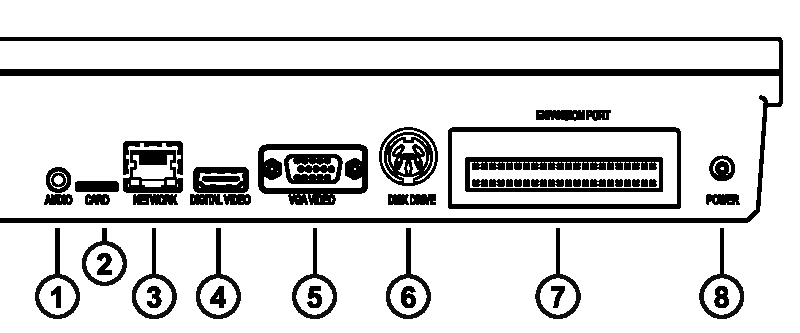
\includegraphics[width=\linewidth]{images/illustrations/mega65-rear.pdf}
\begin{center}
\setlength{\def\arraystretch{1.5}\tabcolsep}{6pt}
\begin{longtable}{ c | l}
	1	& 	3.5 mm-audiojack \\	2	& 	Externe microSD-kaartsleuf\\	3	& 	Netwerk-LAN-poort \\	4	& 	Digitale video-aansluiting (inclusief geluid) \\	5	& 	VGA-videoaansluiting \\	6	& 	Seriële IEC-bus-aansluiting voor schijfstations en printers \\	7	& 	Cartridge-uitbreidingspoort \\	8	& 	Voedingsaansluiting \\
\end{longtable}
\end{center}

\vspace{-1cm}

\section{Aansluitingen aan de zijkant}

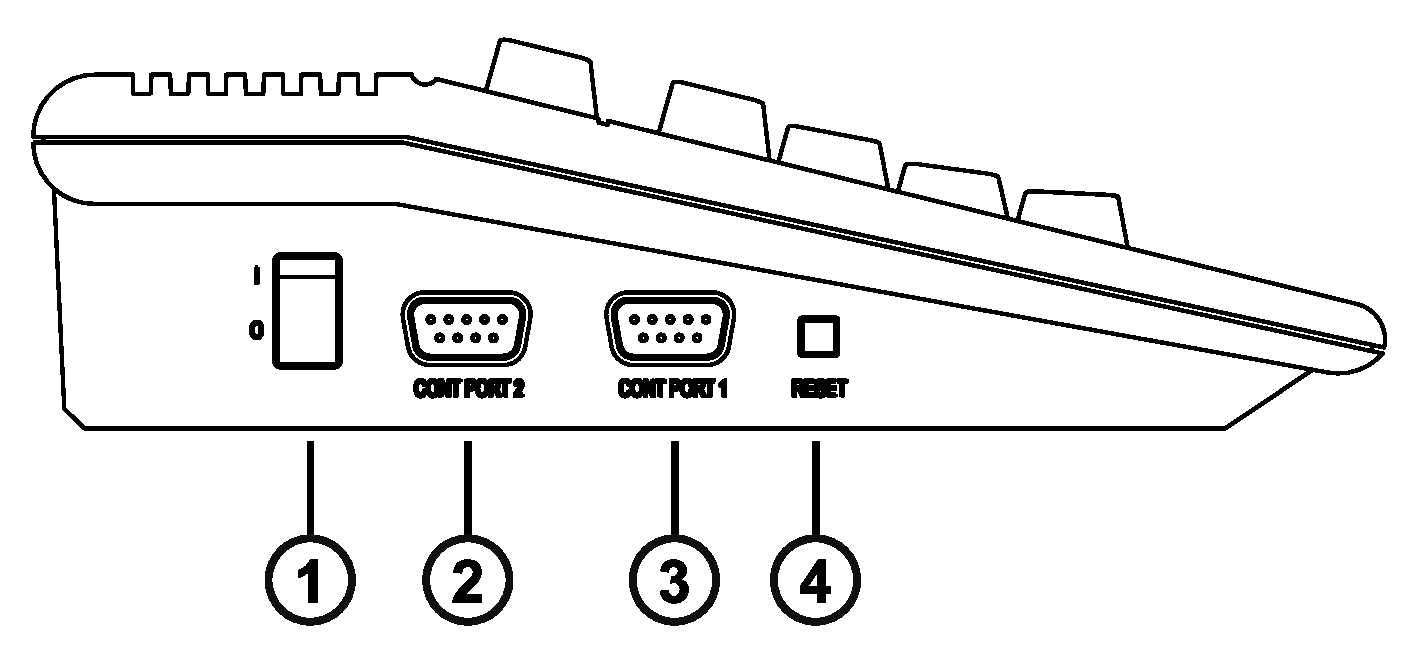
\includegraphics[width=\linewidth]{images/illustrations/mega65-side.pdf}

\begin{center}
\setlength{\def\arraystretch{1.5}\tabcolsep}{6pt}
\begin{longtable}{ c | l}
	1	& 	Aan/uit-schakelaar \\	2	& 	Controllerpoort 2 \\	3	& 	Controllerpoort 1 \\	4	& 	Resetknop \\
\end{longtable}
\end{center}

Op controllerpoorten 1 en 2 kunt u diverse randapparatuur aansluiten, zoals joysticks, peddels of muizen.

\newpage

\section{Beeldscherm en randapparatuur}

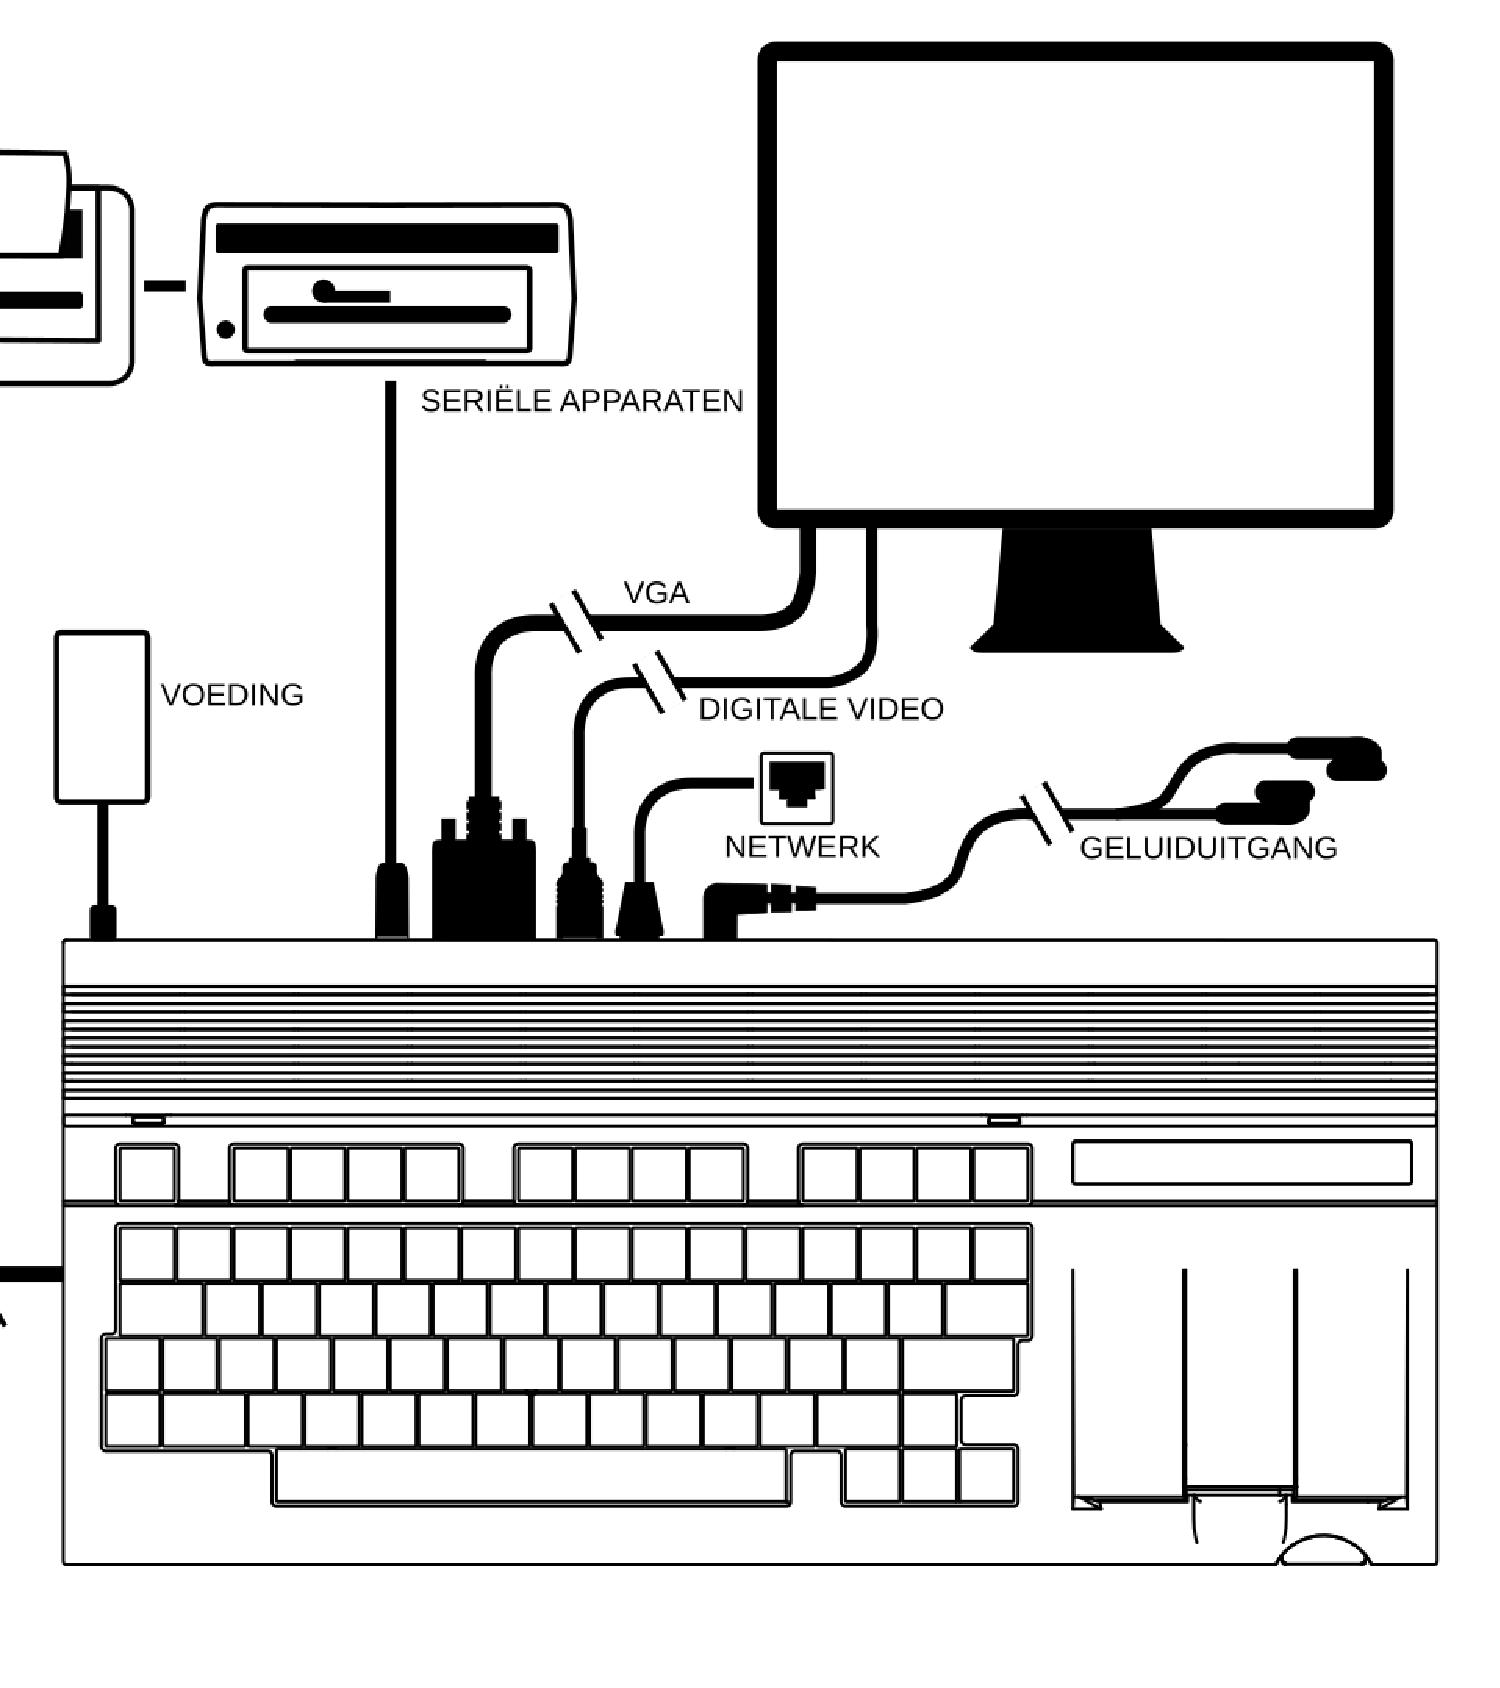
\includegraphics[width=\linewidth]{dutch/images/illustrations/mega65-top.pdf}

U sluit uw MEGA65 als volgt op een beeldscherm aan:
\index{Scherm!Aansluiten}

\begin{enumerate}
	\item Sluit de voeding aan op de voedingsaansluiting van de MEGA65.	\item Als u een VGA-monitor en een VGA-kabel hebt, sluit u het ene uiteinde aan op de VGA-poort van de MEGA65 en het andere uiteinde op uw VGA-monitor.	\item Als u een tv of monitor met een compatibele Digital Video-aansluiting hebt,\footnote{Het type Digital Video-aansluiting heeft een herkenbare commerciële naam van vier letters, doch het MEGA65-project heeft geen licentiekosten betaald om naar dit type met deze naam te verwijzen. Deze {\em Gebruikershandleiding} verwijst hiernaar als de ``Digital Video''-aansluiting.}\index{Digitale video} sluit u het ene uiteinde van uw kabel aan op de Digital Video-poort van de MEGA65 en het andere uiteinde op de Digital Video-poort van uw monitor. Als u een monitor met een DVI-aansluiting hebt, kunt u een Digital Video-naar-DVI-adapter gebruiken.
\end{enumerate}

\newpage
\section{Optionele aansluitingen}
\index{Schijfstations!Aansluiten}
\index{Aansluitingen!IEC}
\index{SD-kaarten!Locaties}
\begin{enumerate}
	\item De MEGA65 bevat een ingebouwd 3.5 inch-diskettestation. U kunt ook oudere Commodore{\textregistered}-diskettestations via de seriële IEC-bus aansluiten, zoals de Commodore 1541, 1571 of 1581. Sluit om deze stations te gebruiken het ene uiteinde van een IEC-kabel aan op het Commodore-diskettestation en het andere uiteinde op de schijfstationsaansluiting van de MEGA65. U kunt ook een SD2IEC-apparaat\index{SD2IEC-apparaat} of een Pi1541-apparaat aansluiten.\index{Pi1541-apparaat} Bij de meeste apparaten kunt u extra diskettestations of met Commodore compatibele printers aan elkaar koppelen.	\item U kunt uw MEGA65 met een standaard ethernetkabel aansluiten op een ethernetnetwerk.	\item Om naar audio van uw MEGA65 te luisteren, kunt u een 3.5 mm-audiojackkabel aansluiten op een audioversterker of een luidsprekersysteem. Als uw systeem over RCA-aansluitingen beschikt, hebt u een 3.5 mm-audiojack-naar-twin-RCA-adapterkabel nodig. De MEGA65 heeft tevens een ingebouwde versterker, zodat u een hoofdtelefoon kunt gebruiken.	\item U kunt een microSD-kaart, type SDHC tussen 4GB en 32GB, in de externe microSD-kaartsleuf aan de achterzijde van de MEGA65 steken. Zie voor meer informatie over het gebruik van de microSD-kaartsleuf ``Kennismaken met SD-kaarten'' op bladzijde \pageref{sec:introducing-sd-cards}.	\item Aan de onderzijde van de MEGA65 geeft een klein klepje toegang tot de interne SD-kaart en twee aansluitingen voor toekomstige hardware-uitbreidingen.
\end{enumerate}

\index{Real-time klok!Batterij plaatsen}
\subsection{De batterij van de real-time klok installeren}

De MEGA65 bevat een real-time klok, welke wordt gebruikt om de tijd en datum op het opstartscherm weer te geven, om tijdstempels toe te voegen aan bestanden die de MEGA65 op uw SD-kaarten schrijft en om de {\bf DT\$}\index{BASIC 65-variabelen!DT} en {\bf TI\$}\index{BASIC 65-variabelen!TI\$}-BASIC-variabelen voor gebruik in programma's te verschaffen. Deze klok gebruikt een CR2032-knoopcelbatterij om de tijd bij te houden wanneer de MEGA65 gedurende langere perioden van de voeding is losgekoppeld. De MEGA65 wordt niet met een batterij geleverd, om problemen met het internationaal verzenden van batterijen te vermijden.\footnote{Vroege modellen van de MEGA65 met de ``R3A''-printplaatrevisie (gemaakt in het jaar 2022) gebruiken een batterij van het type CR1220 voor de real-time klok en de batterij is vereist om de RTC te laten functioneren. Revisie ``R6'' (gemaakt in 2024) gebruikt een batterij van het type CR2032 en de batterij is optioneel voor normaal gebruik.}

{\bf De RTC-batterij is optioneel.} De MEGA65 kan de RTC zonder batterij draaiende houden, zelfs wanneer de computer gedurende meerdere dagen achter elkaar van de voeding is losgekoppeld. Met een batterij kan de computer de tijd gedurende veel langere perioden onthouden. U kunt de klok later altijd opnieuw instellen.

Schakel de computer uit om de batterij te installeren. Gebruik een kruiskopschroevendraaier om de behuizing te openen, waardoor het moederbord zichtbaar wordt.\index{Behuizing!Opening} De behuizing wordt bijeengehouden door drie schroeven, allemaal langs de onderkant van de voorzijde van de behuizing. Til, nadat de schroeven zijn verwijderd, voorzichtig de bovenste helft van de behuizing op. Let op de oriëntatie van de toetsenbordaansluiting en koppel deze vervolgens los.

De batterij bevindt zich tussen de controllerpoorten en de toetsenbordaansluiting.

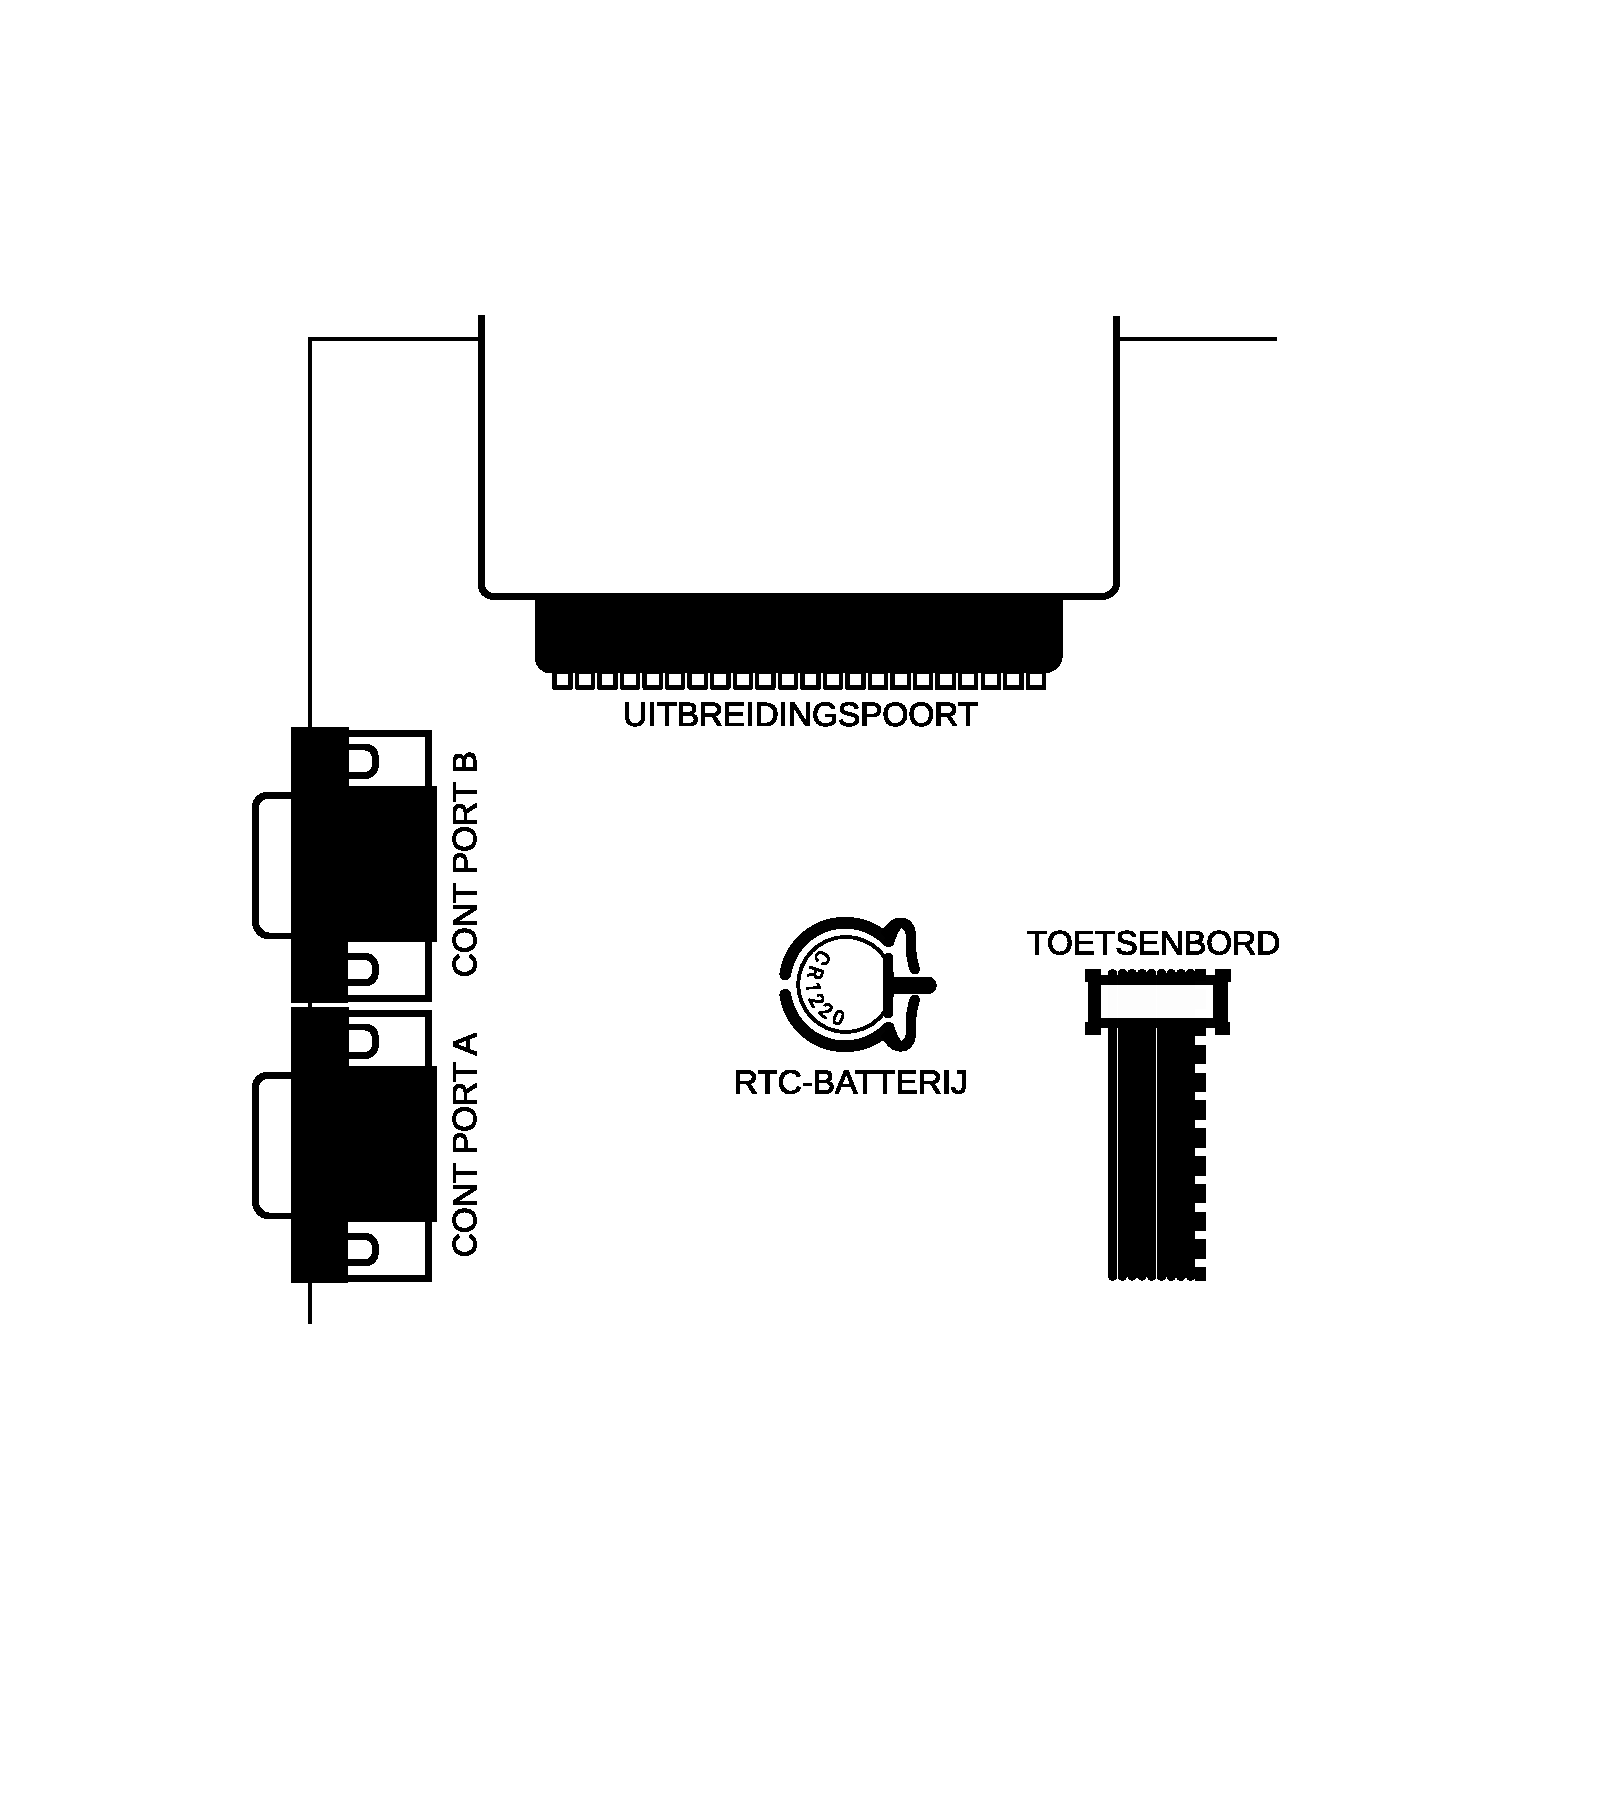
\includegraphics[width=\linewidth]{dutch/images/illustrations/rtc-battery-location.pdf}

Indien u een bestaande batterij verwijdert, duwt u de ontgrendelingshendel van de batterij aan de onderkant (de platte zijde) van de batterijhouder weg van de batterij om deze te verwijderen. Plaats de nieuwe batterij met de positieve zijde (gemarkeerd met {\bf +}) naar boven gericht en druk hem op zijn plaats.

Zodra u uw MEGA65 weer in elkaar hebt gezet, kunt u in het configuratiehulpprogramma de tijd instellen. Zie voor meer informatie over het instellen van de real-time klok het onderdeel over het configuratiehulpprogramma op bladzijde \pageref{sec:configuration-utility}.


\newpage

\section{De MEGA65 inschakelen}
\label{onboarding}

Schakel de MEGA65 in met de aan/uit-schakelaar aan de linkerkant van de computer.

Wanneer u uw MEGA65 voor het eerst inschakelt, toont de computer het scherm voor de initiële configuratie (``on-boarding'').\index{Configuratie!Introductie} Op dit scherm kunt u de tijd en de datum op de real-time klok instellen, de videomodus wijzigen en het geluid testen. Al deze instellingen kunt u later nog wijzigen.

\begin{center}
  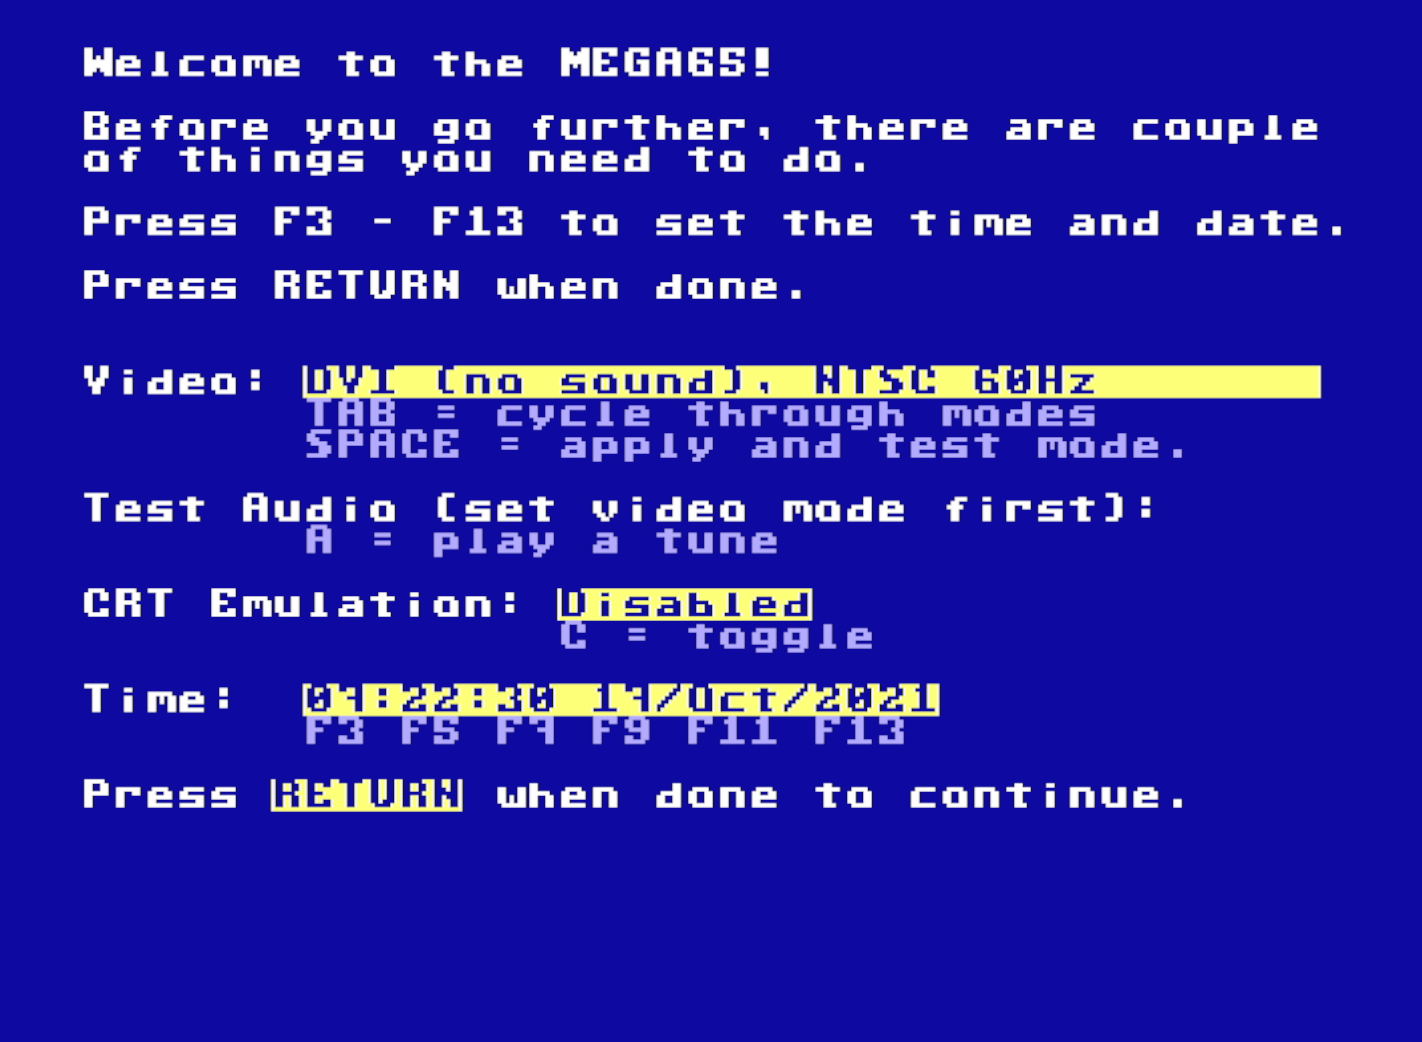
\includegraphics[width=0.7\linewidth]{images/img011_final_boot_01.png}
\end{center}

Voor videomodi kunt u kiezen tussen PAL-emulatie\index{PAL-schermmodus} en NTSC-emulatie\index{NTSC-schermmodus}. Daarnaast kunt u aangeven of uw Digital Video-beeldscherm geluid ondersteunt. Indien u de VGA-videouitgang gebruikt, heeft de Digital Video-geluidsmodus geen effect.

\underline{OPMERKING}: Een DVI-beeldscherm dat geen geluid ondersteunt, werkt niet met de ``enhanced''-geluidsmodus. Bij een dergelijk beeldscherm moet u een videomodus met ``no sound'' selecteren en een luidspreker op de 3.5 mm-audioaansluiting aansluiten.

PAL en NTSC zijn analoge videosignaalformaten die de resolutie en de verticale synchronisatiesnelheid van de videouitgang beïnvloeden, ook wanneer u een modern digitaal beeldscherm gebruikt. Uw beeldscherm ondersteunt mogelijk beide modi of slechts één van beide. U kunt dit scherm gebruiken om de modi met uw beeldscherm te testen.

Selecteer en test uw videoconfiguratie. Druk bijvoorbeeld op \specialkey{TAB} om naar de modus {\bf PAL 50Hz} over te schakelen.
\index{Scherm!PAL/NTSC instellen}
\begin{center}
  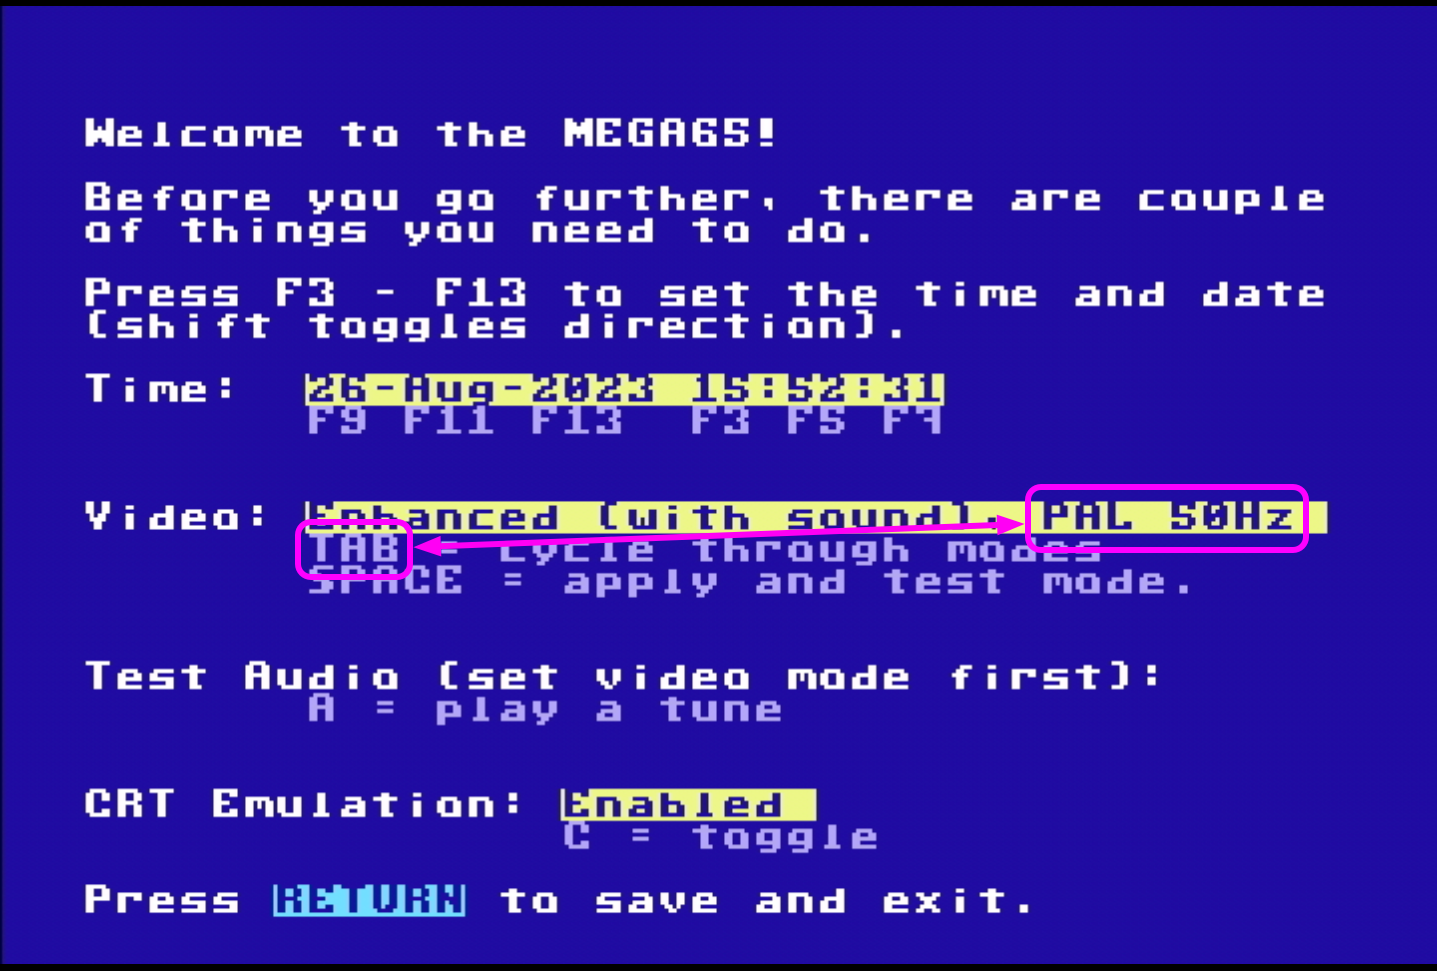
\includegraphics[width=0.7\linewidth]{images/img011_final_boot_02.png}
\end{center}

Druk op \megakey{SPACE} en vervolgens op \megakey{Y} om de nieuwe videomodus te testen.

\begin{center}
  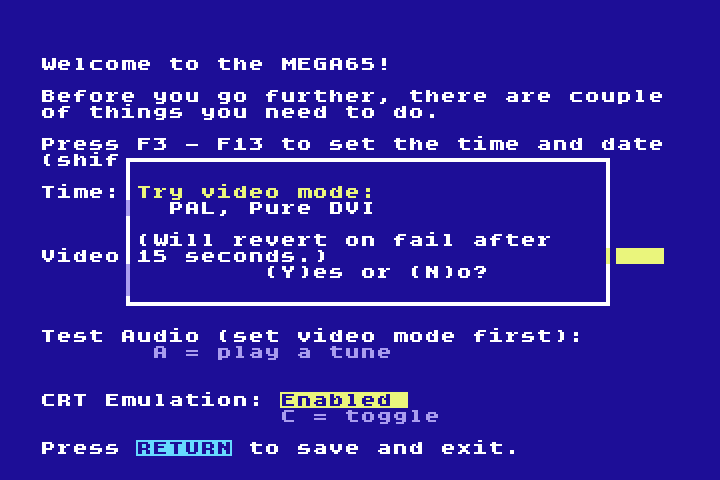
\includegraphics[width=0.7\linewidth]{images/img011_final_boot_03.png}
\end{center}

Druk op \megakey{K} om de nieuwe videomodus te behouden.

\begin{center}
  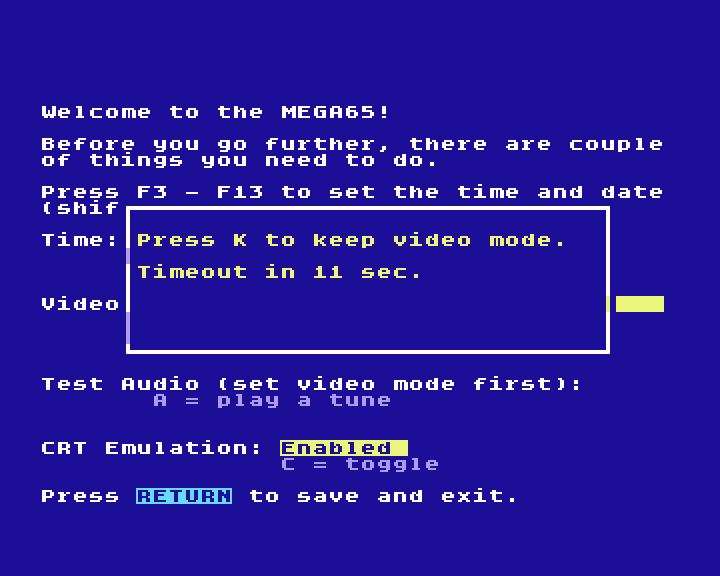
\includegraphics[width=0.7\linewidth]{images/img011_final_boot_04.png}
\end{center}

Maak van deze gelegenheid gebruik om uw geluidsopstelling te testen. Druk op \megakey{A} om een geluid af te spelen.

De optie ``CRT Emulation'' is een leuke keuze bij gebruik van een modern plat scherm. Deze optie voegt verticale tussenruimten toe tussen de pixels om de rasterlijnen van een beeldbuis na te bootsen. Probeer het om te zien of het u bevalt: druk op de toets \megakey{C} om de optie in en uit te schakelen.

Druk ten slotte op \specialkey{RETURN} om de configuratie af te ronden.

Zie voor meer informatie over het configureren van uw MEGA65 hoofdstuk \vref{cha:configuringyourmega}.

\section{De Intro Disk}
\index{Intro Disk}

Nadat u de initiële configuratie hebt afgerond, start uw MEGA65 het Intro Disk-menu. De Intro Disk is een verzameling software van de MEGA65-gemeenschap die enkele van de mogelijkheden van de computer demonstreert. Neem de tijd om door de menu's te bladeren en een aantal demo's uit te proberen. Druk na elke demo op de resetknop aan de linkerkant van de computer om terug te keren naar het Intro Disk-menu.

\begin{center}
  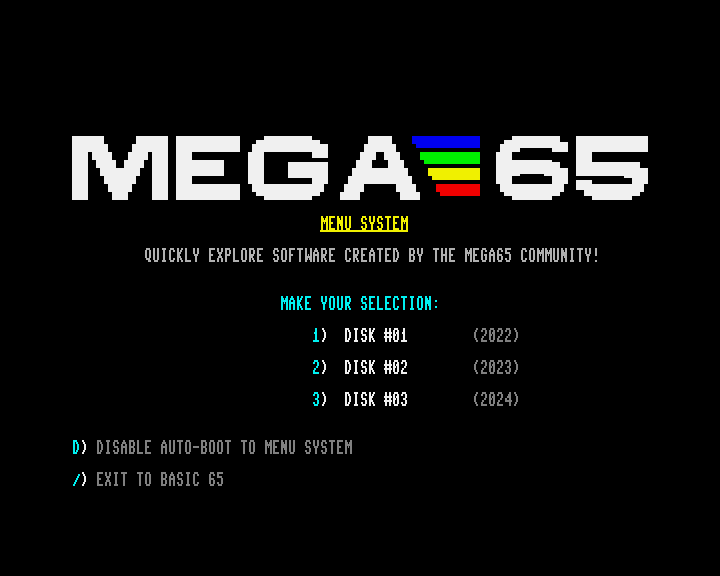
\includegraphics[width=0.7\linewidth]{images/demo_title.png}
\end{center}

Standaard opent het Intro Disk-menu telkens wanneer u de computer inschakelt. Zodra u meer vertrouwd bent met de MEGA65, wilt u dit wellicht uitschakelen. Druk bij het Intro Disk-menu op \megakey{D} om de automatische opstartfunctie van de Intro Disk uit te schakelen.\index{Intro Disk!Uitschakelen}

Druk op \megakey{/} (de schuine streep) om het Intro Disk-menu te verlaten en toegang te krijgen tot BASIC 65. Indien de automatische opstartfunctie van de Intro Disk is uitgeschakeld, gaat de MEGA65 bij het inschakelen rechtstreeks naar BASIC 65.

\begin{center}
  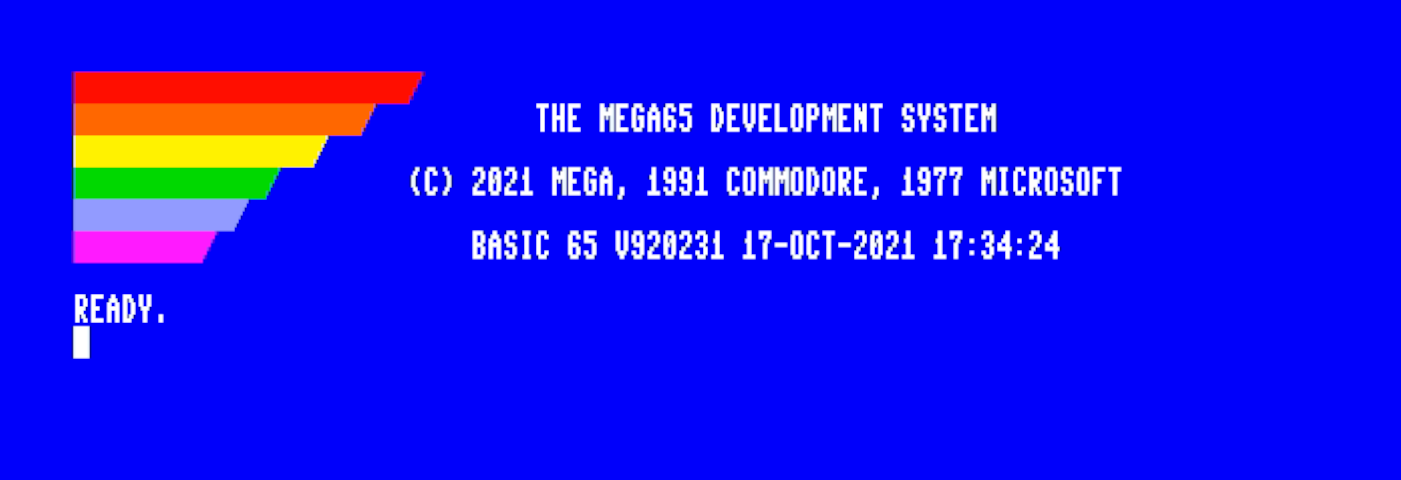
\includegraphics[width=0.7\linewidth]{images/img011_final_boot_06.png}
\end{center}

\section{De cursor}

Het knipperende blokje onder de \screentext{READY}-prompt\index{READY-prompt} wordt de \emph{cursor} genoemd. De cursor geeft aan dat de computer klaar is om invoer te ontvangen. Wanneer u toetsen op het toetsenbord indrukt, verschijnen de bijbehorende tekens op het scherm. De tekens verschijnen op de huidige cursorpositie en de cursor schuift na elke toetsaanslag een positie op.

Hier kunt u commando's typen waarmee u bijvoorbeeld een programma kunt laden. U kunt ook beginnen met het intypen van programmacode!

\chapter{Aan de slag}\addtocontents{toc}{\protect\setcounter{tocdepth}{2}}
\hypersetup{bookmarksdepth=5}

\section{Toetsenbord}
\label{cha:getting-started}
\index{Toetsenbord}

Nu alles is aangesloten, is het tijd om vertrouwd te raken met het toetsenbord van de MEGA65.

Wellicht valt u op dat het toetsenbord enigszins afwijkt van de toetsenborden van andere hedendaagse computers. De meeste toetsen staan op vertrouwde posities, maar er zijn enkele gespecialiseerde toetsen en sommige toetsen hebben speciale grafische symbolen op de voorkant.

In sommige beeldschermmodi zijn de grafische symbolen te typen, net als letters, cijfers en leestekens. De volledige verzameling tekens staat bekend als de {\em PETSCII-tekenset}.\index{PETSCII}

\subsection{Speciale toetsen}

\subsubsection{RETURN}
\index{Toetsenbord!RETURN}
Wanneer u op \specialkey{RETURN} drukt, slaat de computer de informatie die u hebt getypt op in het geheugen. De computer voert vervolgens een opdracht uit, bewaart enkele gegevens of toont een foutmelding indien u een vergissing hebt gemaakt.

\subsubsection{SHIFT}
\index{Toetsenbord!Shifttoetsen}
De twee \specialkey{SHIFT}-toetsen bevinden zich links en rechts. Zij werken vrijwel hetzelfde als de Shift-toets van een gewoon toetsenbord en vervullen daarnaast nog enkele speciale functies.

In de modus met hoofdletters levert het ingedrukt houden van \specialkey{SHIFT} en het indrukken van een toets met twee grafische symbolen op de voorkant het rechter symbool van die toets op. Zo toont \specialkey{SHIFT} samen met \megakey{J} het teken \graphicsymbol{J}.

In de modus met kleine letters geeft het indrukken van \specialkey{SHIFT} en een lettertoets de hoofdletter van die toets weer.

Om de Griekse letter $\pi$ (pi) te typen, houdt u \specialkey{SHIFT} ingedrukt en drukt u op \megakeywhite{$\uparrow$}.

Het ingedrukt houden van \specialkey{SHIFT} en het indrukken van een functietoets roept de functie op die op de voorkant van die toets staat vermeld. Zo activeert \specialkey{SHIFT} samen met \megakey{F1} de functie \megakey{F2}.


\subsubsection{SHIFT LOCK}
\index{Toetsenbord!SHIFT LOCK}
Naast \specialkey{SHIFT} is er de \specialkey{SHIFT\\LOCK}-toets. Druk op deze toets om de Shift-functie vast te zetten. Wanneer \specialkey{SHIFT\\LOCK} verlicht is, toont elke toets die u indrukt het bijbehorende teken op het scherm, alsof u \specialkey{SHIFT} ingedrukt houdt. Dit geldt ook voor speciale grafische tekens.

\subsubsection{CTRL}
\index{Toetsenbord!CTRL}
\specialkey{CTRL} is de Control-toets. Door \specialkey{CTRL} ingedrukt te houden en een andere toets in te drukken, kunt u Controlcodes uitvoeren. Zo kunt u met \specialkey{CTRL} ingedrukt en één van de cijfertoetsen (van \megakey{1} tot \megakey{8}) de tekstkleur wijzigen. De kleur die op de bovenste rij van de voorkant van de cijfertoets is afgedrukt, wordt gebruikt. Het ingedrukt houden van \specialkey{CTRL} en het indrukken van \megakey{9} of \megakey{0} schakelt de modus voor omgekeerde tekst in en uit.

Enkele voorbeelden hiervan vindt u op bladzijde \pageref{sec:screen-editor} en alle Controlcodes staan vermeld op bladzijde \pageref{appendix:controlcodes}.

Wanneer een programma met {\bf LIST} op het scherm wordt weergegeven, vertraagt het ingedrukt houden van \specialkey{CTRL} de weergave van elke regel. Meer over het commando {\bf LIST} leest u op bladzijde \pageref{BASIC 65 Commands!LIST}.\index{BASIC 65-commando's!LIST}

Het ingedrukt houden van \specialkey{CTRL} en het indrukken van \megakey{*} opent de Matrix Mode Debugger (raadpleeg {\bf Het grote Mega65-boek} voor meer details).

\subsubsection{RUN/STOP}
\index{Toetsenbord!RUN STOP}
Normaal gesproken stopt het indrukken van \specialkey{RUN\\STOP} de uitvoering van een programma. Wanneer u \specialkey{SHIFT} ingedrukt houdt en op \specialkey{RUN\\STOP} drukt, voert u met {\bf RUN} het eerste programma van de schijf uit.\index{BASIC 65-commando's!RUN}

Sommige programma's onderscheppen de \specialkey{RUN\\STOP}-toets en kunnen op deze wijze niet worden gestopt.

U kunt uw MEGA65 naar de {\bf Machinetaalmonitor}\index{Machinetaalmonitor} opstarten door \specialkey{RUN\\STOP} ingedrukt te houden en de resetknop aan de linkerkant van de computer in te drukken (of door de toets ingedrukt te houden terwijl u de computer inschakelt).

\subsubsection{RESTORE}
\index{Toetsenbord!RESTORE}
Het computerscherm kan naar een schone toestand worden teruggebracht zonder het geheugen te wissen door \specialkey{RUN\\STOP} ingedrukt te houden en \widekey{RESTORE} in te drukken. Deze combinatie herstelt tevens de vectoren van het besturingssysteem en initialiseert de schermeditor opnieuw, hetgeen dit tot een handige combinatie maakt indien de computer een beetje in de war is geraakt.

Sommige programma's onderscheppen de toetsencombinatie \specialkey{RUN\\STOP} + \widekey{RESTORE} en kunnen op deze wijze niet worden gereset.

U kunt de {\bf Freezer} ook oproepen door \widekey{RESTORE} één seconde ingedrukt te houden en de toets vervolgens los te laten. U kunt meer over de Freezer lezen op bladzijde \pageref{sec:freezer}.\index{Freezer-menu}

\subsubsection{De cursor-toetsen}
\index{Toetsenbord!Cursortoetsen}
\nopagebreak
De cursor-toetsen staan rechtsonder op het toetsenbord. Met deze vier richtingtoetsen kunt u de cursor naar elke gewenste positie verplaatsen voor het bewerken van tekst op het scherm.

De cursor beweegt in de richting die op de toetsen is aangegeven: \megakey{$\leftarrow$} \megakey{$\uparrow$} \megakey{$\rightarrow$} \megakey{$\downarrow$}.

U hoeft een cursor-toets niet telkens opnieuw in te drukken. Indien u de cursor over een grote afstand moet verplaatsen, kunt u de toets ingedrukt houden. Wanneer u klaar bent, laat u de toets gewoon los.

\subsubsection{De pijltjestoetsen}
\index{Toetsenbord!Pijltjestoetsen}
Deze toetsen verschillen van de cursor-toetsen. Het zijn \megakeywhite{$\leftarrow$} (naast \megakey{1}) en \megakeywhite{$\uparrow$} (naast \widekey{RESTORE}). Beide pijltjestoetsen worden gebruikt in diverse BASIC-functies en escape-sequenties.

Zo kan \megakeywhite{$\leftarrow$} als snelkoppeling voor {\bf SAVE}\index{BASIC 65-commando's!SAVE} dienen en wordt \megakeywhite{$\uparrow$} gebruikt om een getal tot een macht te verheffen (hetgeen gelijkstaat aan het getal een opgegeven aantal malen met zichzelf te vermenigvuldigen).

U kunt meer lezen over de beschikbare escape-sequenties op bladzijde \pageref{escape-sequences}.

Deze twee PETSCII-specifieke toetsen worden in de MEGA65-literatuur altijd met een witte achtergrond weergegeven.

Het is ook mogelijk de cursor met \specialkey{SHIFT} en \megakey{$\downarrow$} omhoog en met \specialkey{SHIFT} en \megakey{$\rightarrow$} naar links te verplaatsen. Dit is een erfenis van de Commodore 64, welke slechts twee cursor-toetsen had.

\subsubsection{INSerT/DELete}
\index{Toetsenbord!INST DEL}
De toets \specialkey{INST\\DEL}, de meest rechtse toets van de bovenste rij, is de INSERT/DELETE-toets. Wanneer u \specialkey{INST\\DEL} indrukt, wordt het teken links daarvan verwijderd en worden alle tekens rechts daarvan één positie naar links verschoven.

Om een teken in te voegen, houdt u \specialkey{SHIFT} ingedrukt en drukt u op \specialkey{INST\\DEL}. Het teken onder de cursor en de tekens rechts van de cursor worden naar rechts verschoven. Op de nieuw vrijgekomen plaats kunt u vervolgens een letter, een cijfer of elk ander teken typen.


\subsubsection{CLeaR/HOME}
\index{Toetsenbord!CLR HOME}
De toets \specialkey{CLR\\HOME} is de CLEAR/HOME-toets. Het indrukken van \specialkey{CLR\\HOME} verplaatst de cursor naar de linkerbovenhoek van het scherm.

Door \specialkey{SHIFT} ingedrukt te houden en op \specialkey{CLR\\HOME} te drukken, wist u het volledige scherm {\it en} plaatst u de cursor in de linkerbovenhoek van het scherm.

Indien u per ongeluk \specialkey{CLR\\HOME} indrukt, kunt u de cursor naar zijn vorige positie terugbrengen door \specialkey{ESC} en vervolgens \specialkey{CLR\\HOME} in te drukken.

\subsubsection{De MEGA-toets}
\index{Toetsenbord!MEGA-toets}
De \megasymbolkey of de MEGA-toets biedt een aantal verschillende functies en kan worden gebruikt om speciale hulpprogramma's op te starten.

Door \specialkey{SHIFT} ingedrukt te houden en \megasymbolkey in te drukken, schakelt u tussen de kleine- en de hoofdlettermodus.

Door \megasymbolkey ingedrukt te houden en een willekeurige toets met twee grafische symbolen op de voorkant in te drukken, geeft de computer het meest linkse grafische symbool op het scherm weer. Zo geven \megasymbolkey en \megakey{D} het symbool \graphicsymbol{d} weer.

Door \megasymbolkey ingedrukt te houden en een cijfertoets in te drukken, schakelt u over naar een secundaire kleur, d.w.z. de kleur die op de onderste rij aan de voorkant van de cijfertoets is afgedrukt.

Door \megasymbolkey ingedrukt te houden en \specialkey{TAB} in te drukken, opent u de Matrix Mode Debugger (zie voor meer details {\bf Het grote Mega65-boek}).

Indien u de MEGA65 inschakelt, of de resetknop aan de linkerkant indrukt terwijl u \megasymbolkey ingedrukt houdt, schakelt de MEGA65 over naar de GO64-modus.\index{Commodore 64!GO64-modus}

\subsubsection{NO SCROLL}
\index{Toetsenbord!NO SCROLL}
Indien een programma met {\bf LIST} naar het scherm wordt afgedrukt, onderbreekt u de schermuitvoer door \specialkey{NO\\SCROLL} in te drukken. Druk een willekeurige toets in om de pauze op te heffen.

Deze functie is niet beschikbaar in de GO64-modus.\index{Commodore 64!GO64-modus}

\subsubsection{De functietoetsen}
\index{Toetsenbord!Functietoetsen}
Er zijn zeven functietoetsen beschikbaar die door softwaretoepassingen gebruikt kunnen worden. \megakey{F1} \megakey{F3} \megakey{F5} \megakey{F7} \megakey{F9} \megakey{F11} en \megakey{F13} kunnen worden gebruikt om speciale functies uit te voeren.

Houd \specialkey{SHIFT} ingedrukt om \megakey{F2} tot en met \megakey{F14} te gebruiken, zoals op de voorkant van elke functietoets is aangegeven.
\index{Toetsenbord!Shifttoetsen}
In de GO64-modus zijn alleen de functietoetsen \megakey{F1} tot en met \megakey{F8} beschikbaar.\index{Commodore 64!GO64-modus}

\subsubsection{HELP}
\index{Toetsenbord!HELP}
\specialkey{HELP} kan door software worden gebruikt en fungeert tevens als \megakey{F15}.

\subsubsection{ALT}
\index{Toetsenbord!ALT}
Software kan specifieke functies uitvoeren door \specialkey{ALT} ingedrukt te houden en tegelijkertijd andere toetsen in te drukken. Deze functie is niet beschikbaar in de GO64-modus.\index{Commodore 64!GO64-modus}

Door \specialkey{ALT} ingedrukt te houden terwijl u de MEGA65 inschakelt, opent u het hulpprogrammamenu.\index{Hulpprogrammamenu} U kunt een SD-kaart formatteren, het MEGA65-configuratiehulpprogramma\index{Configuratie!Hulpprogramma} openen om de standaard videomodus te kiezen en andere instellingen te wijzigen, of uw toetsenbord testen.

\subsubsection{CAPS LOCK}
\index{Toetsenbord!CAPS LOCK}
\specialkey{CAPS\\LOCK} werkt op dezelfde wijze als \specialkey{SHIFT\\LOCK} in de C65- en MEGA65-modus, maar heeft alleen invloed op de lettertoetsen.

Indien de MEGA65 is ingesteld om op een lagere processorsnelheid te draaien, zoals in de GO64-modus,\index{Commodore 64!GO64-modus} kunt u \specialkey{CAPS\\LOCK} ingedrukt houden om de processor tijdelijk op volledige snelheid te laten draaien. Dit is in de GO64-modus nuttig om bijvoorbeeld het laden vanaf het interne schijfstation of de SD-kaart te versnellen, of om het uitpakproces na het uitvoeren van een programma aanzienlijk te versnellen. De MEGA65-modus draait standaard op maximale snelheid.

\addtocontents{toc}{\protect\setcounter{tocdepth}{5}}


\section{De schermeditor}
\label{sec:screen-editor}

Wanneer u uw MEGA65 inschakelt of reset, verschijnt het volgende scherm:\footnote{Hiervoor moet u het Intro Disk-menu hebben uitgeschakeld. Indien het Intro Disk-menu draait, drukt u op ``/'' (schuine streep) om naar dit scherm terug te keren.}

\begin{center}
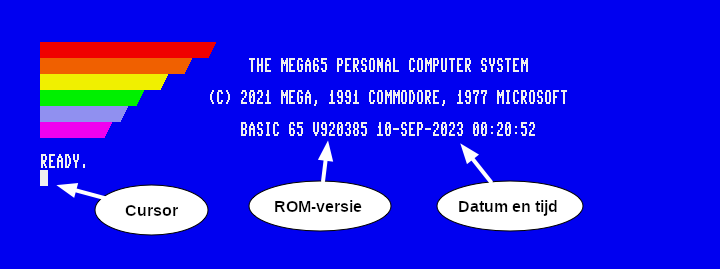
\includegraphics[width=0.9\linewidth]{dutch/images/introduction-screen/layout.png}
\end{center}

De kleurbalken linksboven in het scherm kunt u gebruiken als richtlijn om de kleuren van uw beeldscherm te kalibreren. Het scherm toont tevens de naam van het systeem, de copyrightmelding en de ROM-versie. De weergegeven datum en tijd zijn afkomstig van de interne RTC (Real-Time Clock) op het moment dat de computer werd ingeschakeld. U kunt de datum en tijd instellen in het configuratiehulpprogramma.

Ten slotte ziet u de \screentext{READY}-prompt en de knipperende cursor.

U kunt beginnen met typen op het toetsenbord en de tekens verschijnen op de cursorpositie. Na elke toetsaanslag schuift de cursor één positie verder.

U kunt ook omgekeerde tekst of kleurbalken maken door \specialkey{CTRL} ingedrukt te houden en \megakey{9} of \megakey{R} in te drukken. Hiermee schakelt u de modus voor omgekeerde tekst in. Indien deze modus is ingeschakeld, kunt u de spatiebalk \megakey{Space} indrukken en ingedrukt houden. Terwijl u dat doet, wordt een witte balk over het scherm getekend.
\index{Toetsenbord!CTRL}
U kunt de huidige kleur wijzigen door \specialkey{CTRL} ingedrukt te houden en een cijfertoets in te drukken (van \megakey{1} tot \megakey{8}). Indien u bijvoorbeeld \specialkey{CTRL} ingedrukt houdt en \megakey{1} indrukt, verandert de kleur in zwart. Wanneer u nu de spatiebalk \megakey{Space} ingedrukt houdt, wordt een zwarte balk getekend. Indien u de kleur blijft wijzigen en de spatiebalk \megakey{Space} indrukt, krijgt u een effect dat vergelijkbaar is met de volgende afbeelding:

\begin{center}
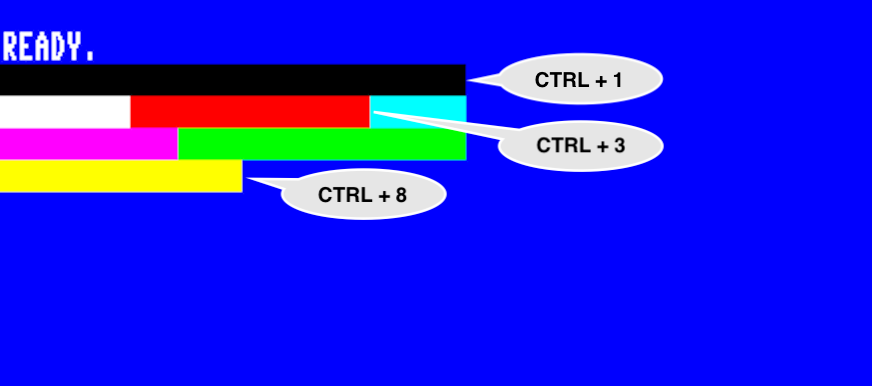
\includegraphics[width=0.7\linewidth]{images/introduction-screen/colour-bars.png}
\end{center}

U kunt de modus voor omgekeerde tekst uitschakelen door \specialkey{CTRL} ingedrukt te houden en \megakey{0} in te drukken.

Nog acht kleuren kunt u selecteren door \megasymbolkey ingedrukt te houden en een toets van \megakey{1} tot \megakey{8} in te drukken.\index{Toetsenbord!MEGA-toets}

De kleur die op de onderste rij aan de voorkant van de cijfertoets is afgedrukt, wordt gebruikt. Indien u bijvoorbeeld \megasymbolkey ingedrukt houdt terwijl u \megakey{4} indrukt, wordt donkergrijs gebruikt. Voor toegang tot nog 16 kleuren van het alternatieve/rainbow-palet verwijzen wij u naar de sneltoets \specialkey{CTRL} + \megakey{A}, die beschreven staat op bladzijde \pageref{appendix:controlcodes}.

\underline{OPMERKING}:
\begin{itemize}
  \item {\bf Zinnebeeldmodus}: Indien u \megakey{"} indrukt om een tekenreeks te beginnen en vervolgens probeert kleuren te wijzigen, tekst om te keren, de cursor te verplaatsen of de toets \specialkey{CLR\\HOME} te gebruiken, verschijnen er in plaats van dat deze acties onmiddellijk plaatsvinden, grappige PETSCII\index{PETSCII}-tekens. Dit komt door een voorziening van BASIC die {\it zinnebeeldmodus} heet en waarmee u dergelijke acties in een tekenreeks kunt coderen, zodat u ze op een later tijdstip kunt uitvoeren (bijvoorbeeld via een {\bf PRINT}-instructie in uw programma's). Om de zinnebeeldmodus te beëindigen typt u eenvoudig een nieuwe \megakey{"} om het einde van uw tekenreeks aan te geven.  \item {\bf Invoegmodus}: Een vergelijkbare voorziening is de {\it invoegmodus}. Het aantal keren dat u \specialkey{SHIFT} + \specialkey{INST\\DEL} indrukt om enkele spaties in te voegen, is gelijk aan het aantal toetsaanslagen dat erop volgt en dat zich volgens dezelfde beginselen als de zinnebeeldmodus gedraagt.  \item U kunt beide modi ook geforceerd beëindigen door \specialkey{ESC} en daarna \megakey{O} in te drukken.
\end{itemize}

\needspace{4cm}
U kunt eenvoudig leuke afbeeldingen maken door deze kleuren en letters te gebruiken. Hieronder ziet u een voorbeeld van wat een vierdejaarsstudent tekende:

\begin{center}
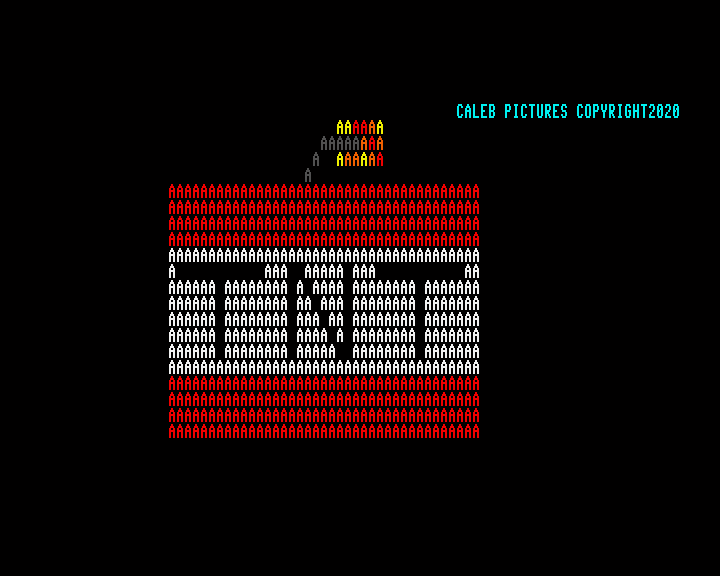
\includegraphics[width=0.7\linewidth]{images/caleb-PETSCII-TNT-final}
\end{center}

Wat gaat u tekenen?

\needspace{2cm}
\textbf{Functies}

Functies die gebruikmaken van \specialkey{CTRL} worden \textbf{Controlcodes} genoemd. Functies die gebruikmaken van \megasymbolkey worden \textbf{Megacodes} genoemd. Er bestaan ook functies die via \specialkey{SHIFT} worden aangeroepen; deze worden \textbf{Shiftcodes} genoemd.

Ten slotte maakt \specialkey{ESC} het gebruik van \textbf{escape-sequenties} mogelijk.

Over al deze functies leest u meer op bladzijde \pageref{appendix:controlcodes}.

\needspace{2cm}
\textbf{Escape-sequenties}

\index{Toetsenbord!Escape-reeksen}
Escape-sequenties worden iets anders uitgevoerd dan een controlcode of een shiftcode. In plaats van de modificatietoets ingedrukt te houden, voert u een escape-sequentie uit door \specialkey{ESC} in te drukken, deze los te laten en vervolgens de gewenste toets in te drukken.

Om bijvoorbeeld te schakelen tussen de 80-kolomsmodus en de 40-kolomsmodus drukt u \specialkey{ESC} in, laat u deze los en drukt u vervolgens op \megakey{X}.

Er zijn nog meer tekstmodi beschikbaar. U kunt knipperende tekst maken door \specialkey{CTRL} ingedrukt te houden en op \megakey{O} te drukken. Alle tekens die u intypt, zullen knipperen. Schakel de knippermodus uit door \specialkey{ESC} en daarna \megakey{O} in te drukken.


\section{Functionaliteit van de editor}

De schermeditor van de MEGA65\index{Schermeditor} biedt verschillende manieren om de cursor snel over het scherm te verplaatsen, zodat u productiever kunt werken.

Druk bijvoorbeeld op \specialkey{CLR\\HOME} om naar de startpositie op het scherm te gaan. Houd \specialkey{CTRL} ingedrukt en druk enkele malen op \megakey{W}. Dit is de functie \textbf{Word Advance}, die uw cursor naar het volgende woord of afdrukbare teken verplaatst.

U kunt naar eigen inzicht tabposities op het scherm instellen. Druk op \specialkey{CLR\\HOME} en vervolgens op \megakey{$\rightarrow$} om de cursor naar de vierde kolom te verplaatsen. Houd \specialkey{CTRL} ingedrukt en druk op \megakey{X} om een tab in te stellen. Verplaats de cursor nog 16 posities naar rechts en druk opnieuw op \specialkey{CTRL} en \megakey{X} om een tweede tab in te stellen.

Druk op \specialkey{CLR\\HOME} om terug te keren naar de startpositie. Houd \specialkey{CTRL} ingedrukt en druk op \megakey{I}. Dit is de functie \textbf{Forward Tab}. Uw cursor springt naar de vierde positie. Druk opnieuw op \specialkey{CTRL} en \megakey{I}. Uw cursor verplaatst zich naar positie 8. Standaard is elke achtste positie reeds als tabpositie ingesteld. De vierde en de twintigste positie zijn derhalve toegevoegd aan de bestaande tabposities. U kunt op \specialkey{CTRL} en \megakey{I} blijven drukken om door te springen naar de zestiende en twintigste positie.

\subsection{Een venster maken}
\index{Toetsenbord!Escape-reeksen}
\index{Vensters!Escape-reeksen}

U kunt een venster instellen op het werkscherm van de MEGA65. Verplaats uw cursor naar het begin van de tekst ``BASIC 65''. Druk op \specialkey{ESC} en daarna op \megakey{T}. Verplaats de cursor 10 regels omlaag en 15 posities naar rechts.

Druk op \specialkey{ESC} en daarna op \megakey{B}. Alles wat u typt, blijft binnen dit venster.

Indien u bijvoorbeeld \screentext{LIST} typt om een programma weer te geven, blijft de listing beperkt tot het venstergedeelte dat u hebt aangegeven:

\begin{center}
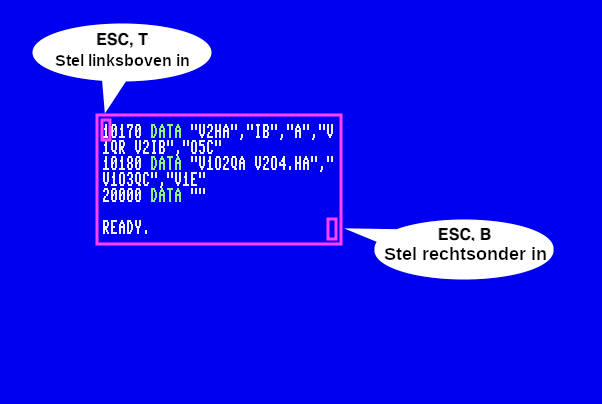
\includegraphics[width=0.7\linewidth]{dutch/images/set-window.png}
\end{center}

Druk tweemaal op \specialkey{CLR\\HOME} om het venster te verlaten en terug te keren naar het volledige scherm.

\subsection{Aanvullende ASCII-tekens}

U hebt misschien opgemerkt dat zich op het toetsenbord van de MEGA65 een aantal ASCII-tekens bevindt die van oudsher geen deel uitmaken van de PETSCII-tekenset\index{PETSCII}. Om deze tekens te gebruiken:

\begin{itemize}
  \item Typ \screentext{FONT A} of \screentext{FONT B}.  \item Druk op \megasymbolkey + \specialkey{SHIFT} om over te schakelen naar kleine letters.
\end{itemize}

U kunt die extra ASCII-tekens nu typen door \megasymbolkey ingedrukt te houden en de toets in te drukken.

\begin{center}
  \begin{tabular}{|l|c|l|}
  \hline
  \textbf{Naam} & \textbf{Teken} & \textbf{Toetscombinatie} \\
  \hline
  Backtick & \texttt{\`} & \megasymbolkey + \megakeywhite{$\leftarrow$} \\
  \hline
  Tilde & \texttt{\~} & \megasymbolkey + \megakey{,} (komma) \\
  \hline
  Verticale streep & \texttt{|} & \megasymbolkey + \megakey{.} (punt) \\
  \hline
  Backslash & \texttt{\textbackslash} & \megasymbolkey + \megakey{/} \\
  \hline
  Linker accolade & \texttt{\{} & \megasymbolkey + \megakey{:} \\
  \hline
  Rechter accolade & \texttt{\}} & \megasymbolkey + \megakey{;} \\
  \hline
  Underscore & \texttt{\_} & \megasymbolkey + \megakey{=} \\
  \hline
  \end{tabular}
\end{center}

De alternatieve lettertypen vervangen tekens uit de oorspronkelijke PETSCII-tekenset door deze symbolen. Om terug te keren naar de PETSCII-tekenset, typt u \screentext{FONT C}.

\subsection{Hoofdletters en kleine letters}

\megasymbolkey + \specialkey{SHIFT} schakelt voor het volledige scherm tussen tekst in hoofdletters en tekst in kleine letters. Dit werkt ook tijdens de uitvoering van een programma, zodat u het kunt aanpassen wanneer een programma zich in de verkeerde modus bevindt.


\section{Het Freezer-menu}
\label{sec:freezer}
\index{Freezer-menu}
\nopagebreak
De MEGA65 brengt het grootste deel van zijn tijd door als een Commodore 65-computer, door een programma uit te voeren of te wachten op instructies in de BASIC-omgeving. Uw MEGA65 beschikt over extra voorzieningen die geen deel uitmaakten van het oorspronkelijke C65-ontwerp. U hebt toegang tot veel van deze voorzieningen via het Freezer-menu.

Om het Freezer-menu te openen, houdt u de toets \widekey{RESTORE} één seconde ingedrukt en laat u deze vervolgens los. De MEGA65 onderbreekt zijn bezigheden, laat de randkleur flikkeren en opent vervolgens het Freezer-menu. Het programma dat op dat moment liep, blijft in het geheugen staan en kan worden hervat door op de toets \megakey{F3} te drukken. U kunt het draaiende programma ook afbreken en de MEGA65 resetten door op \megakey{F5} te drukken.

\begin{center}
  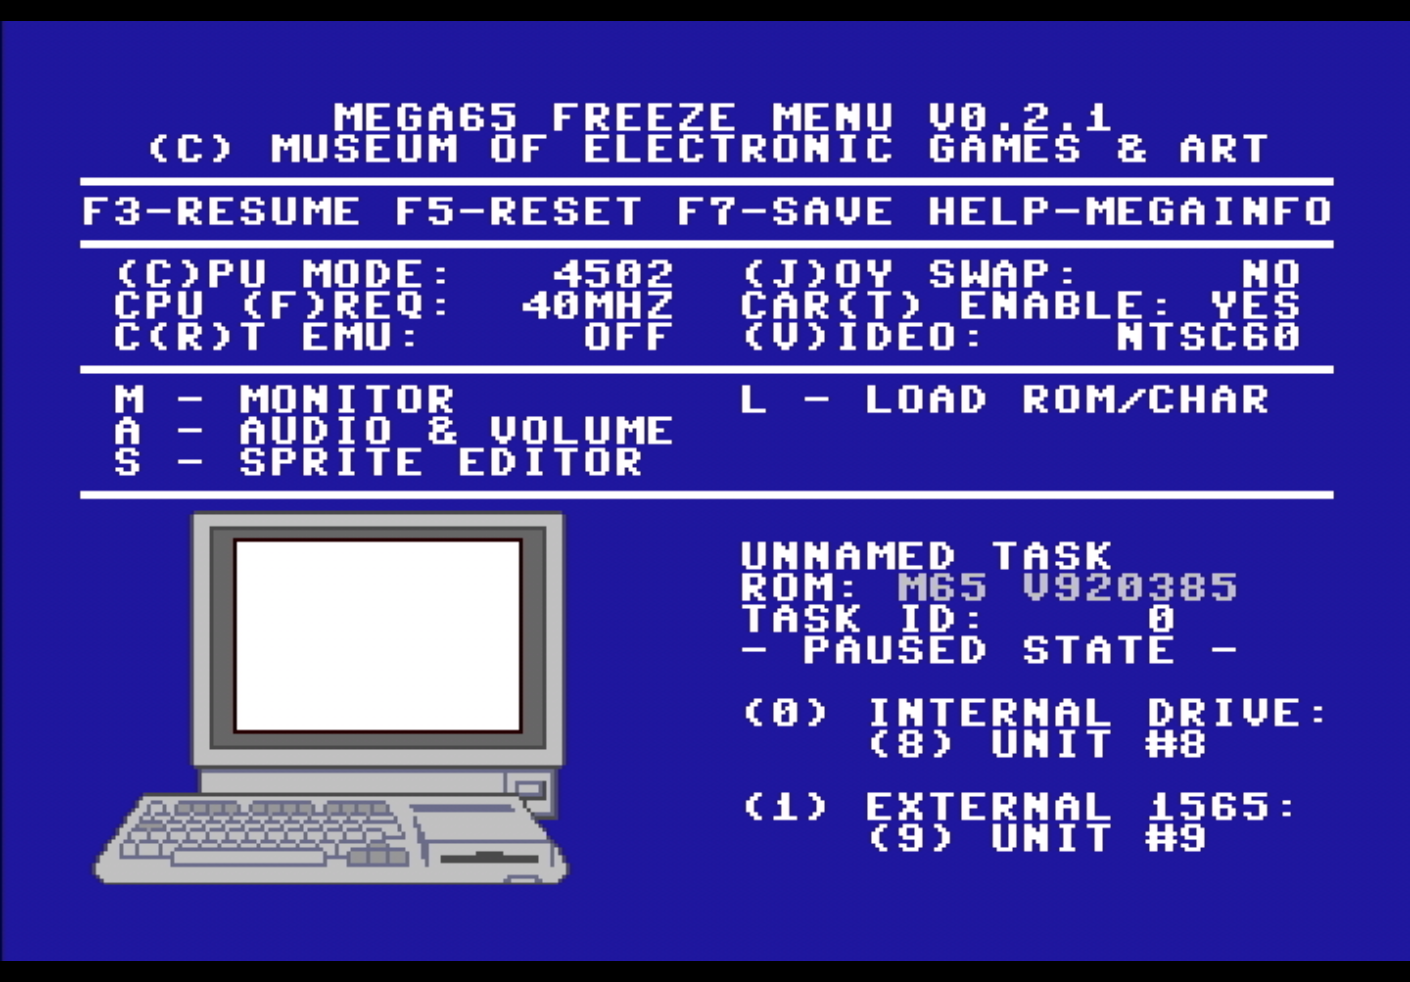
\includegraphics[width=0.7\linewidth]{images/freezer.png}
\end{center}

Een functie om te onthouden tijdens het spelen van spellen is ``(J)OY SWAP''. Deze functie laat de joystickpoorten van nummer wisselen. Hebt u een joystick in poort 2 en start u een spel dat een joystick in poort 1 verwacht, dan hoeft u de joystick niet los te koppelen en opnieuw aan te sluiten. Open in plaats daarvan het Freezer-menu, druk op \megakey{J} om de poortnummers om te wisselen en hervat vervolgens uw spel.

Het menu wordt ``Freezer'' genoemd omdat de toestand van de MEGA65 bevroren blijft terwijl u het menu gebruikt. Het Freezer-menu kan meerdere freeze-toestanden opslaan en u kunt tussen deze toestanden schakelen. Om de huidige toestand op te slaan, gaat u met de rechtercursortoets naar een ongebruikt {\it freeze-slot} en drukt u vervolgens op \megakey{F7}. Wanneer de rand ophoudt met knipperen, is de toestand opgeslagen. Om een toestand te herstellen, gaat u naar het freeze-slot en drukt u op \megakey{F3} om de werking te hervatten.

Het Freezer-menu bevat diverse ingebouwde opties en voorzieningen. Zie voor meer informatie over het MEGA65-informatiehulpprogramma (``MEGAINFO'') ``De versies van de onderdelen bepalen'' op bladzijde \pageref{sec:versions}. Zie voor meer informatie over het aankoppelen van schijven en schijfimages hoofdstuk \vref{cha:using-disks}.


\section{Commodore 64-software uitvoeren}

De MEGA65 is in staat Commodore 64-software uit te voeren. Hiervoor zijn twee mogelijkheden: de ingebouwde GO64-modus en de FPGA-core {\it C64 for MEGA65}.

\subsection{GO64-modus}
\index{Commodore 64!GO64-modus}

De oorspronkelijke Commodore 65 was ontworpen om bepaalde Commodore 64-software te kunnen uitvoeren. De MEGA65 ondersteunt deze voorziening, die bekendstaat als ``GO64-modus''.

\underline{OPMERKING}: Doordat Commodore deze voorziening op deze wijze heeft ontworpen, is niet alle C64-software compatibel met deze modus. Anders dan de vergelijkbare voorziening van de Commodore 128 gebruikt de Commodore 65 een andere CPU en het is bekend dat kleine verschillen compatibiliteitsproblemen met sommige softwaretitels veroorzaken.

Er zijn drie manieren om de MEGA65 in de GO64-modus te schakelen:

\begin{itemize}
    \item Schakel de computer uit, houd de \megasymbolkey ingedrukt en schakel hem weer in.    \item Geef bij de \screentext{READY}-prompt van de MEGA65 dit commando in: \screentext{GO64} en druk op Enter. Typ \screentext{YES} wanneer daarom wordt gevraagd.\index{BASIC 65-commando's!GO64}    \item Schakel de computer uit, sluit een Commodore 64-cartridge aan op de expansiepoort en schakel de computer vervolgens weer in.
\end{itemize}

\begin{center}
  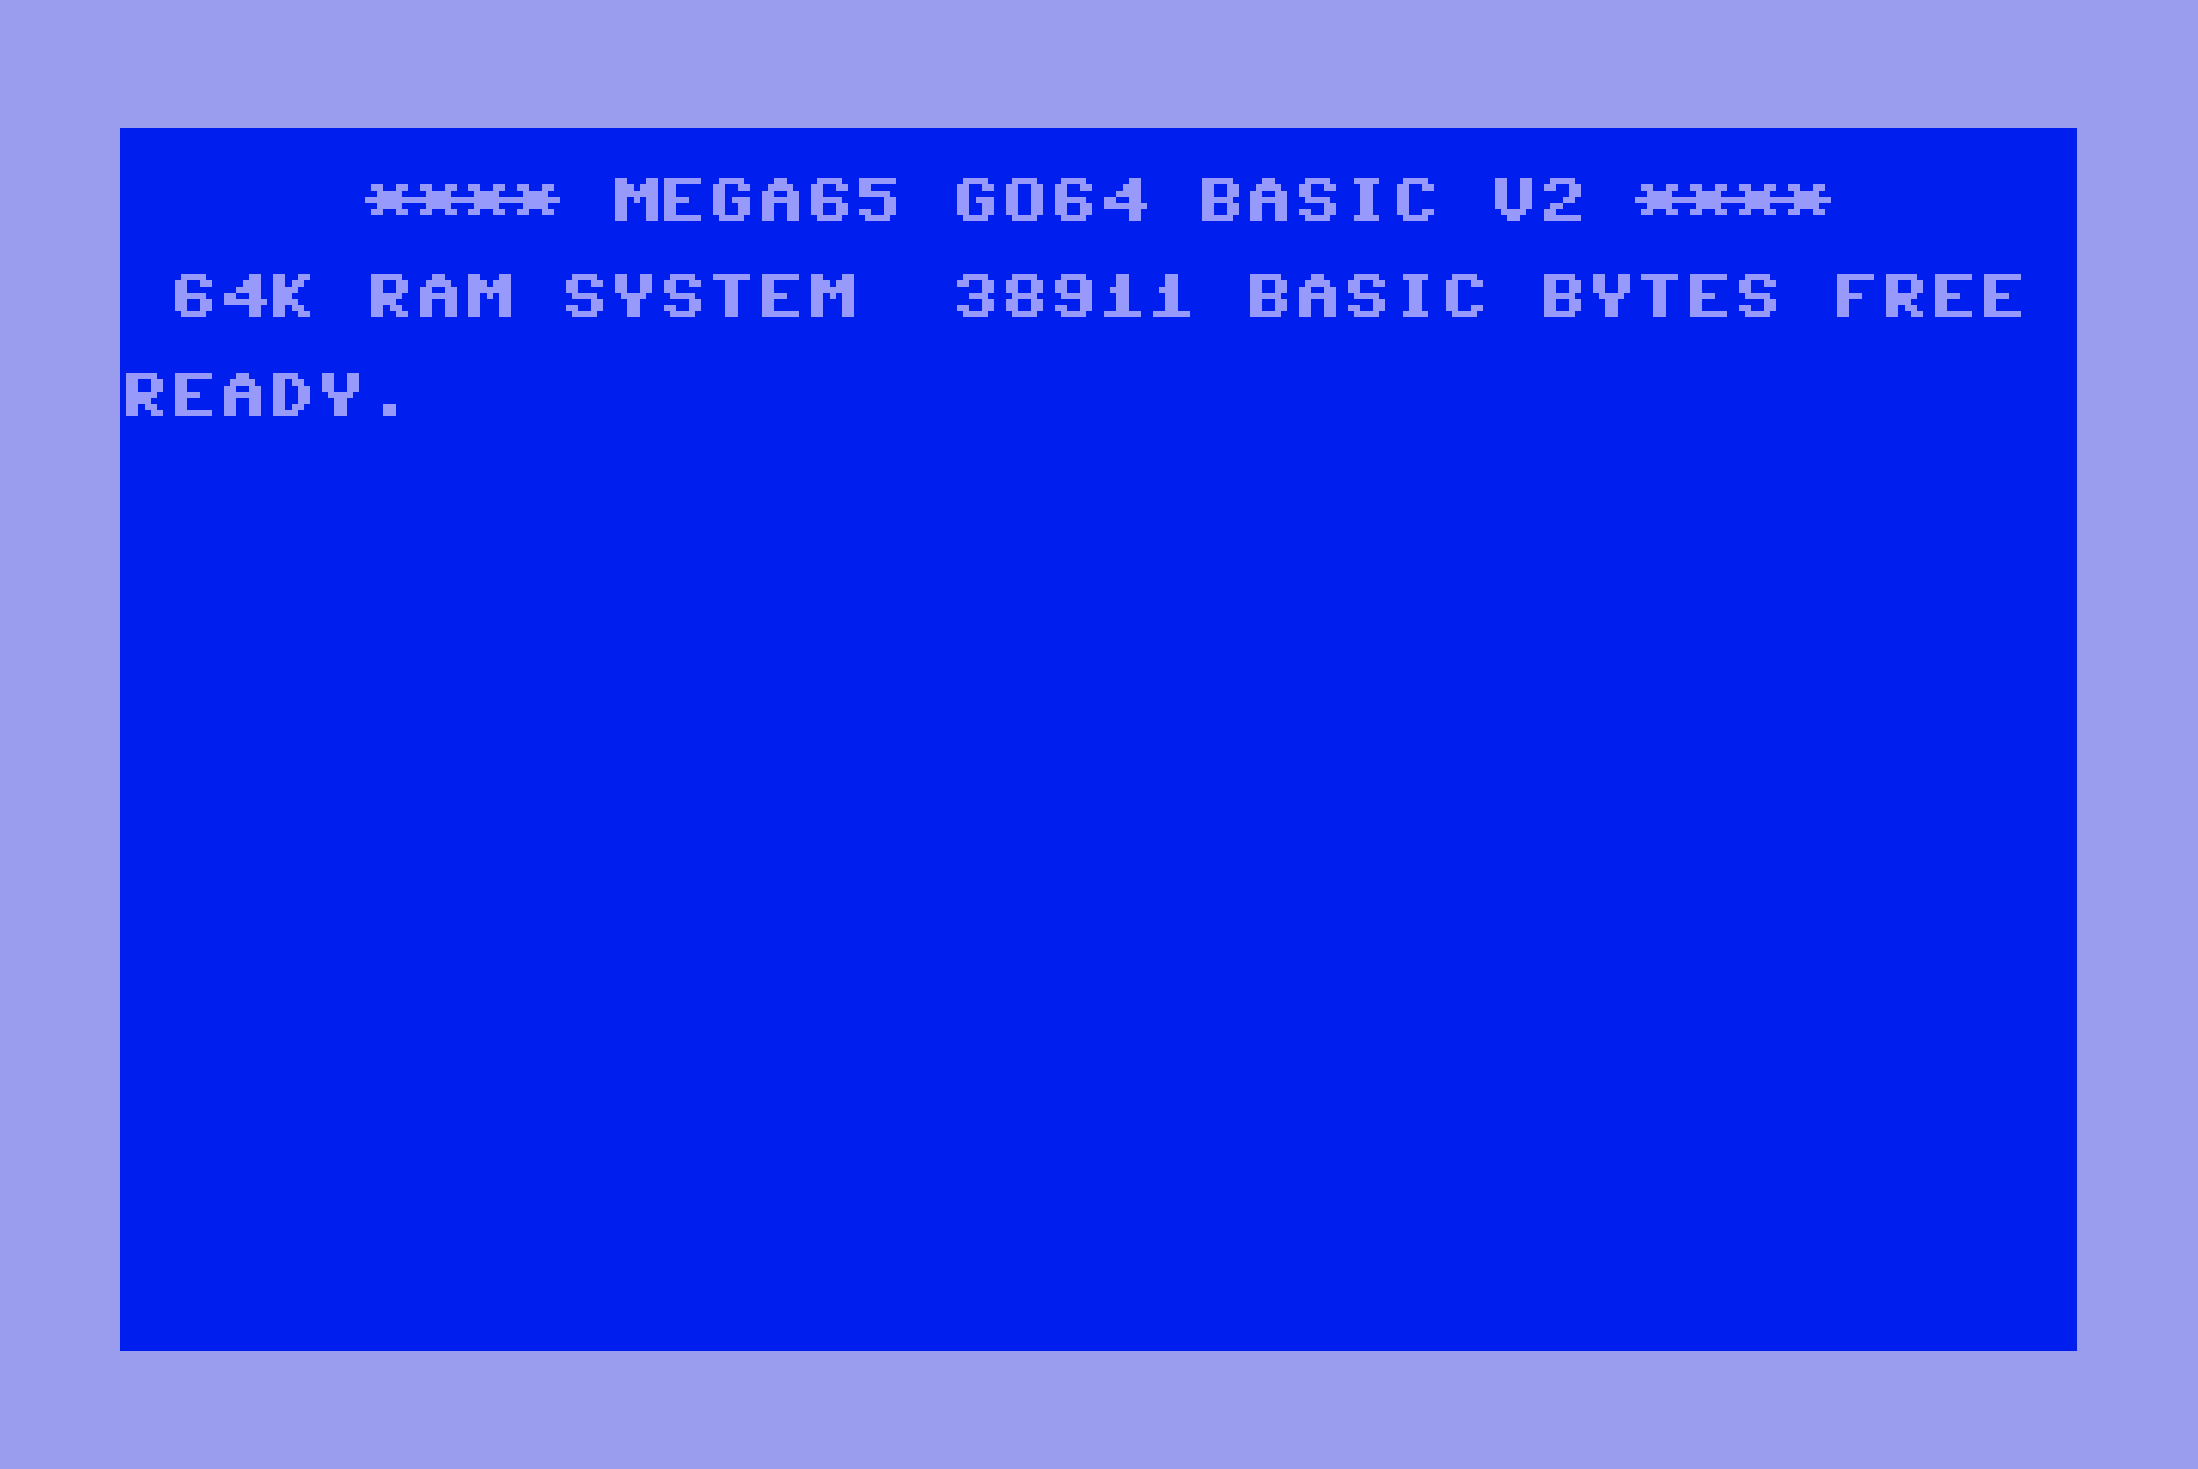
\includegraphics[width=0.7\linewidth]{images/go64.pdf}
\end{center}

De GO64-modus is eigenlijk slechts een tijdelijke herconfiguratie van de MEGA65. Alle voorzieningen van de MEGA65 blijven aanwezig, waaronder het Freezer-menu voor het aankoppelen van D81-schijfimages.

Veel Commodore 64-software is op het internet te vinden in de vorm van D64-schijfimages. De MEGA65 ondersteunt via de SD-kaart en het Freezer-menu uitsluitend D81-schijfimages. U kunt een randapparaat, zoals de SD2IEC,\index{SD2IEC device} op de IEC-poort van de MEGA65 aansluiten om D64-schijfimages te gebruiken. Zorg dat u een SD2IEC aanschaft met een onafhankelijke voeding en niet een exemplaar dat afhankelijk is van een tape-aansluiting van de Commodore 64.\footnote{Zie voor meer informatie over SD2IEC-apparaten: \url{https://www.c64-wiki.com/wiki/SD2IEC}}

\subsection{De FPGA-core ``C64 for MEGA65''}
\index{Core!C64-core}\index{Commodore 64!Core}

De FPGA-core {\it C64 for MEGA65} van MJoergen en sy2002 herschept de oorspronkelijke Commodore 64-computer op de MEGA65-hardware met een hoge mate van nauwkeurigheid. Het doet dit door de MEGA65-core volledig te vervangen door een core die de chipset van de Commodore 64 implementeert, met inbegrip van de CPU. MEGA65-voorzieningen, zoals het Freezer-menu, zijn niet beschikbaar wanneer de C64-core draait. In plaats daarvan biedt de core een eigen menu voor het aankoppelen van D64-schijfimages en andere voorzieningen. Druk op de toets \specialkey{HELP} terwijl de core draait om dit menu te openen.

% TODO: When the cartridge-to-core configuration feature is complete:
% With the C64 core installed, you can configure the MEGA65 boot process to use the core when a Commodore 64 cartridge is connected, instead of using the less-compatible GO64 mode. ...
% (Refer to chapter \vref{cha:cores})

Zie voor informatie over het installeren van FPGA-cores hoofdstuk \vref{cha:cores}. Om de core {\it C64 for MEGA65} te downloaden en de belangrijke installatie-instructies te lezen, zie: \url{https://github.com/MJoergen/C64MEGA65}

\chapter{Configureren van uw MEGA65}

\section{Configureren van uw MEGA65}
\label{cha:configuringyourmega}
\index{Configuratie}

Dit hoofdstuk beschrijft hoe u uw MEGA65 configureert.

Omdat de configuratiegegevens op de SD-kaart worden opgeslagen, beschrijft dit hoofdstuk ook hoe u een nieuwe SD-kaart voorbereidt. Uw MEGA65 wordt met een vooraf geïnstalleerde SD-kaart geleverd. Indien u uw MEGA65 met de vooraf geïnstalleerde SD-kaart configureert en later een nieuwe SD- of microSD-kaart installeert, moet u uw configuratie-instellingen opnieuw instellen.

Dit hoofdstuk laat u tevens kennismaken met de website MEGA65 Filehost, waarmee u games, apps, hulpprogramma's en systeemupdates voor uw computer kunt downloaden.

\section{Configuratiehulpprogramma}
\label{sec:configuration-utility}
\index{Configuratie!Hulpprogramma}

U kunt uw MEGA65 configureren met het Configuratiehulpprogramma. Dit omvat de instellingen die werden weergegeven toen u de computer voor het eerst inschakelde en vele andere.

Om het Configuratiehulpprogramma te openen, schakelt u de MEGA65 uit, houdt u de toets \specialkey{ALT} ingedrukt en schakelt u de MEGA65 weer in. Het hulpprogrammamenu\index{Hulpprogrammamenu} verschijnt met verschillende opties. Druk op \megakey{1} om het Configuratiehulpprogramma te starten.

\begin{center}
  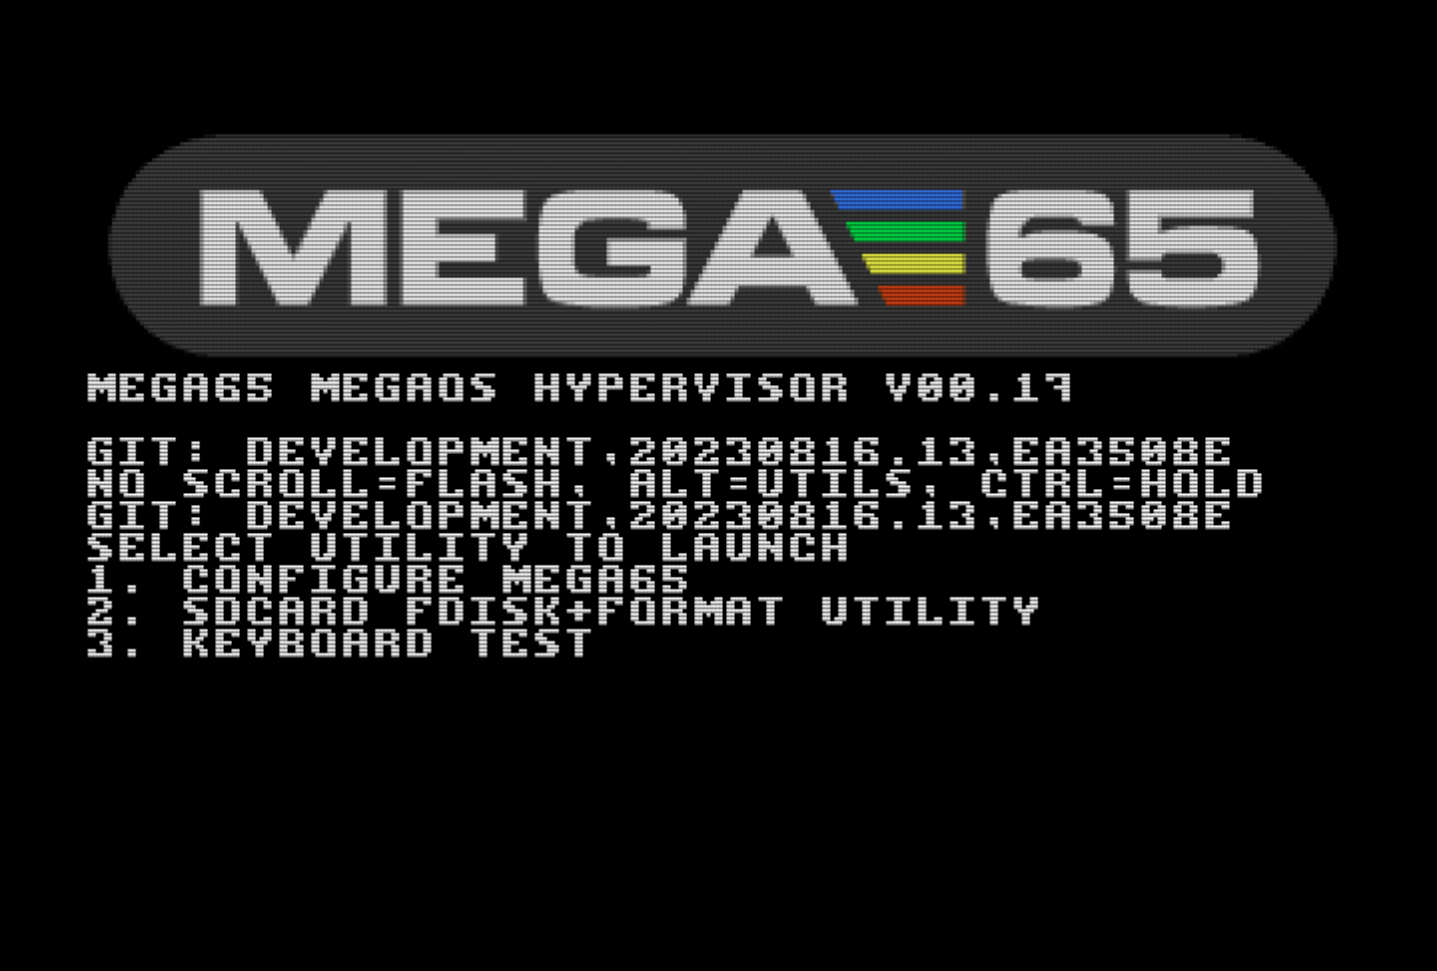
\includegraphics[width=0.7\linewidth]{images/ss-utilmenu.png}
\end{center}

Het Configuratiehulpprogramma bevat verscheidene bladzijden met instellingen, die u kunt doorlopen met het toetsenbord of met een op poort 1 aangesloten muis. Gebruik \megakey{$\leftarrow$} en \megakey{$\rightarrow$} om tussen de bladzijden te bladeren en \megakey{$\uparrow$} en \megakey{$\downarrow$} om onderdelen op een bladzijde te selecteren. Druk op \specialkey{RETURN} of \megakey{SPACE} om een instelling om te schakelen of een waarde te wijzigen.

\subsection{Input}
\index{Configuratie!Muis}

Op de bladzijde {\bf Input} stelt u de muisinstellingen voor de twee randapparaatpoorten in.

\begin{center}
  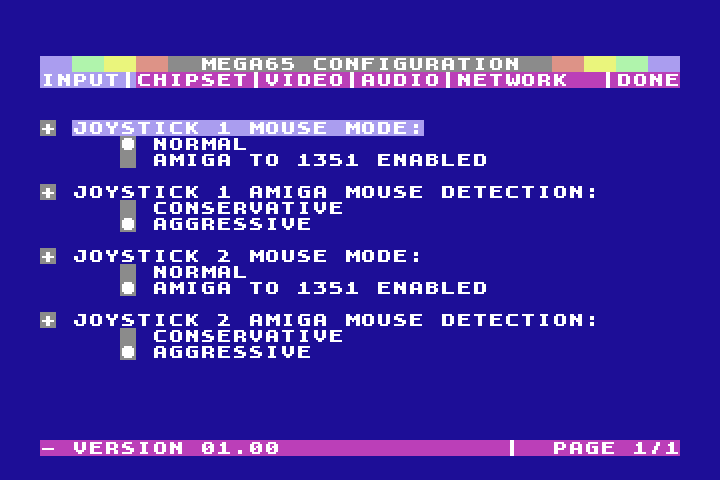
\includegraphics[width=0.7\linewidth]{images/ss-m65config-1.png}
\end{center}

De MEGA65 ondersteunt de Commodore 1351-muis,\index{Commodore 1351-muis} de Commodore Amiga-muis\index{Commodore Amiga-muis} of moderne equivalenten, zoals een USB-muis die met een \href{https://retrohax.net/shop/amiga/mouster/}{mouSTer}-adapter is aangesloten.\index{mouSTer-adapter} De poort moet op het juiste muistype worden ingesteld, waarbij {\bf normal} naar de 1351-muis verwijst. Indien een Amiga-muis is aangesloten terwijl de poort in de modus {\bf normal} staat, kan deze het gedrag van het toetsenbord verstoren.

Met de instelling {\bf 1351 De-jitter} stelt u de gevoeligheid in de Commodore 1351-muismodus af om jitter van het muispijltje te voorkomen. Het wordt aanbevolen deze op {\bf on} te laten staan wanneer u in de modus {\bf normal} een 1351-muis gebruikt.

\subsection{Chipset}
\index{Configuratie!Opstartschijf}

Op de bladzijde {\bf Chipset} stelt u verschillende functies in, waaronder de real-time klok.

\begin{center}
  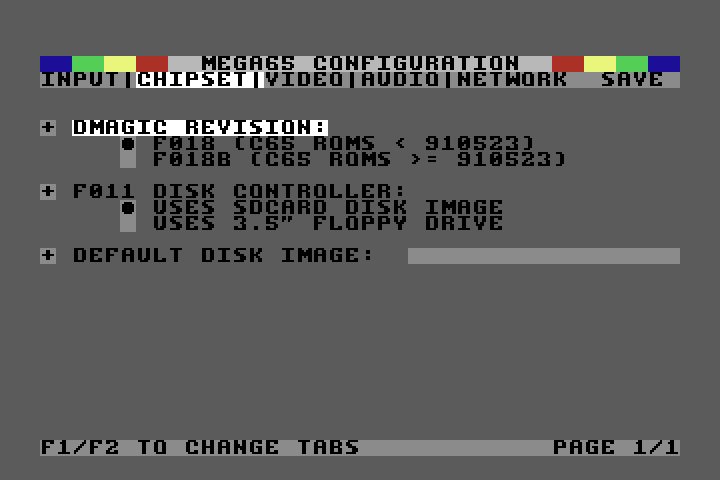
\includegraphics[width=0.7\linewidth]{images/ss-m65config-2.png}
\end{center}

Om de real-time klok in te stellen, selecteert u het tijd- of datumveld, typt u de volledige waarde en drukt u vervolgens op \specialkey{RETURN}.\index{Real-time klok!Datum/tijd instellen}\index{Configuratie!Real-time klok} De klokinstelling wordt pas van kracht wanneer u op \specialkey{RETURN} drukt; zonder \specialkey{RETURN} wijzigt er niets. Merk op dat alle overige instellingen pas aan het einde worden opgeslagen. Alleen de RTC wordt onmiddellijk bijgewerkt.

Het veld {\bf DMAGIC revision} bepaalt het gedrag van de DMA-controller. In de meeste gevallen wilt u de nieuwere instelling {\bf F018B} gebruiken. De instelling {\bf F018} dient voor achterwaartse compatibiliteit wanneer de C65-versies van de ROM worden gebruikt en is niet altijd vereist.

Het veld {\bf F011 disk controller}\index{F011-schijfcontroller} bepaalt of de MEGA65 bij het inschakelen van de computer een opstartschijf zoekt op de SD-kaart of in het fysieke 3.5 inch-diskettestation.\index{Configuratie!Opstartschijf} Wanneer deze op {\bf SDCARD disk image,} is ingesteld, gebruikt de MEGA65 het virtuele D81-schijfimage dat in het veld {\bf default disk image} is vermeld als opstartschijf. Wanneer u uw MEGA65 voor het eerst ontvangt, is dit ingesteld op de Intro Disk,\index{Intro Disk} genaamd {\tt MEGA65.D81}. U kunt dit wijzigen naar een andere schijf. Om het automatisch koppelen uit te schakelen, wijzigt u de schijfnaam in een bestandsnaam die niet bestaat, of hernoemt u het bestand {\tt MEGA65.D81} op de SD-kaart. (Indien u het veld leeg laat, wordt standaard {\tt MEGA65.D81} gebruikt.)

Indien {\bf F011 disk controller} op {\bf 3.5" floppy drive,} is ingesteld, pauzeert het opstartproces vlak vóór de \screentext{READY}-prompt om te controleren of er een opstartschijf in het station is geplaatst. Indien u geen fysieke opstartschijf gebruikt, kunt u deze op {\bf SDCARD disk image} laten staan voor een sneller opstartproces.

{\bf Long FN support} verwijst naar de ondersteuning van lange bestandsnamen in de bestandsbrowser van de MEGA65 voor SD-kaarten. Laat deze functie ingeschakeld, tenzij er problemen optreden bij het lezen van bestanden met bestandsnamen die langer zijn dan 11 tekens.

\subsection{Video}
\index{Configuratie!Video}

Op de bladzijde {\bf Video} stelt u de video-instellingen in. Dit zijn dezelfde instellingen als die van de initiële configuratie (``on-boarding''), waaronder de PAL- of NTSC-videomodus, het Digital Video-geluid en CRT-emulatie.\index{Configuratie!Introductie}\index{Scherm!PAL/NTSC instellen}

\begin{center}
  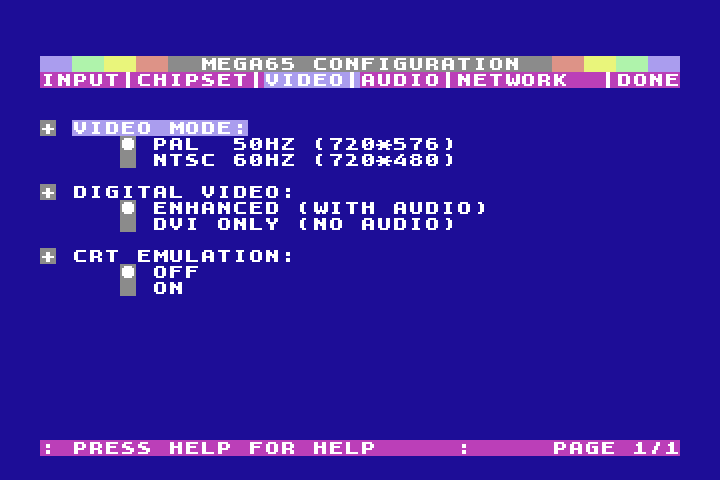
\includegraphics[width=0.7\linewidth]{images/ss-m65config-3.png}
\end{center}

Met {\bf Video mode} kiest u tussen de PAL-compatibiliteitsmodus en de NTSC-compatibiliteitsmodus. U kunt deze instelling ook tijdens het uitvoeren van programma's wijzigen met het Freezer-menu.

Met de instelling {\bf Digital Video} schakelt u het gecombineerde video- en audiosignaal over de Digital Video-poort in of uit. Indien uw Digital Video-beeldscherm ingebouwde luidsprekers heeft, schakelt u deze instelling in ({\bf Enhanced (with audio)}) om deze te gebruiken. Sommige DVI-beeldschermen zonder ingebouwde luidsprekers vereisen dat deze instelling wordt uitgeschakeld.

{\bf CRT emulation} is een optionele instelling die het beeld meer laat lijken op dat van een klassiek beeldbuismonitor wanneer u een modern plat beeldscherm gebruikt.

\subsection{Audio}
\index{Configuratie!Audio}

Op de bladzijde {\bf Audio} stelt u het geluidssysteem van de MEGA65 in.\index{Configuratie!Audio} In de meeste gevallen kunt u deze instellingen op hun standaardwaarden laten staan.

\begin{center}
  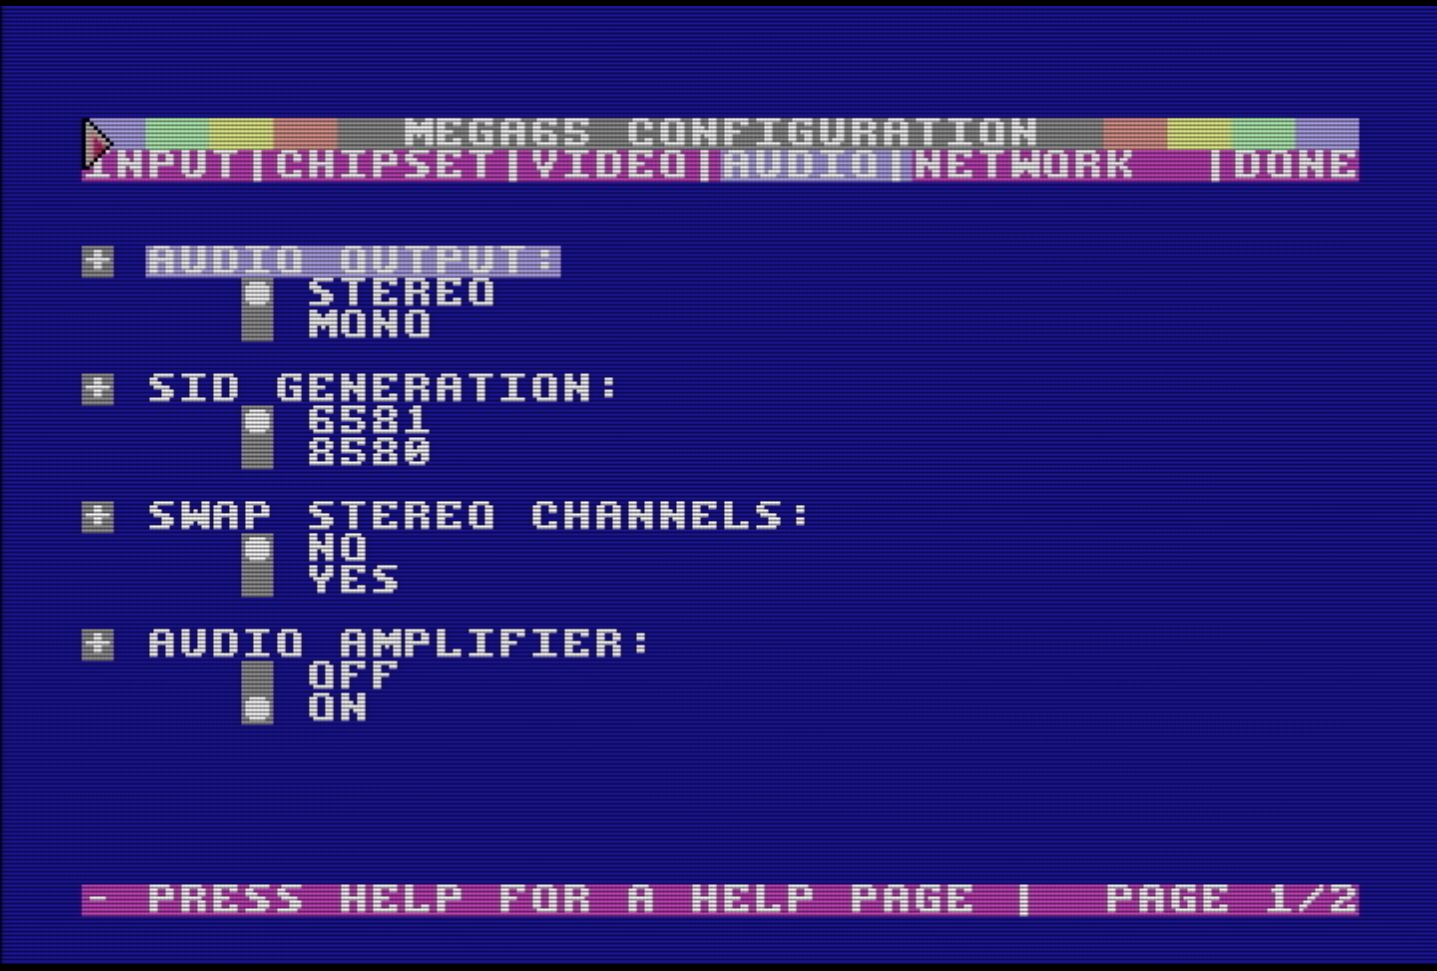
\includegraphics[width=0.7\linewidth]{images/ss-m65config-4.png}
\end{center}

{\bf Audio output} kan worden ingesteld op volledige stereo of op het verzenden van een monauraal signaal naar beide luidsprekers. In de stereomodus kunt u de diverse audioapparaten van de MEGA65 met de audiomixer in het Freezer-menu naar links of rechts in het stereobeeld verplaatsen. De standaardinstellingen plaatsen de vier SID-chips enigszins naar links en rechts.

{\bf SID generation} kiest tussen de audio-emulatie van de twee modellen SID-geluidschips: de oorspronkelijke 6581 die in sommige Commodore 64's wordt gebruikt en de nieuwere 8580 die in latere Commodore 64's en 128's wordt gebruikt. Sommige Commodore 64-spellen maakten gebruik van gebreken in de 6581 die in de 8580 zijn opgelost en klinken daardoor beter met de oudere generatie.

{\bf Swap stereo channels} laat de linker- en rechterluidsprekers van elkaar verwisselen.

{\bf Audio amplifier} regelt de ingebouwde versterker op de 3.5 mm-audioaansluiting. Stel deze in op {\bf on} wanneer u een hoofdtelefoon of een ander apparaat gebruikt dat een versterkt signaal verwacht. Stel deze in op {\bf off} voor een signaal op lijnniveau.

\subsection{Network}
\index{Configuratie!Netwerk}

Op de bladzijde {\bf Network} kunt u het MAC-adres van de ethernetpoort aanpassen. De MEGA65 heeft geen door de hardware toegewezen MAC-adres. In plaats daarvan gebruikt de computer de hier ingevoerde waarde.

Indien het MAC-adres geheel uit nullen bestaat, drukt u op de toets \megakey{R} om een willekeurig adres te genereren. Met een MAC-adres dat geheel uit nullen bestaat, werken netwerkfuncties niet.\index{Configuratie!MAC-adres}\index{Netwerk!MAC-adres}

\begin{center}
  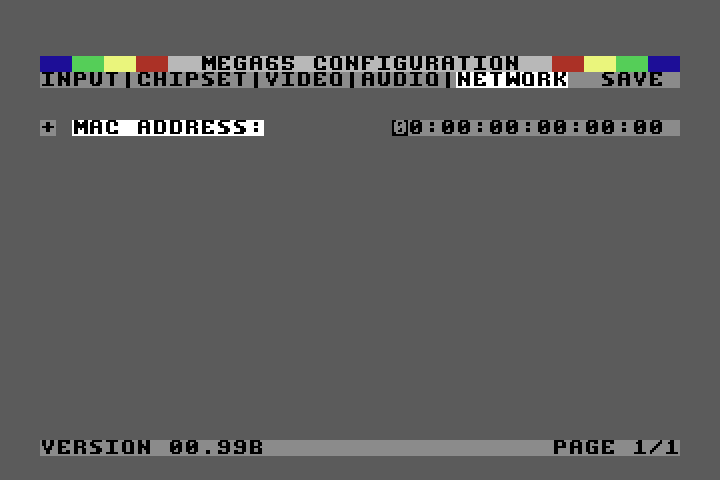
\includegraphics[width=0.7\linewidth]{images/ss-m65config-5.png}
\end{center}

\subsection{Done}

Op de bladzijde {\bf Done} kunt u het Configuratiehulpprogramma verlaten. Indien u wijzigingen hebt aangebracht die u wilt behouden, selecteert u {\bf Save as defaults and exit.} U kunt de wijzigingen ook verwerpen, de fabrieksinstellingen herstellen of volledig opnieuw opstarten naar het scherm van de initiële configuratie.

\begin{center}
  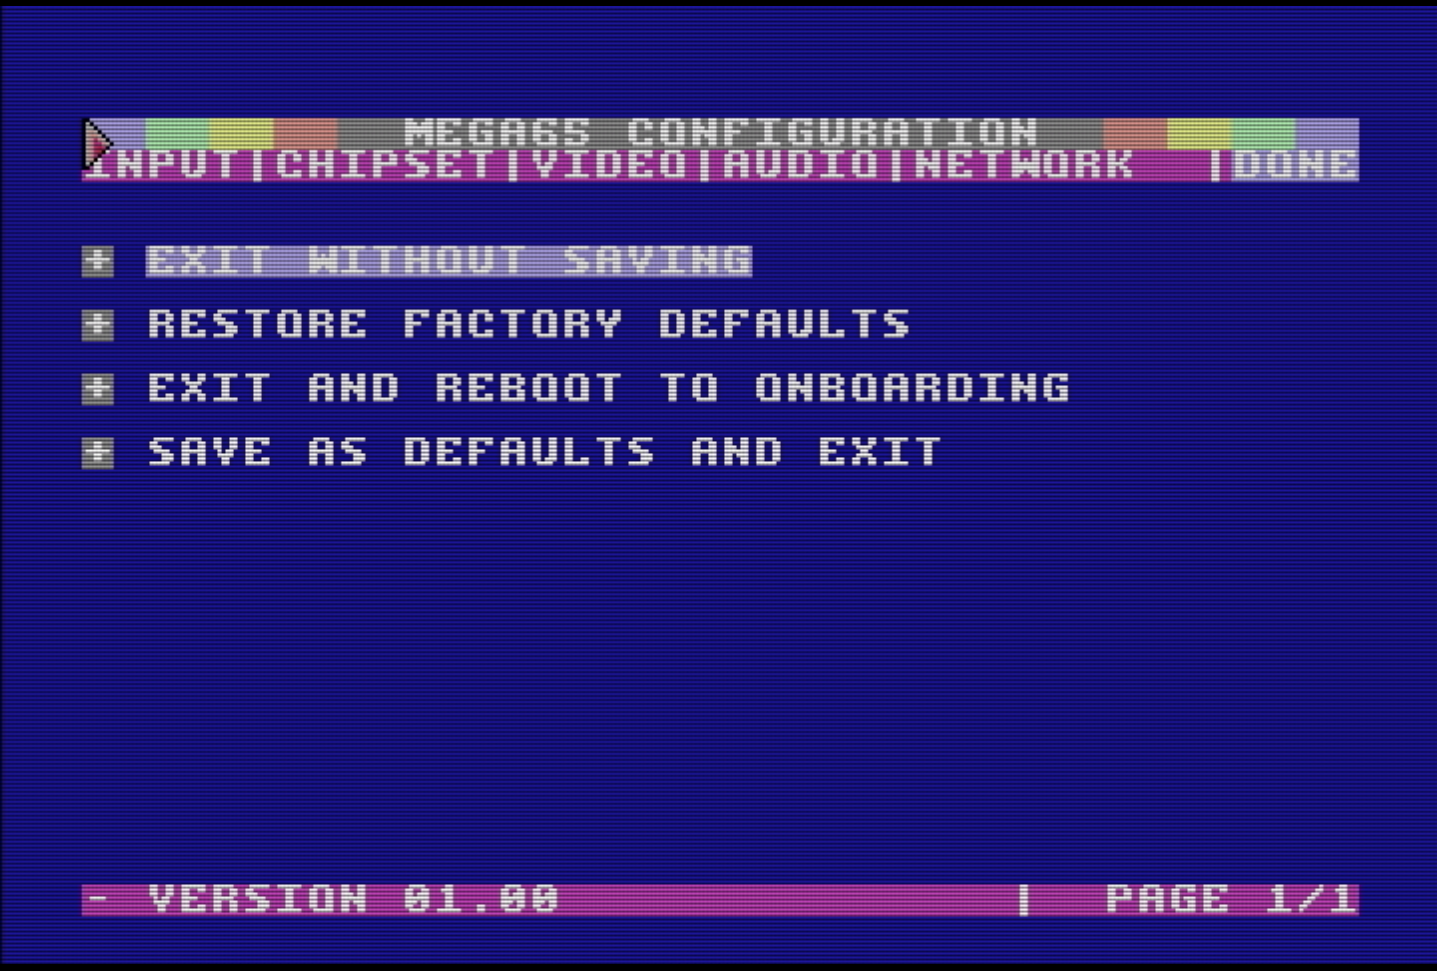
\includegraphics[width=0.7\linewidth]{images/ss-m65config-save.png}
\end{center}

Wanneer u het Configuratiehulpprogramma verlaat, wordt u gevraagd de computer uit en weer in te schakelen. Schakel de computer uit en vervolgens weer in.

\section{Kennismaken met SD-kaarten}
\label{sec:introducing-sd-cards}
\index{SD-kaarten}
\nopagebreak
Uw MEGA65 is uitgerust met twee SD-kaartsleuven: een SD-kaartsleuf op vol formaat in de behuizing, bereikbaar via de onderzijde van de computer, en een microSD-kaartsleuf aan de achterzijde van de computer.\index{SD-kaarten!Locaties} De MEGA65 gebruikt de SD-kaart voor het opslaan van configuratie-instellingen, het laden van het besturingssysteem, het bijwerken van de firmware en het opslaan van uw programmatuur en gegevens als virtuele schijfimages.

De MEGA65 wordt geleverd met een SD-kaart op vol formaat in de interne SD-kaartsleuf, vooraf gevuld met de bestanden van het besturingssysteem en de meegeleverde programmatuur.\footnote{U kunt de oorspronkelijke inhoud van de SD-kaart opnieuw aanmaken met bestanden die u van het internet kunt downloaden. Desondanks wilt u wellicht een reservekopie van de inhoud van de SD-kaart op uw PC maken.} U kunt uw MEGA65 aansluiten en er direct mee beginnen, zonder een nieuwe SD-kaart in te stellen. U kunt deze SD-kaart op zijn plaats laten en doen alsof hij er niet is, alsof uw MEGA65 een computer uit de jaren negentig is met een verborgen mogelijkheid om niet-vluchtige gegevens op te slaan.

De MEGA65 gebruikt slechts één van de twee SD-kaartsleuven tegelijk. Indien er een microSD-kaart in de sleuf aan de achterzijde zit, wordt de interne SD-kaart genegeerd. Welke sleuf u gebruikt, hangt af van het beoogde gebruik van de computer. Naarmate u meer vertrouwd raakt met uw MEGA65, wilt u de SD-kaart wellicht tussen de MEGA65 en uw PC verplaatsen om bestanden te kopiëren en systeemupdates uit te voeren. Dit is gemakkelijker met de externe microSD-kaartsleuf.

U kunt uw MEGA65 ook met een ethernetkabel op uw PC of het plaatselijke netwerk aansluiten en met een hulpprogramma bestanden tussen de twee computers overbrengen. De bestandsoverdrachtfunctie heeft toegang tot de bestanden op de SD-kaart en gebruikt de sleuf die op dat moment actief is. Zie voor meer informatie over het overbrengen van bestanden hoofdstuk \vref{cha:transferring-files}.

\section{Een nieuwe SD-kaart voorbereiden}

U kunt de microSD-kaartsleuf aan de achterzijde van de MEGA65 gebruiken als permanente opslagruimte voor de configuratie- en systeembestanden van de computer. Een voorbereide kaart in deze sleuf heeft voorrang op de SD-kaart die in de computer is geïnstalleerd. Het is handig om een microSD-kaart geïnstalleerd te hebben indien u de kaart tussen uw MEGA65 en uw PC wilt verplaatsen.

De volgende aanwijzingen gelden voor geheugenkaarten in zowel de externe microSD-kaartsleuf als de interne SD-kaartsleuf op vol formaat.

De MEGA65 ondersteunt SD-kaarten van het type SDHC, met een grootte tussen 4GB en 32GB. Oudere kaarten kleiner dan 4GB en nieuwere SDXC-kaarten groter dan 32GB zullen naar verwachting niet werken.

Een SD-kaart moet vóór gebruik door de MEGA65 worden voorbereid met behulp van het SD-kaarthulpprogramma.\index{SD-kaarthulpprogramma} Het hulpprogramma maakt twee partities aan: een verborgen partitie voor configuratiegegevens en freezergegevens en een FAT32-compatibele partitie voor schijfimages en systeembestanden. U kunt toegang krijgen tot de FAT32-partitie door de SD-kaart op uw PC aan te sluiten.\footnote{Indien u een reservekopie van de volledige SD-kaart inclusief de verborgen partitie wilt maken, moet u een schijfhulpprogramma gebruiken dat volledige partities kopieert en niet alleen de bestanden op de FAT32-partitie.}

Een SD-kaart die door een andere computer is geformatteerd, werkt {\em niet} met de MEGA65, zelfs indien die computer alleen de FAT32-partitie wist. U {\em moet} de SD-kaart formatteren met het SD-kaarthulpprogramma van de MEGA65.

\subsection{De SD-kaart plaatsen}

Het formatteren van een SD-kaart wist de inhoud en deze handeling kan niet ongedaan worden gemaakt. Wij raden u aan de interne SD-kaart die bij de computer is geleverd niet te wissen.

Het SD-kaarthulpprogramma vraagt u welke van de kaarten die momenteel in de computer zijn geplaatst, geformatteerd moet worden. U kunt er als voorzorgsmaatregel voor kiezen de interne SD-kaart te verwijderen voordat u het SD-kaarthulpprogramma opent. U kunt hem later opnieuw plaatsen of hem uit de computer laten totdat u hem nodig hebt. Dit is tevens een goede gelegenheid om de gebundelde softwarebestanden (met bestandsnamen die eindigen op {\tt .D81}) van de interne SD-kaart naar uw PC te kopiëren, zodat u ze later op de nieuwe SD-kaart kunt kopiëren.

Het hulpprogrammamenu is toegankelijk, zelfs indien er geen geldige SD-kaart aanwezig is. U kunt een nieuw systeem opstarten met uitsluitend een geschikte SD-kaart en het SD-kaarthulpprogramma.

Plaats de SD-kaart die u wilt voorbereiden, voordat u verdergaat.

\subsection{Het SD-kaarthulpprogramma}
\index{SD-kaarthulpprogramma}

U opent het SD-kaarthulpprogramma vanuit het hulpprogrammamenu.\index{Hulpprogrammamenu} Schakel de MEGA65 uit, houd de toets \specialkey{ALT} ingedrukt en schakel hem weer in. Selecteer in het menu optie \megakey{2} om het SD-kaarthulpprogramma te starten (\texttt{SDCARD FDISK+FORMAT UTILITY}).

\begin{center}
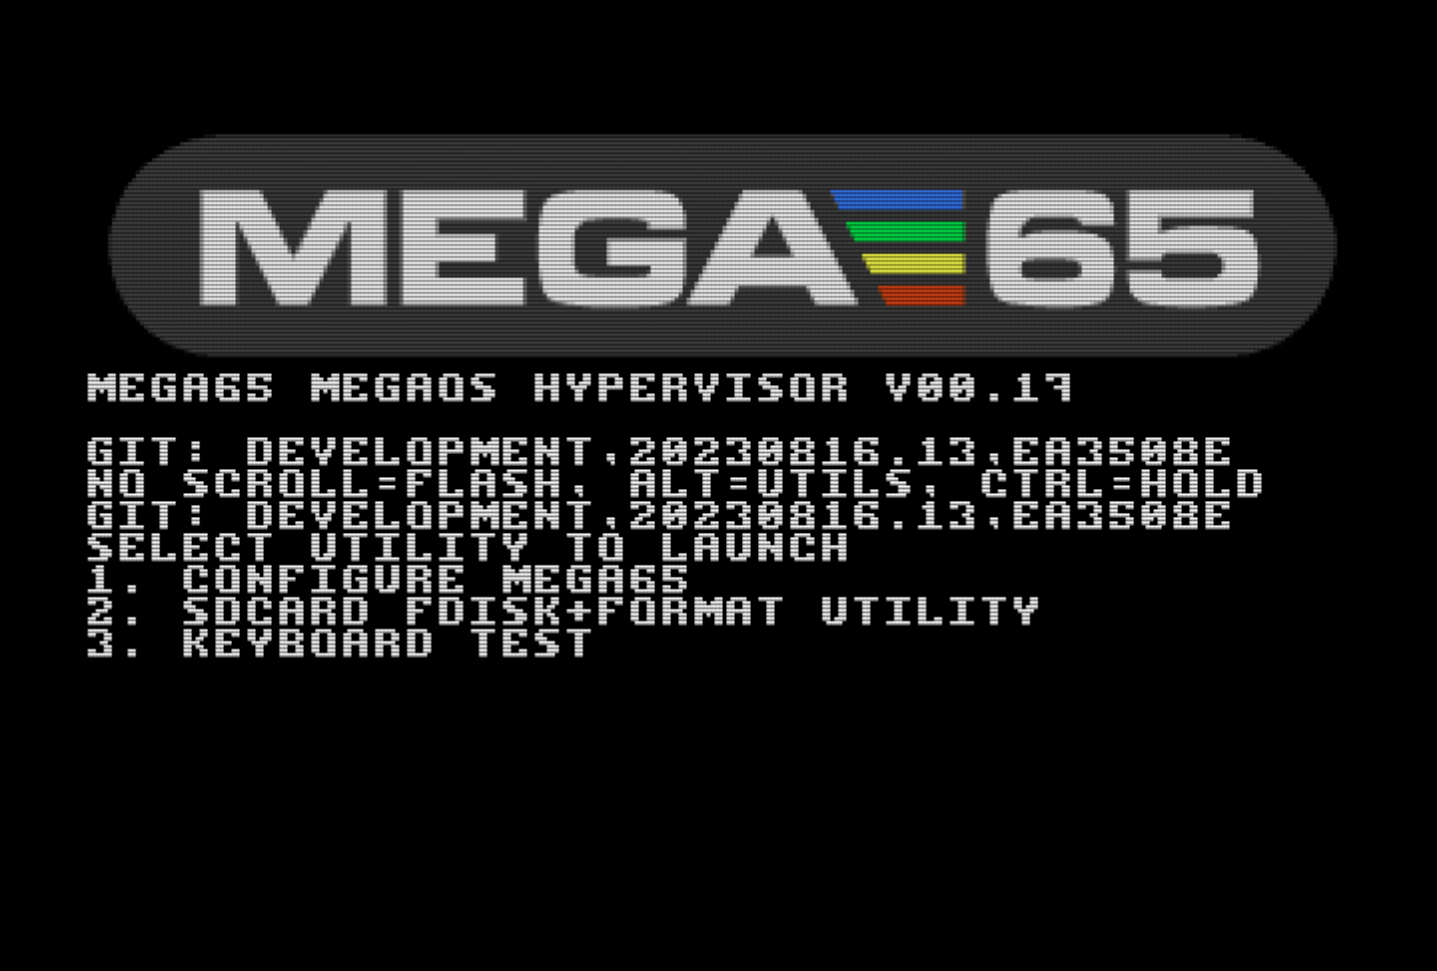
\includegraphics[width=0.7\textwidth]{images/ss-utilmenu.png}
\end{center}

Het SD-kaarthulpprogramma opent en zoekt naar SD-kaarten die in de sleuven zijn geïnstalleerd. Indien u de SD-kaart die u wilt voorbereiden nog niet hebt geplaatst, doe dat nu en druk daarna op \megakey{R} om opnieuw te scannen.

\begin{center}
  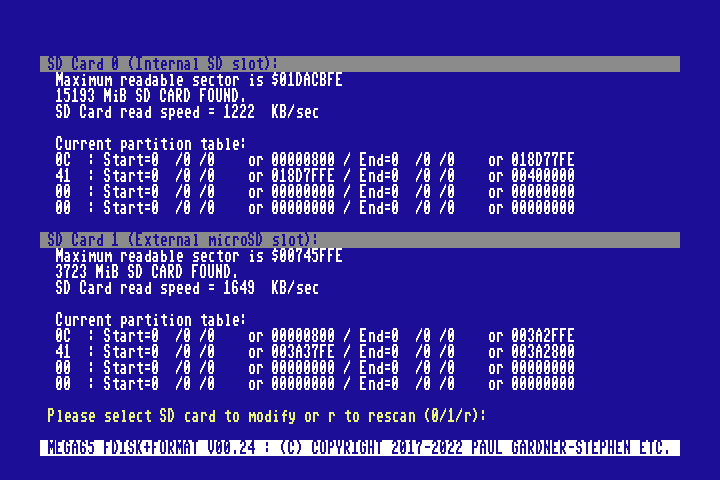
\includegraphics[width=0.7\textwidth]{images/ss-m65fdisk-busselect.png}
\end{center}

Selecteer de kaart die u wilt voorbereiden: \megakey{0} voor de interne SD-kaart, \megakey{1} voor de externe microSD-kaart. Indien er twee kaarten zijn geïnstalleerd, {\em let er goed op dat u de juiste kaartsleuf kiest.}

Het SD-kaarthulpprogramma vraagt bevestiging voordat de SD-kaart wordt gewist. Als allerlaatste voorzorgsmaatregel moet u de tekst {\tt DELETE EVERYTHING} in hoofdletters typen en vervolgens op \specialkey{RETURN} drukken om door te gaan. (Indien u dit proces wilt afbreken, is het veilig om de MEGA65 op dit moment uit te schakelen.)

\begin{center}
  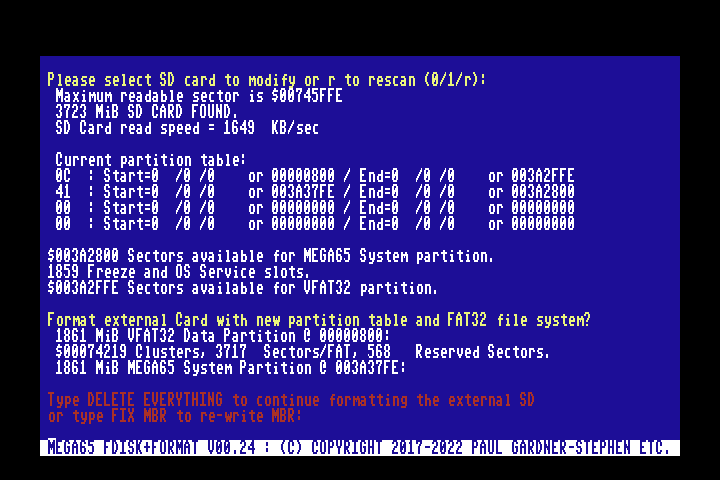
\includegraphics[width=0.7\textwidth]{images/ss-m65fdisk-typesomething.png}
\end{center}

Het hulpprogramma wist de SD-kaart en maakt de partities aan. Wanneer het klaar is, vraagt het of u de systeembestanden wilt installeren. De systeembestanden (met bestandsnamen die eindigen op {\tt .M65} en {\tt .ROM}) zijn in de core ingebed en worden naar de FAT32-partitie gekopieerd voor gebruik. Indien u een bijgewerkte MEGA65-core in slot 1 hebt geïnstalleerd, selecteert u deze; selecteert u anders de in de fabriek geïnstalleerde MEGA65-core in slot 0. (Indien u uw MEGA65 zojuist hebt ontvangen, is slot 0 de enige optie.)

\begin{center}
  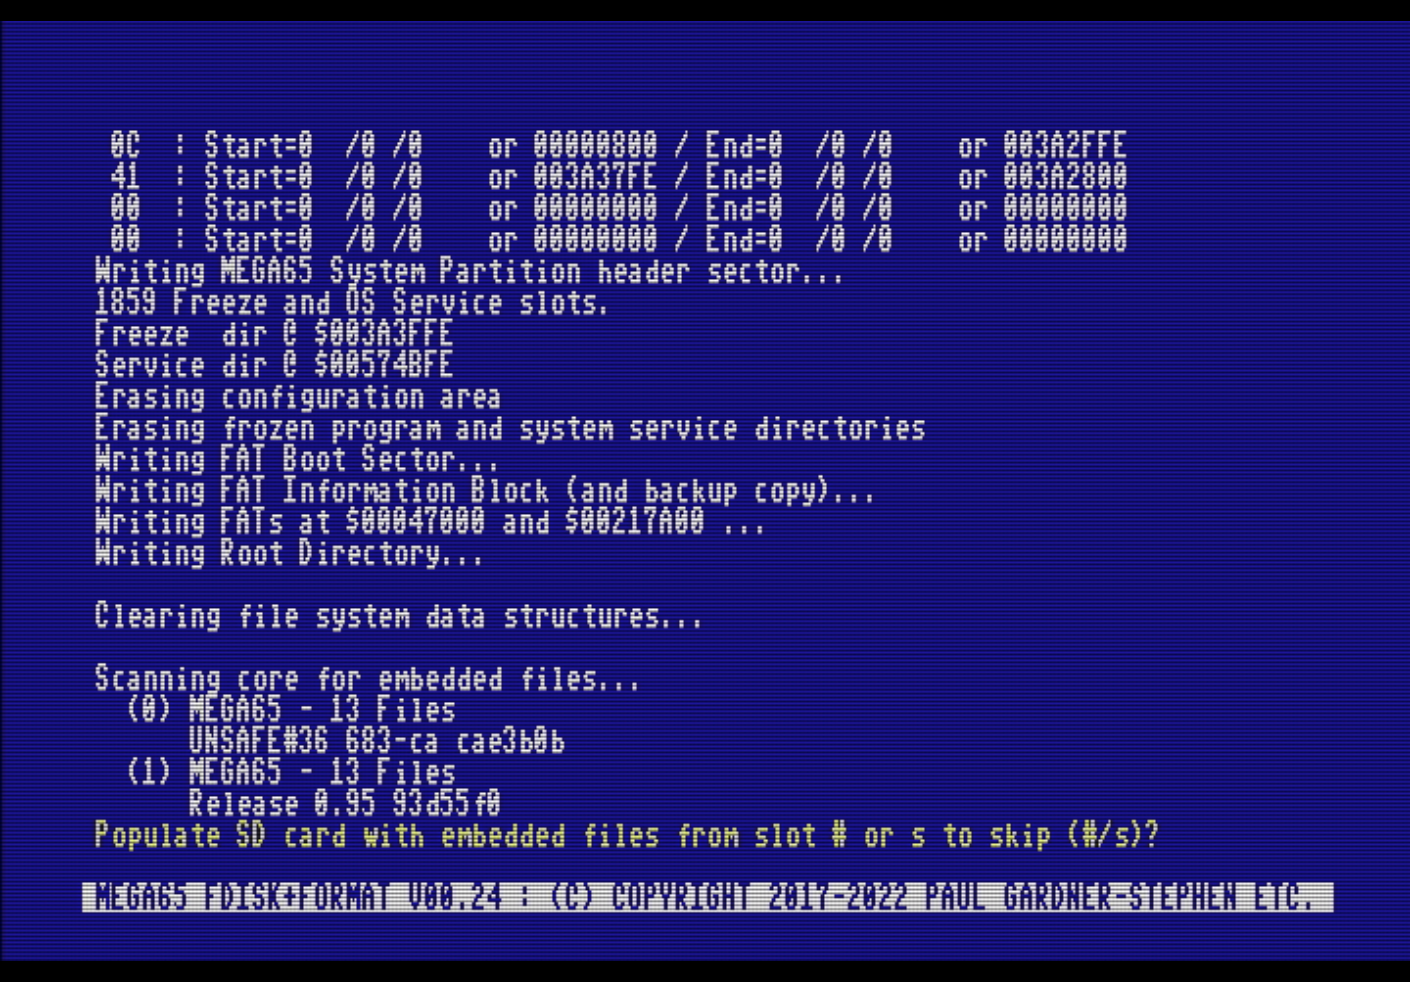
\includegraphics[width=0.7\textwidth]{images/ss-m65fdisk-populate.png}
\end{center}

Start de computer opnieuw op wanneer daarom wordt gevraagd.\footnote{Indien u een core selecteert die {\tt MEGA65.ROM} niet als één van de ingebedde bestanden bevat, vraagt het hulpprogramma u de SD-kaart naar uw PC te verplaatsen om dit bestand erop te kopiëren. Dit gebeurt alleen wanneer u een MEGA65-core gebruikt die afkomstig is van een andere bron dan een officieel MEGA65-releasespakket. Zie voor meer informatie over cores en het verkrijgen van {\tt MEGA65.ROM} hoofdstuk \vref{cha:cores}.}

\subsection{De gebundelde programmatuur verkrijgen}

De systeembestanden die naar de vers geformatteerde SD-kaart worden gekopieerd, omvatten niet de gebundelde programmatuur die bij de oorspronkelijke SD-kaart in de interne kaartsleuf werd meegeleverd. U kunt deze bestanden met uw PC van de oorspronkelijke SD-kaart kopiëren en ze daarna op de nieuwe SD-kaart kopiëren.

De website MEGA65 Filehost\index{Filehost-website} biedt allerlei bestanden aan die u voor uw MEGA65 kunt downloaden. Dit omvat de nieuwste versies van de platformcomponenten, alternatieve cores en honderden spellen, demo's en toepassingen die door de MEGA65-gemeenschap zijn gemaakt. Dit omvat tevens de gebundelde programmatuur van de oorspronkelijke SD-kaart die bij de computer werd meegeleverd.

Indien u de gebundelde softwarebestanden niet meer hebt, kunt u ze verkrijgen via de website MEGA65 Filehost. Bezoek de volgende URL:

\url{https://files.mega65.org/?id=all-intros-public}

\chapter{De MEGA65 upgraden}

\section{Hoe u een MEGA65 kunt upgraden}
\label{cha:cores}

Het MEGA65-platform bestaat uit drie belangrijke onderdelen:

\begin{enumerate}
  \item De {\bf MEGA65-core},\index{Core} een beschrijving van de chipset die op de FPGA draait  \item De {\bf ROM},\index{ROM} code die het besturingssysteem in Commodore-stijl (KERNAL) en BASIC definieert  \item {\bf Systeemsoftware} voor functies zoals het Freezer-menu\index{Freezer-menu}
\end{enumerate}

U kunt deze onderdelen upgraden zodra er nieuwe versies verschijnen. U kunt ook één of meer van deze onderdelen afzonderlijk vervangen. Bij de core en de ROM kunt u zelfs meerdere versies tegelijk geïnstalleerd hebben en daartussen schakelen. In plaats van de nieuwste MEGA65-ROM kunt u bijvoorbeeld overschakelen naar de originele prototype-ROM van de Commodore 65. Of u kunt overschakelen naar een andere core die ervoor zorgt dat uw MEGA65-hardware zich geheel als een andere computer gedraagt, zoals een Commodore 64 of een ZX Spectrum.

De ROM en de systeemsoftware zijn bestanden die op de SD-kaart staan; het upgraden ervan is even eenvoudig als het vervangen van de bestanden. Om de core te upgraden installeert u via een bepaald proces een core-bestand in het core-flashgeheugen van de MEGA65. Dit hoofdstuk beschrijft dit proces.

\subsection{Wat is een core?}
\index{Core!Wat is een core?}

De hardware-architectuur van de MEGA65 is gebaseerd op een veelzijdige chip die een ``Field Programmable Gate Array'' of FPGA wordt genoemd.\index{Field Programmable Gate Array (FPGA)} Dit is een speciaal soort computerchip die geprogrammeerd kan worden om zich als andere chips voor te doen. Het doet dit door een enorme reeks logische poorten zodanig te configureren dat de poorten schakelingen nabootsen. FPGA's zijn geen emulatie, maar een elektronische nabootsing van andere chips. FPGA-code wordt soms aangeduid als {\em firmware,} een term die u wellicht herkent van moderne computers en andere apparaten.

Uw MEGA65 is in de fabriek geprogrammeerd om een chipset na te bootsen die is gebaseerd op de originele Commodore 65 en door het MEGA65-team is ontworpen. U kunt de FPGA van de MEGA65 opnieuw programmeren om te upgraden naar nieuwe versies van de MEGA65-chipset of om de chipset te vervangen door die van een heel andere computer!

Elke mogelijke chipset wordt een {\em core} genoemd. De MEGA65 kan maximaal acht cores opslaan en u kunt tussen deze cores schakelen via een menu dat opent wanneer u de computer inschakelt. U kunt dit menu ook gebruiken om een nieuwe core vanaf een bestand op de SD-kaart te laden, een proces dat {\em flashen} heet.

Leden van de MEGA65-gemeenschap hebben diverse nuttige en leuke alternatieve cores voor de FPGA-hardware gemaakt. \href{https://github.com/MJoergen/C64MEGA65}{{\em C64 voor MEGA65}} van MJoergen en sy2002 bootst de originele Commodore 64-computer met een hoge mate van nauwkeurigheid na en is perfect voor het uitvoeren van Commodore 64-spellen, demo's en toepassingen. Andere cores bootsen de ZX Spectrum, de Game Boy en zelfs de hardware van de originele Galaga-arcademachine na. De FPGA van de MEGA65 is krachtig genoeg om vrijwel alle 8-bit-homecomputers na te bootsen en waarschijnlijk ook enkele 16-bit-computers en spelcomputers, zoals de Commodore Amiga. Het hardware-ontwerp van de MEGA65, de indeling van het moederbord, de FPGA-core en overige informatie zijn allemaal gratis beschikbaar onder diverse openbronlicenties, zodat iedereen vrij is andere cores voor de MEGA65-hardware te maken.

\section{De versies van de onderdelen bepalen}
\label{sec:versions}

Alle onderdelen van het MEGA65-platform hebben een versieaanduiding. De MEGA65 kan de versieaanduidingen van al zijn onderdelen weergeven met het MEGA65-informatiehulpprogramma.\index{MEGA65-informatiehulpprogramma}

Om het MEGA65-informatiehulpprogramma te openen:

\begin{enumerate}
  \item Schakel de MEGA65 in en laat hem opstarten tot BASIC.  \item Open de Freezer:\index{Freezer-menu} houd \widekey{RESTORE} één seconde ingedrukt en laat hem daarna los.  \item Druk op \specialkey{HELP}. Het MEGA65-informatiehulpprogramma opent.
\end{enumerate}

\begin{center}
  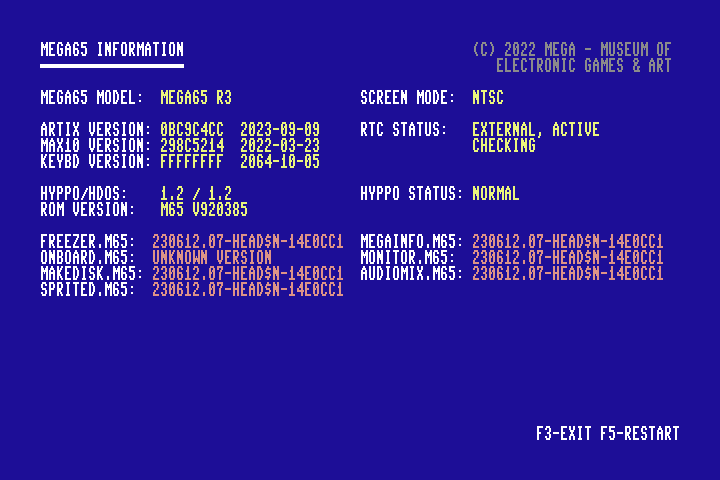
\includegraphics[width=0.7\linewidth]{images/megainfo.png}
\end{center}

Noteer deze versieaanduidingen:
\nopagebreak
\begin{center}
\setlength{\tabcolsep}{1mm}
\begin{tabularx}{\textwidth}{|X|p{7cm}|}
  \hline
  {\bf Label en voorbeeld} & {\bf Beschrijving} \\
  \hline
  MEGA65-model\newline {\tt MEGA65 R6} & De revisie van de hardware. U moet dit weten wanneer u nieuwe core-bestanden downloadt. \\
  \hline
  Artix-versie\index{Core!Versies}\newline {\tt 8AD00DD7 2024-01-22} & De MEGA65-core die op dit moment draait. Dit is een reeks van acht letters en cijfers en tevens een builddatum. \\
  \hline
  ROM-versie\index{ROM!Versie}\newline {\tt M65 V920393} & De ROM die op dit moment draait. Voor MEGA65-ROM's is dit een oplopend nummer, waarbij grotere nummers nieuwere versies aanduiden. \\
  \hline
  Systeembestanden (.M65)\newline {\tt 240122.21-R0.3.0-8B6C767} & Elk bestand van de systeemsoftware heeft een eigen versieaanduiding. Gewoonlijk hoeft u deze niet te kennen: u upgradet deze gelijktijdig met elke core. De aanduiding lijkt op de core-versie, doch komt niet altijd overeen met de core die op dat moment draait. \\
  \hline
\end{tabularx}
\end{center}

Druk op \megakey{F3} om terug te keren naar de Freezer en druk daarna nogmaals op \megakey{F3} om terug te keren naar BASIC.

Elke core heeft een afzonderlijke versie voor elke hardware-revisie. Vanaf het jaar 2024 gebruiken de productiemodellen van de MEGA65 twee verschillende moederbordrevisies, welke bekend staan als ``R3'' (meer specifiek ``R3A'') en ``R6''.\footnote{Het MEGA65-``DevKit''-model dat in het jaar 2020 werd verkocht, is van revisie ``R3''. Het is tevens mogelijk de MEGA65-core op bepaalde FPGA-ontwikkelborden te laten draaien, met voor elk bord een afzonderlijke versie van het core-bestand.}\index{Hardware-revisies}

De MEGA65-core is voor alle hardware-revisies beschikbaar. Indien u een alternatieve core installeert die niet beschikbaar is voor uw hardware-revisie, neem dan contact op met de auteur van de core.

\section{De nieuwste bestanden verkrijgen}

U kunt de nieuwste MEGA65-core, ROM en systeemsoftware downloaden van de website van de MEGA65-Filehost.\index{Filehost-website} Vanwege distributiebeperkingen voor de ROM-code van de Commodore 65 kunnen sommige bestanden alleen worden gedownload met een Filehost-account dat op naam van een MEGA65-eigenaar staat. Alle eigenaren van de MEGA65 hebben een licentie voor alle versies van deze ROM-code.\footnote{Er bestaat een procedure voor niet-eigenaren om de nieuwste MEGA65-ROM te verkrijgen, bijvoorbeeld om te gebruiken met de \href{https://github.lgb.hu/xemu/}{Xemu MEGA65 emulator}. Deze procedure houdt in dat u \href{https://www.c64forever.com/}{C64 Forever Free Express Edition} van Cloanto downloadt, het originele prototype-ROM-bestand van de Commodore 65 extraheert en vervolgens een hulpmiddel gebruikt om een patch toe te passen die u van Filehost kunt downloaden. Het volledige proces wordt beschreven in het volgende artikel: \url{https://mega65.org/rom-faq}}

Bezoek de volgende URL in uw webbrowser:

\url{https://files.mega65.org}

\begin{center}
  \fbox{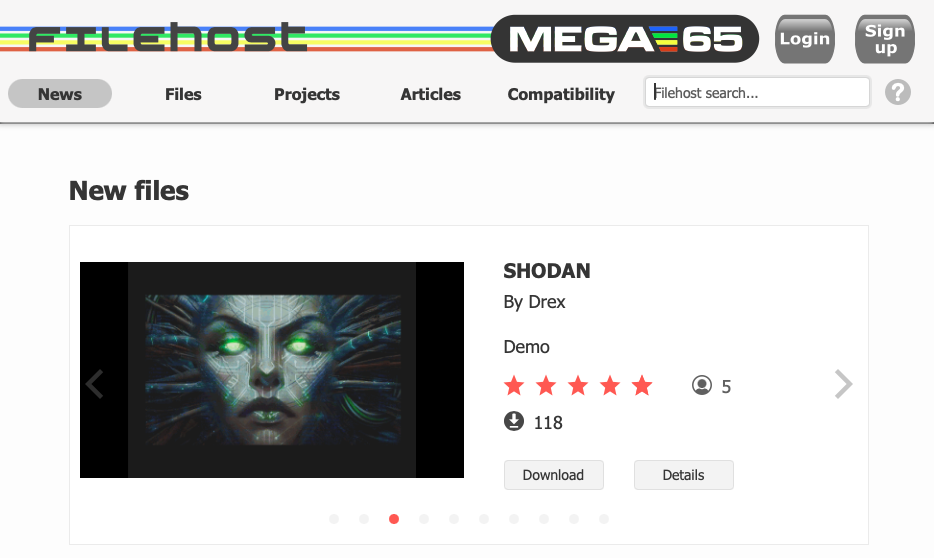
\includegraphics[width=0.7\linewidth]{images/filehost_notsignedin.png}}
\end{center}

Om een Filehost-account met uw eigenaarcode te registreren:

\begin{enumerate}
  \item Bezoek \href{https://files.mega65.org}{de Filehost-website}. Klik op ``Sign Up''. Volg de aanwijzingen om een account aan te maken.  \item Zoek uw eigenaarcode op.\index{Eigenaarscode} Dit is een code die op een papiertje staat afgedrukt; het papiertje was bij uw MEGA65 inbegrepen (mogelijk is het in deze handleiding gestoken). De code ziet er ongeveer als volgt uit: {\tt 123-ABC-456}  \item Klik in de rechterbovenhoek van het Filehost-scherm op het gebruikerspictogram. Selecteer in het pop-upmenu ``Redeem Code''. Voer uw eigenaarcode in zoals gevraagd.
\end{enumerate}

\begin{center}
  \fbox{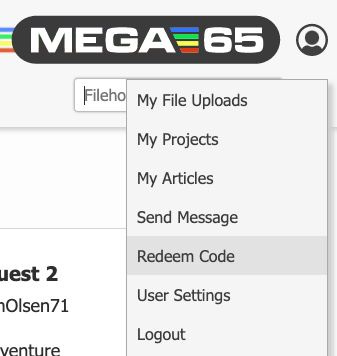
\includegraphics[width=0.4\linewidth]{images/filehost_redeemmenu.png}}
\end{center}

Om het nieuwste releasepakket te downloaden:

\begin{enumerate}
  \item Klik op het tabblad ``Files'' van de Filehost-website.  \item Typ in het zoekvak aan de linkerkant: ``core release''. De lijst wordt bijgewerkt en toont vervolgens alleen bestanden met deze woorden in de titel.  \item Zoek de vermelding genaamd ``MEGA65 Core Release Package (mega65r6) with ROM'', waarbij ``mega65r6'' overeenkomt met uw hardware-revisie. (Om uw hardware-revisie te bevestigen opent u het Freezer-menu en drukt u daarna op \specialkey{HELP}.)  \item Klik op de vermelding. Bevestig dat dit releasepakket voor uw hardware-revisie is en klik daarna op ``Download'' om het bestand te downloaden.
\end{enumerate}

\underline{OPMERKING}: Er bestaat een vermelding van het releasepakket zonder de ROM. Deze vermelding is voor iedereen zichtbaar. Om er zeker van te zijn dat u een compatibele set bestanden gebruikt, kiest u het pakket waarop ``with ROM'' staat. Indien u geen vermelding ziet waarop ``with ROM'' staat, controleer dan of u bent aangemeld en of u een geldige eigenaarcode heeft ingewisseld.

\begin{center}
  \fbox{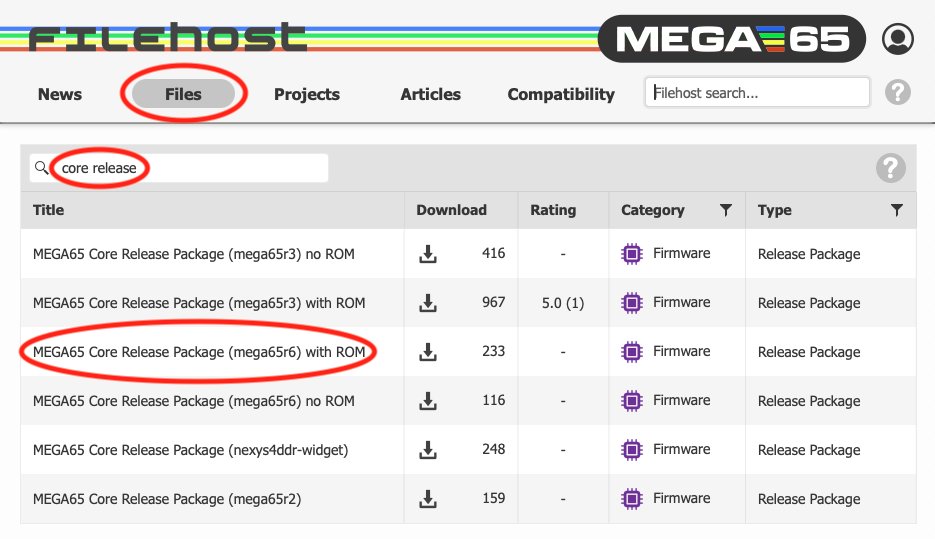
\includegraphics[width=0.7\linewidth]{images/filehost_release.png}}
\end{center}

Pak het gedownloade {\tt .7z}-archief uit. U zou een bestand moeten zien waarvan de naam eindigt op {\tt .cor} en een map {\tt sdcard-files} die een bestand bevat met de naam {\tt MEGA65.ROM}.

\section{Het corekeuzemenu}
\index{Core!Corekeuzemenu}

De MEGA65 bepaalt welke core bij het opstarten in de FPGA wordt geladen. U kunt dit proces onderbreken om te kiezen welke core wordt geladen.\footnote{Strikt genomen start de MEGA65 de core in slot 0 op om het corekeuzemenu te laten draaien. Nadat u een keuze hebt gemaakt of de computer een standaardcore kiest, laadt de computer de gekozen core in de FPGA en vervolgt hij het opstartproces.}

Om het corekeuzemenu te openen schakelt u de computer uit, houdt u de toets \specialkey{NO\\SCROLL} ingedrukt en schakelt u de computer weer in. Het corekeuzemenu verschijnt, met de acht coreslots, genummerd van 0 tot en met 7.

\begin{center}
  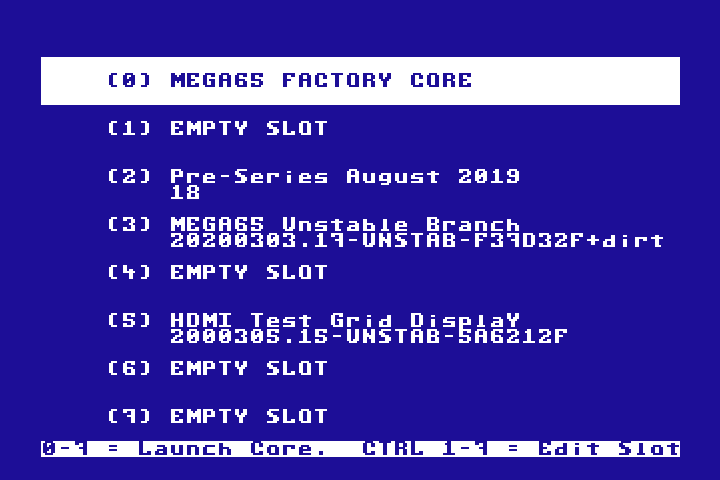
\includegraphics[width=0.7\linewidth]{images/ss-flashmenu.png}
\end{center}

U kunt met de cursortoetsen en \specialkey{RETURN} een core kiezen om op te starten, of u kunt eenvoudigweg de cijfertoets indrukken die overeenkomt met het slot. Het opstartproces wordt voortgezet met de nieuwe core. De MEGA65 blijft de nieuwe core gebruiken totdat u de computer uitschakelt. (Het indrukken van de resetknop wijzigt niet welke core wordt gebruikt.)

Wanneer u de computer inschakelt zonder het corekeuzemenu te openen, zoekt de MEGA65 naar een standaardcore. De computer controleert eerst of een core als standaardcore is gemarkeerd (een instelling die u kunt wijzigen). Indien geen enkele core zo is gemarkeerd, controleert de computer daarna of er een core in slot 1 staat.\footnote{Indien DIP-schakelaar \#4 in de stand ``on'' staat, controleert de MEGA65 slot 2 in plaats van slot 1. De DIP-schakelaars bevinden zich in de behuizing, op het moederbord.} Indien het slot leeg is, gebruikt de computer slot 0.

Uw computer is in de fabriek uitgerust met de MEGA65-core in slot 0. Wij raden u aan de in de fabriek geïnstalleerde core niet te upgraden, tenzij het MEGA65-team u dat adviseert. Installeer nieuwe versies van de MEGA65-core in plaats daarvan in slot 1.

\section{De core, ROM en systeembestanden upgraden}
\index{Core!Upgraden}\index{ROM!Upgraden}

Vanuit het corekeuzemenu kunt u een core upgraden of een nieuwe core installeren. Tijdens dit proces leest de computer het bestand {\tt .cor} van de SD-kaart.

Om de MEGA65-core, ROM en systeembestanden te upgraden:

\begin{enumerate}
  \item Verwijder de SD-kaart (of microSD-kaart) uit de MEGA65 en sluit deze met een SD-kaartlezer aan op uw PC.\footnote{In plaats van de SD-kaart naar uw PC over te brengen kunt u de bestanden ook via een Ethernet-verbinding overzetten. Zie hoofdstuk \vref{cha:transferring-files}.}  \item Kopieer het {\tt .cor}-bestand dat u uit het {\tt .7z}-archief hebt gehaald naar de SD-kaart.  \item Open op uw PC de map {\tt sdcard-files} uit het {\tt .7z}-archief en kopieer deze bestanden daarna naar de SD-kaart, waarbij u de bestaande bestanden vervangt. Plaats ze in de hoofdmap van het bestandssysteem van de SD-kaart, niet in een submap.  \item Werp de SD-kaart uit via het besturingssysteem van uw PC en plaats deze daarna terug in de MEGA65.  \item Open het corekeuzemenu: schakel de MEGA65 uit en houd daarna \specialkey{NO\\SCROLL} ingedrukt terwijl u de computer weer inschakelt.  \item Houd \specialkey{CTRL} ingedrukt en druk daarna op het cijfer van het slot dat u wilt upgraden. De sloteditor opent.  \item Druk op \megakey{F3} om een core-bestand te laden. De bestandsselectie opent. Gebruik de cursortoetsen om het {\tt .cor}-bestand te selecteren en druk daarna op \specialkey{RETURN}.  \item Druk op \megakey{F8} om het coreslot te flashen. Laat het flashen volledig verlopen. Dit duurt enkele minuten.  \item Wanneer het flashen is voltooid, drukt u op een willekeurige toets om terug te keren naar het corekeuzemenu.
\end{enumerate}

De sloteditor ziet er als volgt uit:

\begin{center}
  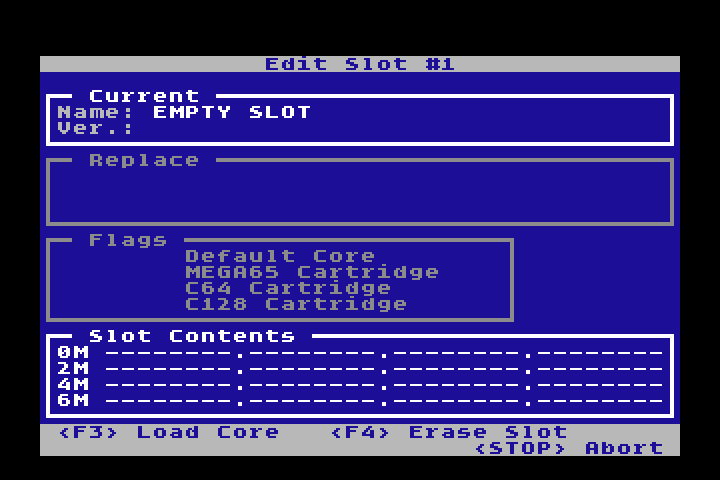
\includegraphics[width=0.7\linewidth]{images/ss-flashmenu-sloteditor.png}
\end{center}

Wanneer u een core-bestand laadt, vraagt de computer u het {\tt .cor}-bestand te selecteren op een scherm dat op dit voorbeeld lijkt:

\begin{center}
  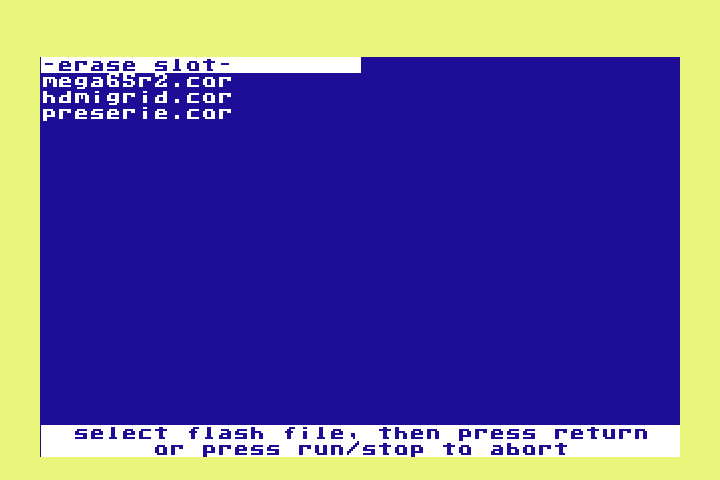
\includegraphics[width=0.7\linewidth]{images/ss-flashmenu-selectcore.png}
\end{center}

Nadat u de core hebt geselecteerd, toont de sloteditor welke wijziging deze in het slot wil aanbrengen. Wanneer u het flashen start, toont het beeldscherm de voortgang.

\underline{OPMERKING}: Schakel uw computer {\em niet} uit en onderbreek de stroomtoevoer niet voordat deze stap is voltooid.

\begin{center}
  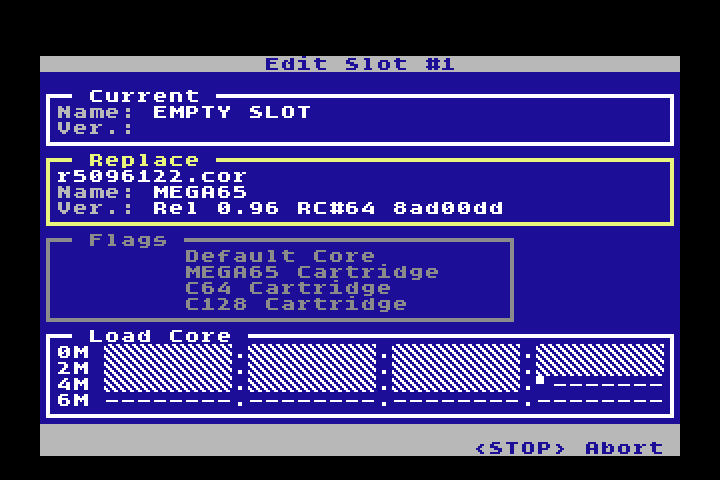
\includegraphics[width=0.7\linewidth]{images/ss-flashmenu-loading.png}
\end{center}

Wanneer de melding "Core was successfully flashed" wordt weergegeven, is het proces voltooid.

\begin{center}
  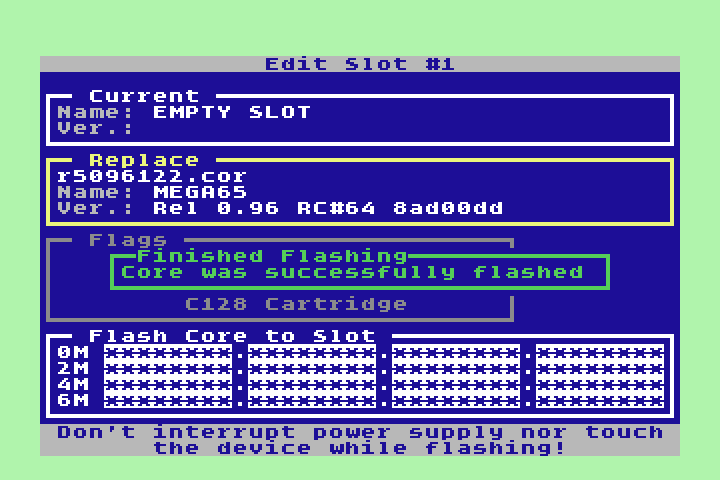
\includegraphics[width=0.7\linewidth]{images/ss-flashmenu-complete.png}
\end{center}

Het is nu veilig om uw computer uit te schakelen. Druk op een willekeurige toets om terug te keren naar het corekeuzemenu, of schakel de computer uit en daarna weer in om de standaardcore te starten.


\section{Alternatieve cores en ROM's installeren}

Het installeren van een alternatieve core, zoals de C64-core,\index{Core!C64-core} verloopt volgens dezelfde stappen voor het flashen van de core naar een slot.

Het is raadzaam de slots 2 tot en met 7 voor alternatieve cores te gebruiken en slot 1 voor de nieuwste MEGA65-core te reserveren. Er staat u uiteraard niets in de weg om een alternatieve core in slot 1 te installeren, zodat de MEGA65 zich bij het inschakelen als een ander type computer gedraagt. De MEGA65-core kunt u altijd kiezen via het corekeuzemenu.

U kunt meer dan één versie van de MEGA65-ROM op de SD-kaart bewaren. Wanneer u de MEGA65-core opstart, kunt u één van deze ROM's selecteren door tijdens het opstarten een cijfertoets ingedrukt te houden.

Om alternatieve ROM's te installeren kopieert u ze naar de hoofdmap van de SD-kaart, met een bestandsnaam zoals {\tt MEGA65x.ROM}, waarbij {\tt x} een getal tussen 0 en 8 is. Om de alternatieve ROM op te starten houdt u de bijbehorende cijfertoets ingedrukt terwijl de MEGA65-core start. Indien u geen cijfer ingedrukt houdt, start de computer standaard {\tt MEGA65.ROM} op.

Er zijn verschillende redenen waarom u alternatieve ROM's op uw SD-kaart zou willen bewaren:

\begin{itemize}
  \item U helpt een nieuwe bètaversie van de ROM te testen en u wilt de bètaversie niet tot uw standaard-ROM maken.
  \item U wilt de originele prototype-ROM van de Commodore 65 proberen. De MEGA65-core behoudt de achterwaartse compatibiliteit met de C65-ROM waaraan Commodore werkte voordat het bedrijf het project annuleerde. Deze ROM is gebrekkig en onvolledig, maar vormt nog steeds een interessant historisch artefact.
  \item U wilt een alternatieve ROM proberen die door de MEGA65-gemeenschap is ontwikkeld. Eén van deze ROM's is de MEGA65 OpenROM, een project om een volledig nieuwe ROM te maken die onder een open-sourcelicentie wordt uitgebracht, zonder enig oorspronkelijk Commodore-materiaal.
\end{itemize}

Bij uw MEGA65-SD-kaart werden diverse alternatieve ROM's meegeleverd, die in de fabriek zijn geïnstalleerd. Probeer uw computer opnieuw op te starten terwijl u een cijfertoets ingedrukt houdt en kijk wat er gebeurt!

\section{Core-vlaggen instellen}

Er zijn verschillende opties (``vlaggen'') die u voor een core in de core-editor kunt kiezen.

Om vlaggen voor een core te wijzigen bewerkt u het coreslot. Druk op de cijfertoets die overeenkomt met de vlag om de waarde ervan om te schakelen. Sla de vlaggen in het slot op door het resultaat te flashen: druk op \megakey{F8}. U kunt de vlaggen vóór het flashen van nieuwe coregegevens instellen, of u kunt alleen de nieuwe vlaginstellingen flashen zonder de coregegevens te vervangen.

Om een core in te stellen als de standaardcore, welke wordt gebruikt wanneer de MEGA65 wordt ingeschakeld zonder \specialkey{NO\\SCROLL} ingedrukt te houden, stelt u de vlag "Default core" in. Indien geen enkele core als standaardcore is ingesteld, wordt slot 1 als standaard gebruikt (of slot 2 indien DIP-schakelaar \#4 in de stand ``on'' staat).

De vlaggen "cartridge" bepalen welke core wordt geselecteerd wanneer er een cartridge in de expansiepoort aanwezig is. Zo kunt u op basis van het type cartridge een andere standaardcore kiezen. U kunt bijvoorbeeld de MEGA65-core instellen om MEGA65-cartridges af te handelen en een andere core om C64-cartridges af te handelen. Standaard handelt de MEGA65-core C64-cartridges af met behulp van de "GO64"-modus. Wellicht geeft u er de voorkeur aan dit te wijzigen en de C64-core te gebruiken die u afzonderlijk installeert.

\begin{center}
  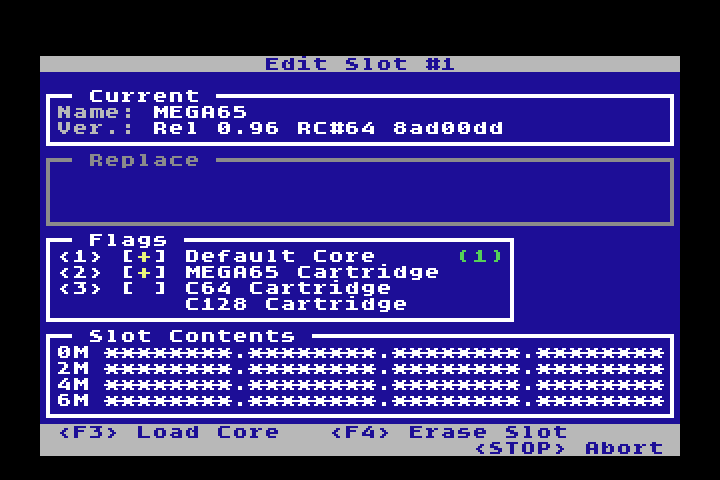
\includegraphics[width=0.7\linewidth]{images/ss-flashmenu-flags.png}
\end{center}

\section{Een coreslot wissen}

Het flashen vervangt wat er in een coreslot staat door de nieuwe core. Indien er al een core in het slot is geïnstalleerd, overschrijft het flashen de bestaande core.

Indien u een core wilt verwijderen en het slot leeg wilt laten, bewerkt u het slot en drukt u op \megakey{F4} om de vervanging in te stellen op "Erase slot". Druk daarna op \megakey{F8} om het slot met lege gegevens te flashen.

\section{De fabriekscore in slot 0 upgraden}
\index{Core!Fabriekscore in slot 0 upgraden}

Het is mogelijk de in de fabriek geïnstalleerde MEGA65-core in slot 0 te upgraden. Dit hoeft u alleen in zeldzame gevallen te doen, bijvoorbeeld indien een nieuwere versie van de MEGA65-core wijzigingen of foutcorrecties voor het opstartproces bevat. Het is raadzaam slot 0 niet te upgraden, tenzij de aankondiging van de uitgave daartoe aanleiding geeft. De meeste upgrades van de MEGA65-core zijn in slot 1 volledig functioneel, zonder dat u slot 0 hoeft te upgraden.

Het is belangrijk dat ten minste één coreslot een werkende MEGA65-core bevat. Indien er tijdens het flashen iets misgaat, kan dit leiden tot een niet-werkende core in dat slot. Om ongelukken te helpen voorkomen verschilt de procedure voor het flashen van slot 0 enigszins van die van de andere slots en kan alleen een officiële MEGA65-core naar slot 0 worden geflasht.

{\em Lees deze aanwijzingen zorgvuldig door voordat u met de procedure begint.} Om de core in slot 0 te upgraden:

\begin{enumerate}
  \item Installeer de nieuwste MEGA65-core in slot 1 met behulp van de hierboven beschreven procedure. De core moet zich in het standaardslot ongelijk aan nul bevinden om van eventuele problemen bij het upgraden van slot 0 te kunnen herstellen.  \item Start coreslot 1 op om te bevestigen dat het werkt.  \item Keer terug naar het corekeuzemenu: schakel de MEGA65 uit en houd daarna \specialkey{NO\\SCROLL} ingedrukt terwijl u de computer weer inschakelt.  \item Houd \megasymbolkey ingedrukt en druk op de komma-toets om de editor voor slot 0 te openen.  \item Lees het informatiescherm en typ daarna het woord {\tt CONFIRM} in hoofdletters en druk op \specialkey{RETURN}.  \item Herhaal de rest van de flashprocedure om het core-bestand te selecteren en het slot te flashen.
\end{enumerate}

\underline{OPMERKING}: Indien u een MEGA65 van revisie R3A heeft en slot 0 nog niet eerder heeft geüpgraded, starten \megasymbolkey en de komma-toets de procedure niet: u heeft een oudere core in slot 0 die deze voorziening niet heeft. U kunt dit omzeilen door het corekeuzemenu opnieuw te starten met slot 1. Bereid u vanuit het corekeuzemenu voor om \specialkey{NO\\SCROLL} ingedrukt te houden, druk op \megakey{1} om de core op te starten en druk daarna onmiddellijk op \specialkey{NO\\SCROLL} en houd deze ingedrukt. Het corekeuzemenu wordt daarna opnieuw geopend met behulp van slot 1. Druk op \megasymbolkey en de komma-toets om de upgrade van slot 0 te voltooien.

Indien er tijdens het flashen van slot 0 iets misgaat, start uw MEGA65 mogelijk niet correct op. Schakel uw MEGA65 vóór al het andere in en wacht ongeveer een minuut. Na enige tijd zou de computer moeten merken dat er geen geldige core in slot 0 staat en vervolgens de core in slot 1 starten. U kunt tijdens dit proces \specialkey{NO\\SCROLL} ingedrukt houden om het corekeuzemenu van slot 1 te openen en het flashen opnieuw te starten.

Indien de MEGA65 na enkele minuten nog geen enkele core kan opstarten, is de computer mogelijk vastgelopen. U kunt de computer wellicht herstellen met behulp van een apparaat dat een ``JTAG-interface'' heet en uw PC met het moederbord van de MEGA65 verbindt. Hiermee kunt u een bitstream rechtstreeks in de FPGA injecteren. Het onderdeel is goedkoop, doch niet altijd verkrijgbaar. Neem voor hulp contact op met het MEGA65-team via de Discord (\url{https://mega65.org/chat}).

Aan coreslot 0 kunnen geen vlaggen worden toegewezen, zoals een vlag om als standaardcore te dienen of om aan cartridgetypen te worden gekoppeld. Slot 0 wordt voor deze doeleinden gebruikt indien er geen andere core is geïnstalleerd. Het is raadzaam de nieuwste MEGA65-core in slot 1 te bewaren, naast het flashen van slot 0.


\section{Het opstartproces van de core begrijpen}
\nopagebreak
Deze sectie vat samen hoe de MEGA65 kiest met welke core hij bij het inschakelen opstart. Het proces wordt weergegeven in de volgende afbeelding:
\nopagebreak
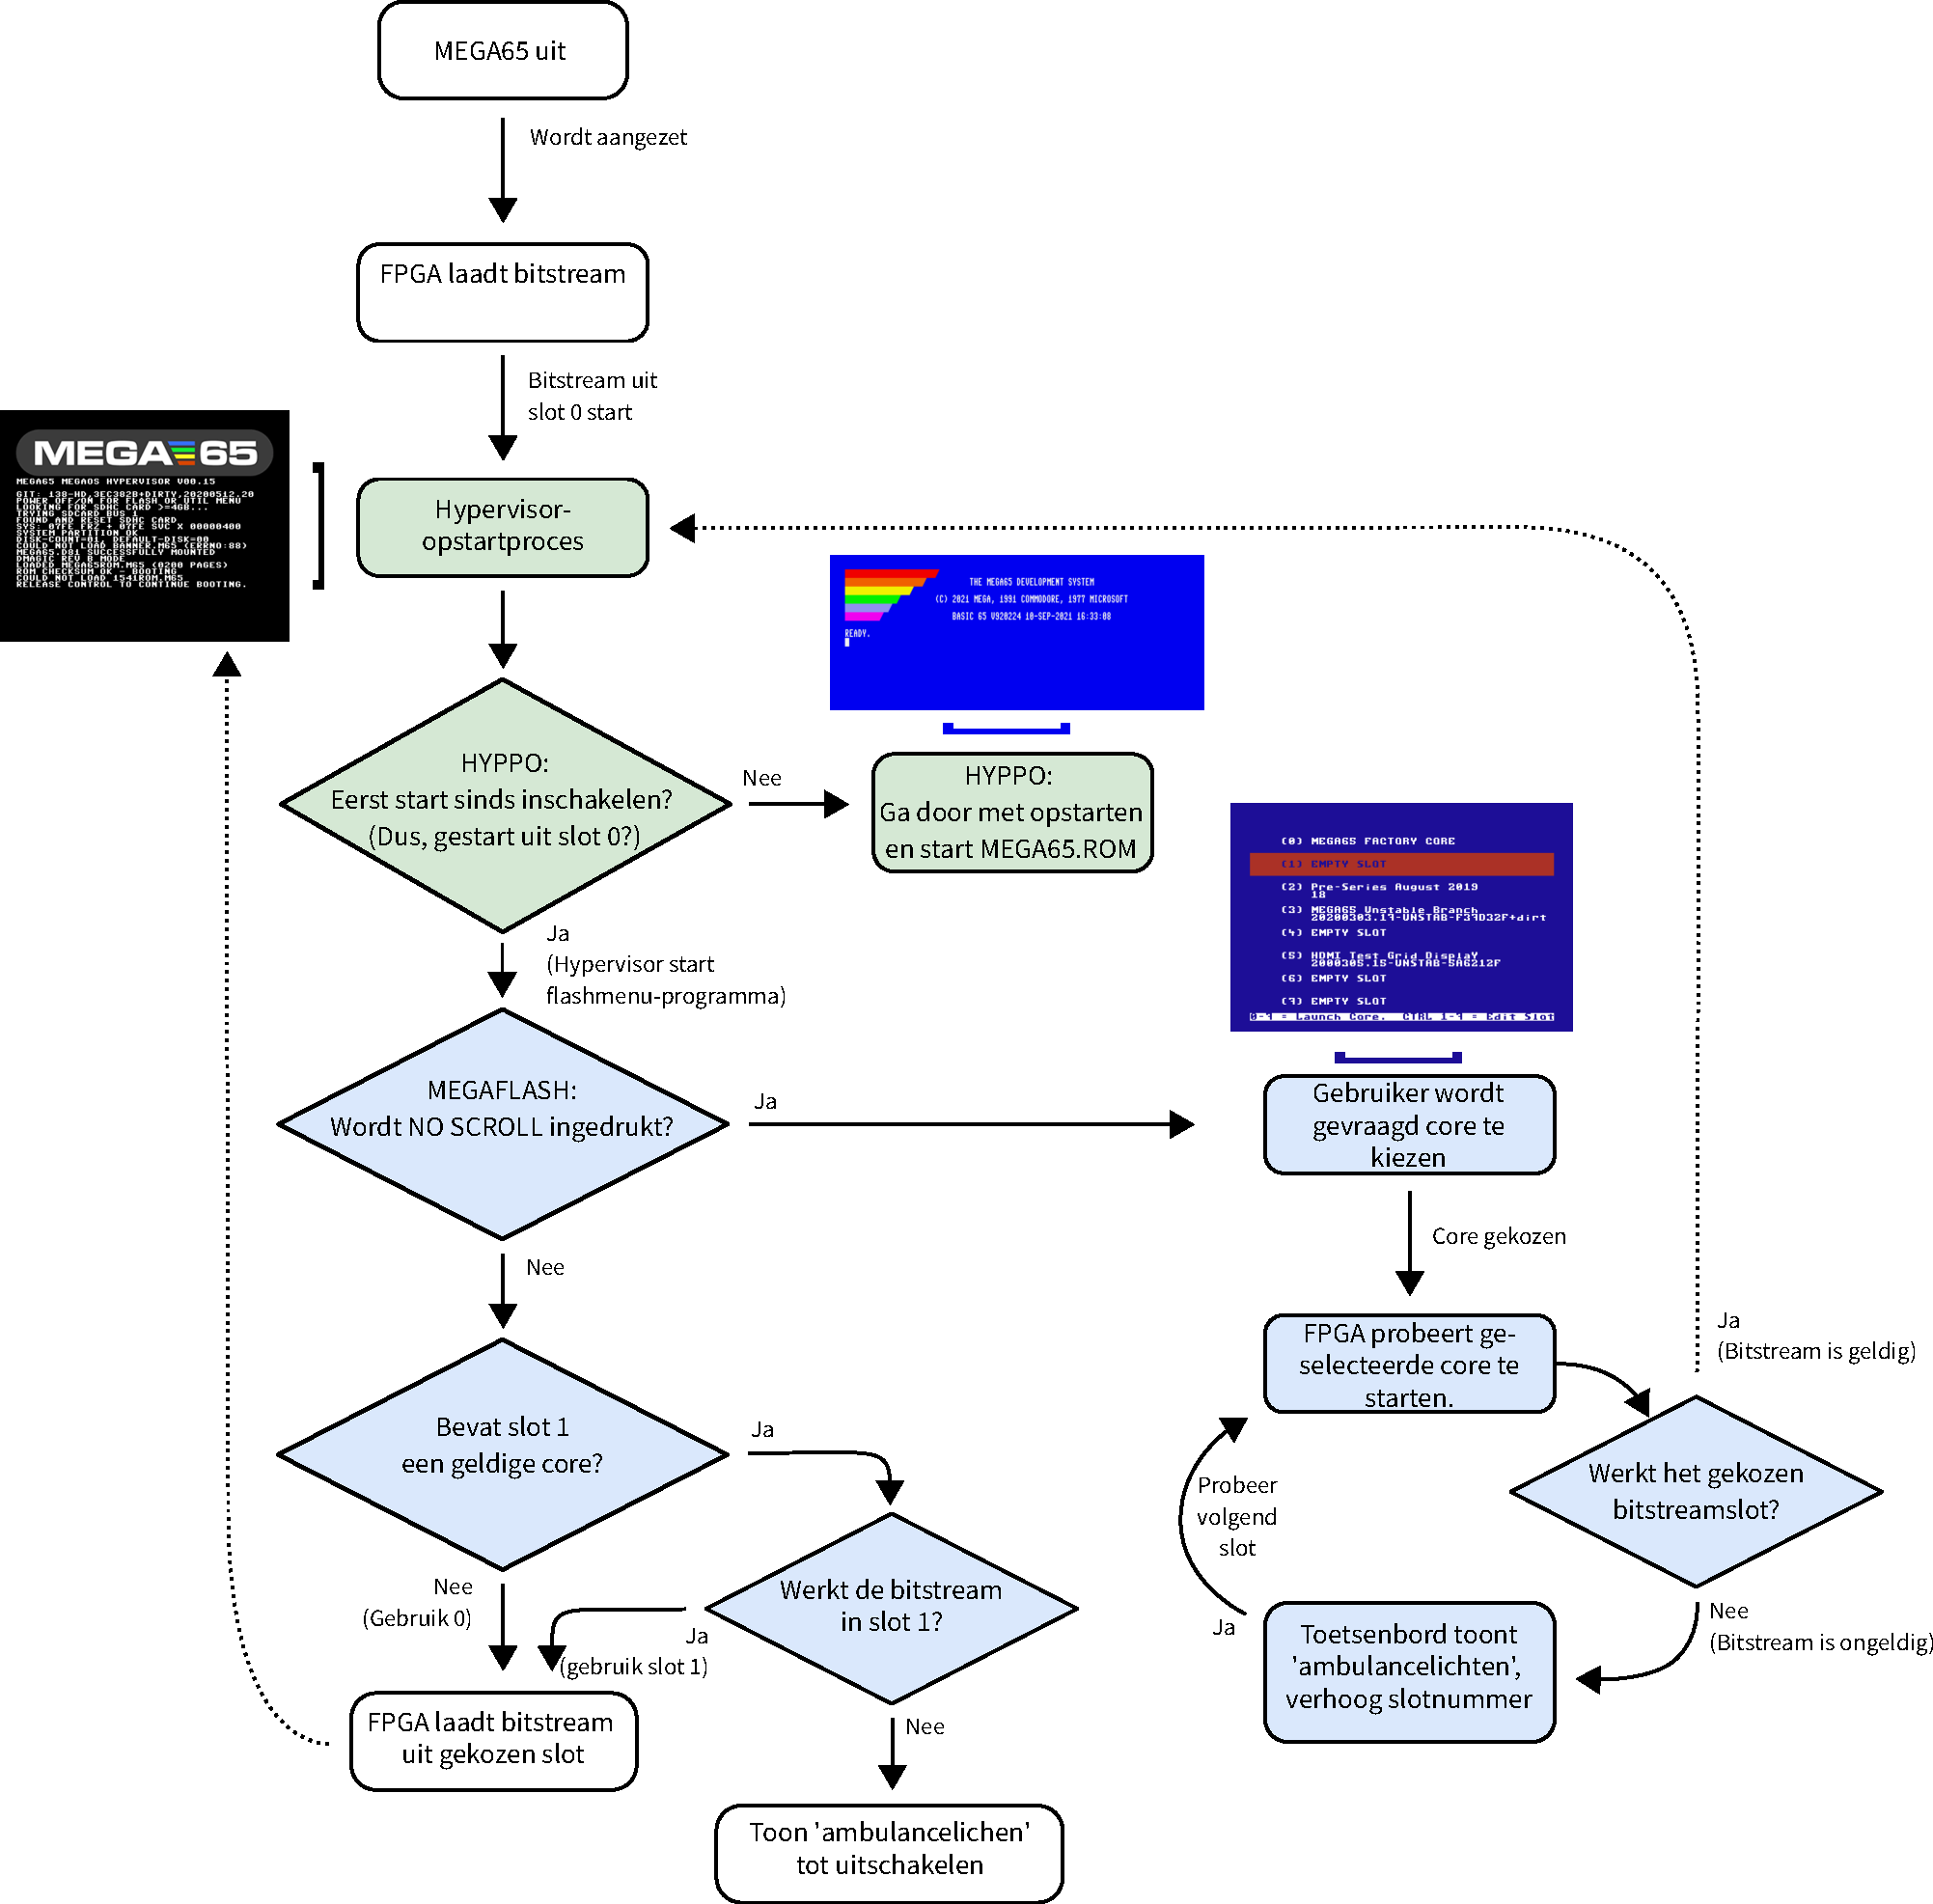
\includegraphics[width=\linewidth]{dutch/images/illustrations/flashmenu-flowchart.pdf}

Het opstartproces wordt beheerd door twee voorzieningen:
\begin{itemize}
  \item De Hypervisor (ook bekend als HYPPO), welke op een niveau boven de KERNAL werkt. Eén van zijn taken is het beheren van delen van het opstartproces. Raadpleeg voor meer details over de Hypervisor
\ifdefined\printmanual
{\bf Het grote Mega65-boek}.
\else
 \bookvref{sec:hypervisor-mode}.
\fi
    In het diagram zijn de activiteiten die de Hypervisor uitvoert groen gemarkeerd.  \item Het corekeuzemenuprogramma (ook bekend als ``MegaFlash''), welke een lijst met beschikbare coreslots biedt om uit te kiezen. In het diagram zijn de activiteiten die MegaFlash uitvoert blauw gemarkeerd.
\end{itemize}

Wanneer de MEGA65 wordt ingeschakeld, doet de computer het volgende:
\begin{itemize}
\item De MEGA65 laadt de bitstream in slot 0 van het flashgeheugen. Indien dat de MEGA65-fabriekscore is, start de HYPPO-hypervisor van de MEGA65.\item Indien het de eerste opstart na het inschakelen is (wat betekent dat u vanuit slot 0 werkt), start HYPPO het Flash-menu-programma (ook wel MegaFlash genoemd) -- maar houd er rekening mee dat het Flash-menu in deze modus mogelijk niets op het scherm toont om aan te geven dat het draait!\item Het Flash-menu controleert vervolgens of \specialkey{NO\\SCROLL} ingedrukt wordt gehouden.\item Indien dat het geval is, toont het Flash-menu zijn scherm, zodat u een core kunt selecteren of opnieuw flashen.\item Indien \specialkey{NO\\SCROLL} {\em niet} wordt ingedrukt gehouden, controleert het Flash-menu of Flash-slot 1 een geldige core bevat.\item Indien dat zo is, probeert het Flash-menu die core te laden.\item Indien dit lukt, herconfigureert het systeem zichzelf voor die core, waarna het gedrag van het systeem overeenkomt met die core.\item Indien dit mislukt, schakelt het toetsenbord over naar de ``ambulancemodus'', waarbij blauwe lampjes knipperen om aan te geven dat er eerste hulp nodig is. Merk op dat de resetknop in de ambulancemodus geen effect heeft: u moet de MEGA65 uitschakelen en weer inschakelen.
\end{itemize}

Indien u in het corekeuzemenu een andere core hebt geselecteerd, verloopt het proces op vergelijkbare wijze, met dit verschil dat de ambulancelampjes slechts gedurende een beperkte tijd branden: de FPGA zoekt namelijk automatisch door het flashgeheugen totdat hij een geldige core vindt. Indien hij het einde van het flashgeheugen bereikt, start hij de MEGA65-fabriekscore opnieuw vanuit slot 0.

\chapter{Werken met schijven en schijfimages}

\section{Schijfstations}
\label{cha:using-disks}
\index{Schijfstations}

De MEGA65 beschikt over een ingebouwd 3.5"-diskettestation en ondersteunt externe schijfstations in Commodore-stijl via de seriële IEC-poort aan de achterzijde van de computer. De IEC-poort ondersteunt ook andere externe IEC-opslagapparaten, zoals de SD2IEC.\index{SD2IEC-apparaat} Sommige IEC-opslagapparaten kunt u in een keten aansluiten en tegelijkertijd gebruiken.

De MEGA65 bevat ook een ``virtueel'' schijfstation dat D81- of D64-schijfimagebestanden\index{D81-schijfimage}\index{D64-schijfimage} op de SD-kaart kan aankoppelen. De meeste MEGA65-programmatuur die u van het internet downloadt, heeft de vorm van een D81-schijfimage. Programma's voor de Commodore 64 worden vaak verspreid in de vorm van een D64-schijfimage. U kunt rechtstreeks vanaf de MEGA65 een nieuw D81-schijfimage aanmaken en uw BASIC-programma's op de SD-kaart opslaan, zonder dat u extra hardware nodig hebt. U kunt ook bestanden kopiëren tussen fysieke floppy-schijven en schijfimages.

Het Intro Disk-menu\index{Intro Disk} dat u zag toen u de computer voor het eerst inschakelde, is een programma op een D81-schijfimage: een bestand met de naam {\tt MEGA65.D81} op de SD-kaart. De MEGA65 is in eerste instantie geconfigureerd om dit schijfimage automatisch op te starten. U kunt dit wijzigen in het Configuratiehulpprogramma.\index{Configuratie!Hulpprogramma} (Zie ook hoofdstuk \vref{cha:configuringyourmega}.)

U kunt schijfstations en virtuele schijfimages vanuit het Freezer-menu beheren.\index{Freezer-menu} Sommige van deze handelingen kunt u uitvoeren met BASIC-commando's zoals {\bf MOUNT}.\index{BASIC 65-commando's!MOUNT}

\subsection{Unitnummers en drivenummers}
\index{Schijfstations!Unitnummers en drivenummers}
\index{Aansluitingen!IEC}

Elk schijfstation (fysiek of virtueel) wordt benaderd via een {\it unit}nummer.\index{Unitnummer (IEC-apparaten)} Bij de vintage Commodore-computers verwijst het unitnummer naar een IEC-apparaat dat op de computer is aangesloten. Commodore reserveerde de unitnummers in het bereik 0 -- 31 voor apparaten met uiteenlopende doeleinden, waarvan 8 -- 11 voor schijfstations. Hebt u ooit een Commodore 64 gebruikt en \screentext{LOAD "*",8,1} ingetypt, dan verwijst de ``8'' naar het schijfstation dat als unit 8 is aangesloten. De schijfcommando's van BASIC 65 gebruiken standaard unit 8 en aanvaarden een {\bf U}-parameter om dit te wijzigen, bijvoorbeeld: \screentext{DLOAD "MYPROGRAM",U9}\index{BASIC 65-voorbeelden!DLOAD}\index{BASIC 65-voorbeelden!LOAD}

Bij de MEGA65 kunt u een unitnummer toewijzen aan het virtuele schijfstation met een gekoppeld schijfimage, of aan het ingebouwde 3.5"-diskettestation. U moet een schijfimage of het ingebouwde 3.5"-diskettestation aan een unitnummer koppelen voordat het gebruikt kan worden. Elk bericht dat naar een unitnummer wordt gestuurd dat aan een virtuele schijf of het ingebouwde diskettestation is toegewezen, wordt door de MEGA65 afgehandeld. Alle overige berichten worden naar de seriële IEC-poort gestuurd.

Schijfcommando's aanvaarden ook een optionele parameter om een {\it drive}nummer op te geven.\index{Drivenummer (IEC-apparaten)} Deze is alleen nodig bij het aansluiten van een vintage dubbel diskettestation via de IEC-poort, zoals de Commodore 4040, 8050 of 8250. Elk schijfstation kent drivenummer 0 toe aan het eerste station. Stations met twee schijven kennen drivenummer 1 toe aan het tweede station. Dubbele schijfstations zijn gewoonlijk uitgerust met een IEEE-488-interface en hebben een IEEE-488-naar-IEC-omzetter nodig om op de MEGA65 gebruikt te kunnen worden. De schijfcommando's van BASIC 65 gebruiken standaard drive 0 en aanvaarden een {\bf D}-parameter om dit te wijzigen.


\section{Werken met virtuele schijfimages}
\index{Schijfstations!Virtuele schijfimages}

De MEGA65 biedt twee ``beheerde stations'' die de via de IEC-poort aangesloten stations aanvullen. Aan het eerste beheerde station kunt u een D81- of D64-schijfimagebestand op de SD-kaart toewijzen, of u kunt het toewijzen aan het ingebouwde 3.5"-diskettestation. Aan het tweede beheerde station kunt u eveneens een D81- of D64-schijfimagebestand toewijzen, zodat er maximaal twee virtuele schijven tegelijkertijd gekoppeld kunnen worden.\footnote{Commodore was oorspronkelijk van plan een nieuw extern 3.5"-diskettestation uit te brengen, het ``1565''-station, dat bij de Commodore 65 zou horen en op een speciale niet-IEC-poort zou worden aangesloten. Het MEGA65-project heeft de ambitie om zo'n station ooit te produceren; indien dat gebeurt, zou dit station aan het tweede beheerde station worden toegewezen.}

Het eerste beheerde station kan worden ingesteld op unit 8 of 10 en het tweede beheerde station op unit 9 of 11.

\subsection{Waar u schijfimagebestanden kunt verkrijgen}

De website MEGA65 Filehost\index{Filehost-website} herbergt een bibliotheek met MEGA65-programmatuur die door de gemeenschap is gemaakt. U kunt door de programmatuur bladeren of erin zoeken, een titel downloaden en het schijfimage vervolgens met uw pc of met het Ethernet-bestandsoverdrachtshulpprogramma naar de SD-kaart kopiëren.

\url{https://files.mega65.org/}

\subsection{Schijfimages aankoppelen met de Freezer}

Open het Freezer-menu:\index{Freezer-menu} houd \widekey{RESTORE} één seconde ingedrukt en laat de toets vervolgens los. Let op de huidige toestand van aangekoppelde stations rechtsonder op het scherm.

\begin{center}
  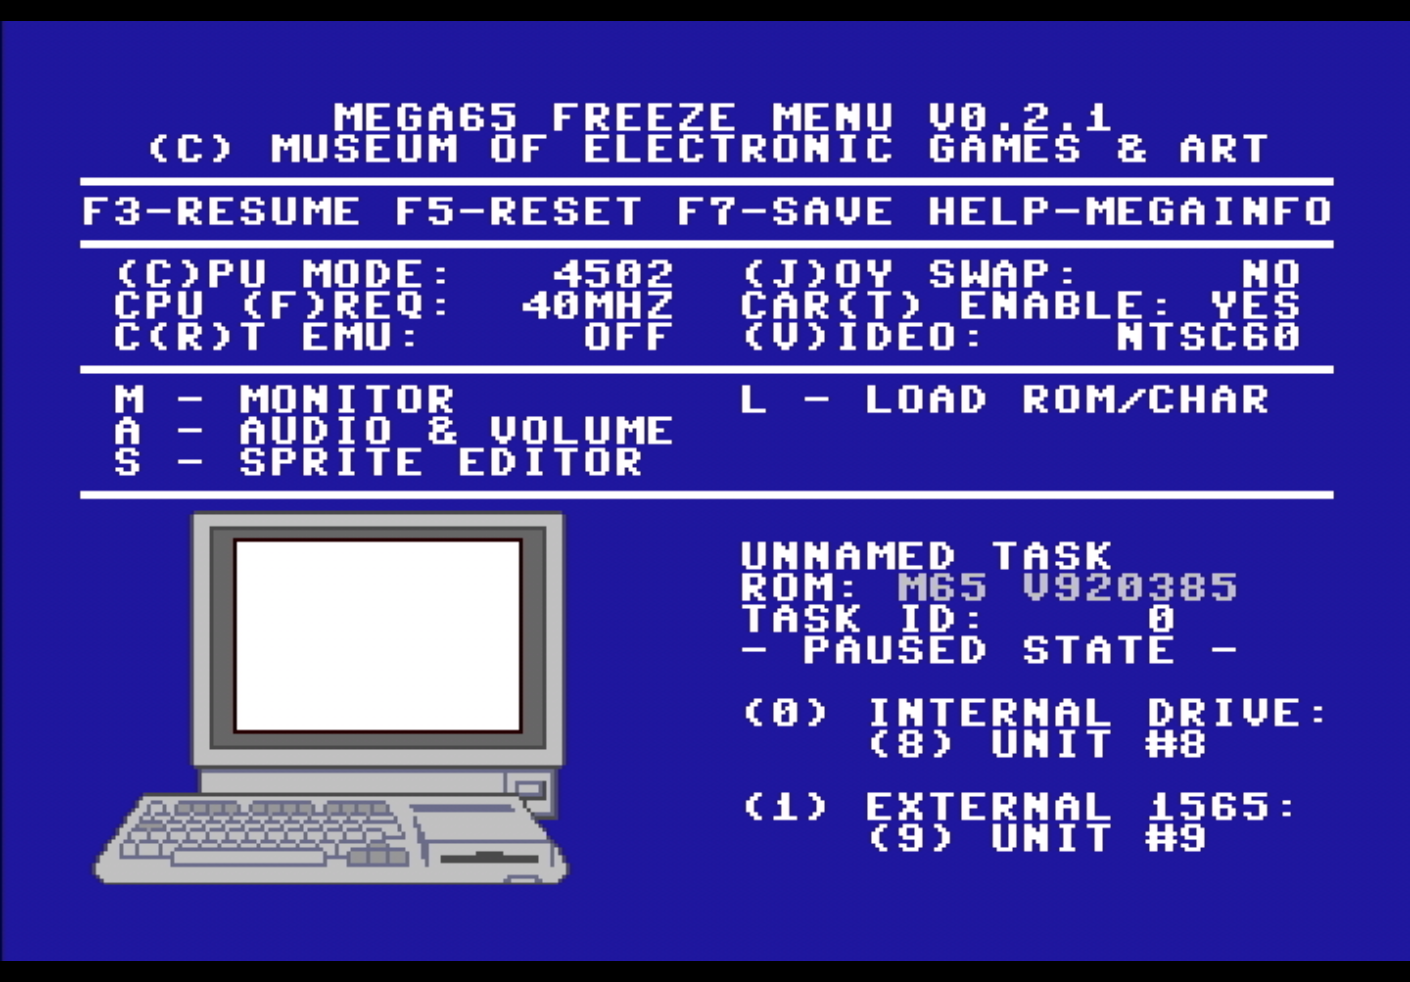
\includegraphics[width=0.7\linewidth]{images/freezer.png}
\end{center}

Om een schijfimage aan unit 8 of 10 te koppelen, selecteert u het eerste beheerde station door op \megakey{0} te drukken. Om een schijfimage aan unit 9 of 11 te koppelen, selecteert u het tweede beheerde station door op \megakey{1} te drukken. Dit opent de bestandsbrowser van de SD-kaart.

\begin{center}
  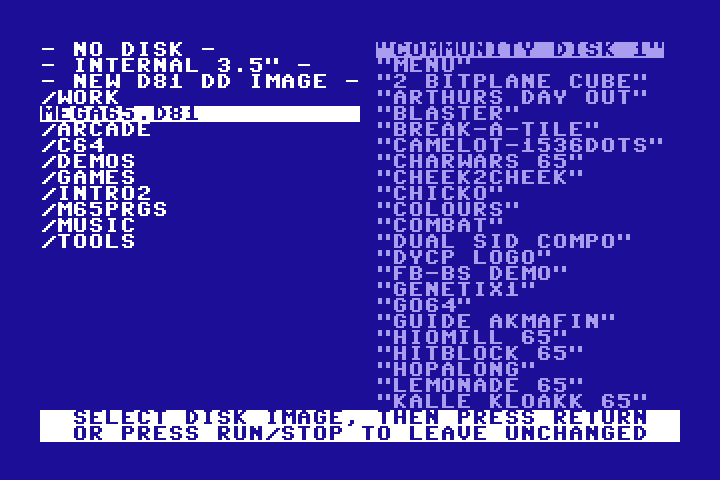
\includegraphics[width=0.7\linewidth]{images/d81-file-browser.png}
\end{center}

Gebruik de cursortoetsen om een schijfimage te selecteren en druk vervolgens op \widekey{RETURN}. Het Freezer-scherm toont dat het geselecteerde schijfimage nu aan het beheerde station is gekoppeld.

Druk vanaf het hoofdscherm van de Freezer op \megakey{8} of \megakey{9} om te wisselen tussen de unitnummers van respectievelijk het eerste en het tweede beheerde station.

\subsection{Schijfimages aankoppelen vanuit BASIC}

Met het BASIC-commando {\bf MOUNT}\index{BASIC 65-commando's!MOUNT} kunt u een schijfimage vanaf de SD-kaart aankoppelen zonder de Freezer te hoeven openen. U kunt dit commando bij de \screentext{READY}-prompt invoeren of het als onderdeel van een programma gebruiken.

Om een schijfimage aan unit 8 te koppelen, voert u {\bf MOUNT} in met de volledige bestandsnaam tussen dubbele aanhalingstekens, inclusief het achtervoegsel {\tt .D81} of {\tt .D64}:

\begin{screencode}
MOUNT "MEGA65.D81"
\end{screencode}

Om een schijfimage aan unit 9 te koppelen, geeft u het {\bf U}-argument op:

\begin{screencode}
MOUNT "MEGA65.D81",U9
\end{screencode}

\subsection{Een nieuw schijfimage aanmaken}
\index{Schijfstations!Virtuele schijfimages}

U kunt vanuit de Freezer van de MEGA65 een nieuw leeg D81-schijfimage aanmaken.\index{Freezer-menu}

\begin{enumerate}
\item Open de Freezer.\item Druk op \megakey{0} om het eerste beheerde station te selecteren.\item Selecteer boven in de bestandenlijst: \screentext{- NEW D81 DD IMAGE -}\item Voer, wanneer u daarom gevraagd wordt, een naam voor de schijf in. (Laat het achtervoegsel {\tt .D81} weg; dit wordt automatisch toegevoegd.)
\end{enumerate}

Het nieuwe schijfimage wordt op de SD-kaart aangemaakt en aan het eerste beheerde station gekoppeld. Het is geformatteerd en gereed voor gebruik.

\subsection{SD-kaartbestanden beheren in submappen}

Wanneer u enige tijd op Filehost games en toepassingen hebt gedownload, zult u uiteindelijk een grote verzameling schijfimages op uw SD-kaart hebben. Mogelijk wilt u deze bestanden in submappen ordenen. U kunt deze mappen aanmaken terwijl de SD-kaart op uw pc is aangesloten, of met het Ethernet-bestandsoverdrachtshulpprogramma.

De Freezer ondersteunt submappen in de bestandsbrowser. Elke submapnaam begint met een schuine streep (\screentext{/}). Selecteer een map om de bestanden ervan weer te geven. Om terug te keren naar de vorige map, selecteert u: \screentext{/..}

De MEGA65 houdt een ``huidige werkmap'' bij die als basismap dient voor BASIC-commando's zoals {\bf MOUNT}. Om de huidige werkmap vanuit BASIC te wijzigen, gebruikt u het {\bf CHDIR}-commando\index{BASIC 65-commando's!CHDIR} met het {\bf U12}-argument:\index{BASIC 65-voorbeelden!CHDIR}\index{BASIC 65-voorbeelden!MOUNT}

\begin{screencode}
CHDIR "DEMOS",U12

MOUNT "XANADU.D81"
\end{screencode}

\underline{OPMERKING}: De ondersteuning voor submappen op de SD-kaart is nog in ontwikkeling. Indien een schijfimage in een submap is gekoppeld, wordt het ontkoppeld door elke handeling die de huidige werkmap wijzigt. Sommige voorzieningen die bestanden gebruiken, ondersteunen mogelijk geen bestanden in submappen. Het is momenteel niet mogelijk om vanuit de Freezer een nieuw schijfimage in een submap aan te maken. Wij hopen dit in een toekomstige update te verbeteren.


\section{Het ingebouwde 3.5"-diskette\-station gebruiken}

De MEGA65 beschikt over een ingebouwd 3.5"-diskettestation, vergelijkbaar met wat voor de Commodore 65 bedoeld was. U kunt fysieke floppy-schijven gebruiken om uw programma's en gegevens op te slaan. Sommige MEGA65-programmatuur kan op diskette worden aangeschaft.

Het ingebouwde 3.5"-diskettestation moet gekoppeld worden voordat het gebruikt kan worden. Het kan aan unit 8 of unit 10 worden gekoppeld, in het eerste beheerde station.

\subsection{Het ingebouwde 3.5"-station aankoppelen met de Freezer}

Open het Freezer-menu:\index{Freezer-menu} houd \widekey{RESTORE} één seconde ingedrukt en laat de toets vervolgens los. Let op de huidige instellingen voor het aankoppelen van stations rechtsonder op het scherm.

Druk op \megakey{0} en gebruik vervolgens de pijltjestoets omlaag om \screentext{- INTERNAL 3.5" -} te selecteren. Druk op \widekey{RETURN} om de selectie te bevestigen. Het Freezer-menu toont dat het interne station aan het eerste beheerde schijfstation is gekoppeld.

Het \screentext{UNIT \#} voor het eerste station kan 8 of 10 zijn. Druk op \megakey{8} om tussen deze opties te wisselen. De schijfcommando's van BASIC 65 gebruiken standaard unit 8, dus het is gebruikelijk unit 8 te gebruiken tenzij u tegelijkertijd met meerdere schijven werkt.

Het ingebouwde 3.5"-diskettestation kan alleen in het eerste beheerde station worden gekoppeld, met unitnummers 8 of 10. Het kan niet in het tweede beheerde station worden gekoppeld (unitnummers 9 of 11).

\subsection{Het ingebouwde 3.5"-station aankoppelen vanuit BASIC}

U kunt het ingebouwde 3.5"-diskettestation met het BASIC-commando {\bf MOUNT} aan unit 8 koppelen. Dit commando werkt zowel vanaf de \screentext{READY}-prompt als vanuit een programma. Om het interne station aan unit 8 te koppelen, voert u het commando zonder argumenten in:\index{BASIC 65-voorbeelden!MOUNT}

\begin{screencode}
MOUNT
\end{screencode}

Het {\bf MOUNT}-commando kan het interne station alleen aan unit 8 koppelen. Vanuit het Freezer-menu kunt u het alleen aan unit 10 koppelen.

\subsection{DD- en HD-schijven}
\index{Schijfstations!Double-densityschijven (DD)}
\index{Schijfstations!High-densityschijven (HD)}

De schijfcontroller van de MEGA65 verwacht een diskette met Double Density (DD) in het ingebouwde 3.5"-diskettestation.\footnote{Het is mogelijk dat HD-schijven met volledige capaciteit in een toekomstige firmware-update worden ondersteund. De hardware van het station kan HD-schijven lezen.} Floppy-schijven worden niet meer geproduceerd en de DD-variant is tegenwoordig moeilijk te vinden.

U kunt een diskette met High Density (HD) in het station gebruiken, mits u één belangrijke wijziging aanbrengt: u moet beide zijden van het gat in de linkerbovenhoek (van voren gezien) van de schijf bedekken met een klein stukje plakband. Hierdoor laat u het station geloven dat de schijf DD is en schakelt het over naar een modus die compatibel is met de schijfcontroller van de MEGA65. Een DD-schijf heeft op deze plaats geen gat.

\begin{center}
  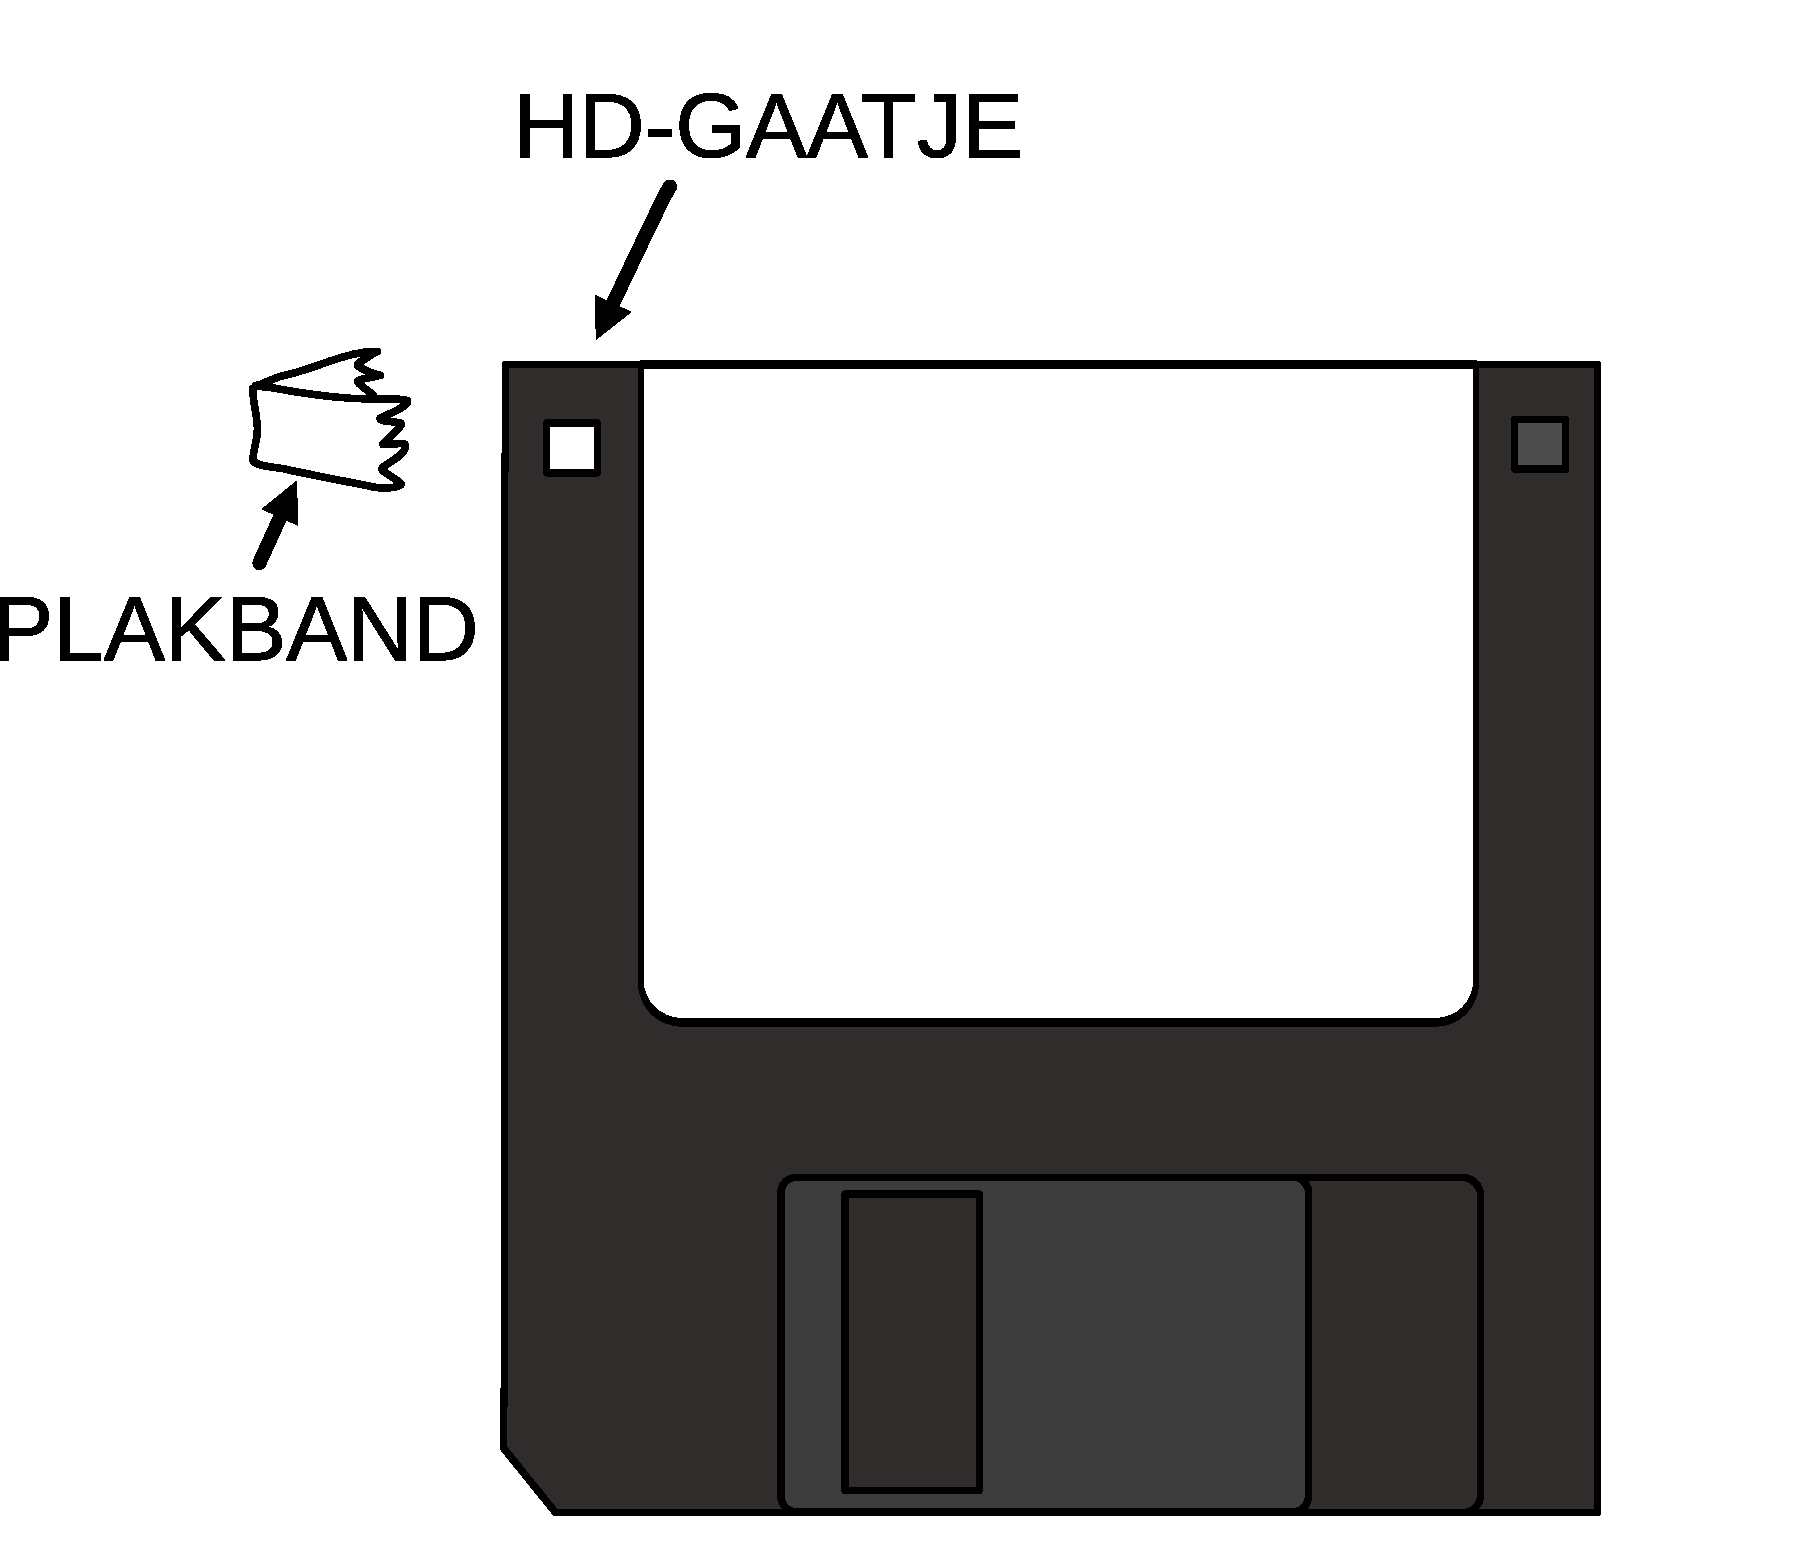
\includegraphics[width=0.75\textwidth]{dutch/images/illustrations/floppy_hd.pdf}
\end{center}

\underline{OPMERKING}: Zorg ervoor dat het plakband beide zijden van het gat bedekt.

\subsection{Een schijf formatteren}
\index{Schijfstations!Een schijf formatteren}

Een diskette moet geformatteerd worden voordat deze gebruikt kan worden. Het ingebouwde 3.5"-diskettestation van de MEGA65 emuleert een Commodore 1581-station en kan schijven gebruiken die in een dergelijk station zijn geformatteerd. U kunt een schijf ook met de MEGA65 formatteren.

\underline{OPMERKING}: Het formatteren van een schijf wist de inhoud ervan. Wees voorzichtig en doe dit uitsluitend wanneer u de gegevens op de schijf niet meer nodig hebt!

Voer de volgende stappen uit om een fysieke 3.5"-diskette met het interne station te formatteren:

\begin{enumerate}
\item Open het Freezer-menu.\index{Freezer-menu}\item Koppel het ingebouwde 3.5"-diskettestation aan het eerste beheerde station, unit 8.\item {\it Controleer dat unit 8 het volgende aangeeft:} \screentext{- INTERNAL 3.5" -}\item Hervat de computer: druk op \megakey{F3}.\item Plaats de diskette die u wilt formatteren in het interne diskettestation.\item Voer het BASIC-commando {\bf FORMAT} in en geef de schijf een naam ({\tt "MIJNDISK"}) en een ID van twee tekens ({\tt XX}).\index{BASIC 65-commando's!FORMAT}\index{BASIC 65-voorbeelden!FORMAT}
\begin{screencode}
FORMAT "MIJNDISK",IXX
\end{screencode}
\item Voer, wanneer u daarom gevraagd wordt, {\tt YES} in en druk op \widekey{RETURN}.
\end{enumerate}

Het formatteren van de schijf duurt ongeveer een minuut. Het station maakt tijdens het formatteren zoemende en klikkende geluiden. Schakel de computer niet uit en werp de schijf niet uit voordat het formatteren is voltooid.

U kunt bevestigen dat het formatteren is geslaagd door het {\bf DIR}-commando uit te voeren.\index{BASIC 65-commando's!DIR} U ziet dan een lege lijst van mappen met de naam en de ID die u hebt opgegeven. Uw schijf is nu gereed voor gebruik.


\section{Externe IEC-schijfstations gebruiken}
\index{Aansluitingen!IEC}

De MEGA65 werkt met externe schijfstations die op de seriële IEC-poort zijn aangesloten.

Externe stations hoeven niet te worden gekoppeld. Indien een unitnummer niet aan het ingebouwde 3.5"-diskettestation of aan een schijfimage is toegewezen, worden de schijfbewerkingen voor dat unitnummer naar de seriële IEC-poort verzonden. Het is aan het apparaat dat op de poort is aangesloten om zijn unitnummer te herkennen. Sommige IEC-apparaten hebben schakelaars waarmee u het unitnummer kunt instellen. Andere werken alleen met een specifiek nummer.

Indien u een extern station hebt dat een specifiek unitnummer verwacht, moet u ervoor zorgen dat de MEGA65 dat nummer niet aan een schijfimage of aan het interne station toewijst. Open het Freezer-menu\index{Freezer-menu} en druk vervolgens op \megakey{8} of \megakey{9} om de unitnummertoewijzingen om te schakelen, zodat zij het benodigde unitnummer niet meer gebruiken.\index{Unitnummer (IEC-apparaten)}

De station- en unitnummertoewijzingen zijn tijdelijk en worden teruggezet op hun standaardwaarden wanneer de MEGA65 wordt uitgeschakeld. U zult de stationtoewijzingen opnieuw moeten instellen wanneer u de computer de volgende keer inschakelt.


\section{Opstartbare schijven}
\index{Schijfstations!Opstartbare schijven}

Bij oudere Commodore-computers was het gebruikelijk dat softwaremakers de map op een diskette zo organiseerden dat het eerste bestand in de lijst het hoofdprogramma is. De gebruiker kon dan het commando \screentext{LOAD "*",8,1} invoeren om het hoofdprogramma te laden en \screentext{RUN} om het uit te voeren. Het sterretje is een jokerteken dat met elk bestand overeenkomt, dus ook met het eerste bestand op de schijf, zonder dat de gebruiker de naam van het programma hoeft te typen.

Deze methode is nog steeds gebruikelijk en de MEGA65 biedt een snelle manier om dergelijke schijven op te starten: houd \specialkey{SHIFT} ingedrukt en druk op \specialkey{RUN\\STOP}. Dit voert het commando \screentext{RUN "*"} uit, hetwelk vergelijkbaar is met de bekende commandoreeks die het eerste programma op de schijf laadt en uitvoert.\index{BASIC 65-commando's!RUN}

Met de C65 introduceerde Commodore een nieuwe manier om schijven op te starten. In plaats van te vertrouwen op de volgorde van bestanden, kan een schijf een bestand bevatten met de naam {\tt AUTOBOOT.C65}.\index{AUTOBOOT.C65-bestand} Indien dit bestand bestaat en een programma is, laadt en voert het BASIC-commando {\bf BOOT} dit bestand uit.\index{BASIC 65-commando's!BOOT}\index{BASIC 65-voorbeelden!BOOT}

\begin{screencode}
BOOT
\end{screencode}

\subsection{Schijven automatisch opstarten}

Zoals besproken in hoofdstuk \vref{cha:configuringyourmega}, kunt u het Configuratiehulpprogramma\index{Configuratie!Hulpprogramma} gebruiken om de MEGA65 in te stellen zodat hij tijdens het opstarten automatisch een virtueel schijfimage of het ingebouwde 3.5"-diskettestation koppelt.

Indien de gekoppelde schijf opstartbaar is --- dat wil zeggen dat hij een programmabestand met de naam {\tt AUTOBOOT.C65} bevat --- laadt en voert de MEGA65 het opstartprogramma automatisch uit.

Zo werkt de Intro Disk. Het Intro Disk-menu is een programma met de naam {\tt AUTOBOOT.C65} op het virtuele schijfimage {\tt MEGA65.D81}, hetwelk vooraf is ingesteld om bij het opstarten van het systeem gekoppeld te worden. Wanneer u de Intro Disk via het menu uitschakelt, hernoemt hij {\tt AUTOBOOT.C65} naar {\tt MENU}, zodat de schijf niet langer als opstartbaar wordt beschouwd.

Zelf een opstartschijf inrichten is een handige manier om uw computer te configureren. U kunt een kort BASIC-programma schrijven dat het systeemlettertype wijzigt, de achtergrondkleur aanpast en {\bf KEY}-macro's naar uw smaak instelt. Sla dit programma vervolgens op als {\tt AUTOBOOT.C65} op een schijf die u hebt geconfigureerd om bij het opstarten van het systeem aan te koppelen. Dit programma wordt elke keer uitgevoerd wanneer u uw MEGA65 inschakelt.


\section{De SD-kaart benaderen vanuit BASIC}

Verscheidene BASIC 65-commando's kunnen rechtstreeks op de SD-kaart van de MEGA65 werken alsof deze een schijfstation is. In deze gevallen staat de SD-kaart bekend als unit 12.

\underline{OPMERKING}: Unit 12 kan slechts voor enkele specifieke bewerkingen rechtstreeks worden benaderd. Hij kan de gehele SD-kaart niet als een CBDOS-schijf behandelen.

Om alle bestanden op de SD-kaart weer te geven, gebruikt u het {\bf DIR}-commando met het argument \screentext{U12}:\index{BASIC 65-commando's!DIR}\index{BASIC 65-voorbeelden!DIR}

\begin{screencode}
DIR U12
\end{screencode}

U kunt de optionele {\bf P}-vlag met dit commando gebruiken om de bestanden op de SD-kaart één pagina tegelijk weer te geven. Druk op Q om op de huidige pagina te stoppen, of op een willekeurige andere toets om naar de volgende pagina te gaan.

\begin{screencode}
DIR U12,P
\end{screencode}

Om een PRG-bestand rechtstreeks van de SD-kaart te laden (dat zich niet in een schijfimage bevindt), gebruikt u het \screentext{U12}-argument bij het {\bf DLOAD}-commando. In dit geval {\em moet} u het achtervoegsel {\tt .PRG} van de bestandsnaam opnemen, hetgeen verschilt van het gebruik van PRG-bestanden op schijven of in schijfimages. {\bf DSAVE} kan niet naar de SD-kaart opslaan met \screentext{U12} en meldt een fout als u het toch probeert; sla een programma daarom op in een schijfimage.\index{BASIC 65-commando's!DLOAD}\index{BASIC 65-commando's!DSAVE}\index{BASIC 65-voorbeelden!DLOAD}

\begin{screencode}
DLOAD "MIJNPROGJE.PRG",U12
\end{screencode}

Zoals eerder is besproken, ondersteunt de MEGA65 submappen op de SD-kaart en houdt een huidige werkmap bij voor schijfbewerkingen. Om de huidige werkmap te wijzigen naar een submap:\index{BASIC 65-commando's!CHDIR}\index{BASIC 65-voorbeelden!CHDIR}

\begin{screencode}
CHDIR "SUBDIR",U12
\end{screencode}

Om de huidige werkmap te wijzigen naar de bovenliggende map:

\begin{screencode}
CHDIR "..",U12
\end{screencode}

Het {\bf MOUNT}-commando kan een D81- of D64-schijfimage aan een unitnummer koppelen. Hoewel dit commando naar een bestand op de SD-kaart verwijst, maakt het geen gebruik van het \screentext{U12}-argument. In plaats daarvan stelt het commando met het {\bf U}-argument het unitnummer van de aan te koppelen schijf in. Het {\bf MOUNT}-commando gebruikt de door {\bf CHDIR} ingestelde huidige werkmap om het bestand te vinden.


\section{Gangbare schijfbewerkingen}

Hieronder vindt u enkele voorbeelden van gangbare schijfbewerkingen die u bij de \screentext{READY}-prompt kunt uitvoeren. Raadpleeg voor meer informatie de naslag over BASIC-commando's in bijlage \vref{cha:basic-reference}.

De meeste commando's die bestandsnamen aanvaarden, aanvaarden ook een {\bf U}-argument waarmee u aangeeft welke unit het bestand bevat. De standaardunit is 8.\footnote{Wanneer de computer voor het eerst wordt gestart, is de standaard schijfunit voor BASIC-commando's 8. U kunt deze wijzigen met het {\bf SET DEF}-commando.\index{BASIC 65-commando's!SET}}

\subsection{DIR}
\index{BASIC 65-commando's!DIR}\index{BASIC 65-voorbeelden!DIR}

Om de map (de lijst van bestanden) van een schijf weer te geven, gebruikt u het {\bf DIR}-commando.

\begin{screencode}
DIR

DIR U9
\end{screencode}

In tegenstelling tot de methode van de Commodore 64, waarbij de schijfmap in het BASIC-geheugen wordt geladen, wijzigt het {\bf DIR}-commando het BASIC-geheugen niet. U kunt {\bf DIR} veilig gebruiken wanneer er een programma in het geheugen staat.

Om grotere mappen gemakkelijker te kunnen bekijken, geeft {\bf DIR W} (van ``wide'') de map in kolommen weer en pauzeert na elke pagina.

\subsection{DLOAD en RUN}
\index{BASIC 65-commando's!DLOAD}\index{BASIC 65-voorbeelden!DLOAD}
\index{BASIC 65-commando's!RUN}\index{BASIC 65-voorbeelden!RUN}

Het {\bf DLOAD}-commando laadt een programma van de schijf in het geheugen. Het {\bf RUN}-commando voert het programma uit dat zich momenteel in het geheugen bevindt.

\begin{screencode}
DLOAD "GAAFSPEL"
RUN
\end{screencode}

U kunt beide tot één commando combineren door de bestandsnaam rechtstreeks aan het {\bf RUN}-commando te geven.

\begin{screencode}
RUN "GAAFSPEL"
\end{screencode}

\subsection{DSAVE}
\index{BASIC 65-commando's!DSAVE}\index{BASIC 65-voorbeelden!DSAVE}

Het {\bf DSAVE}-commando slaat het BASIC-programma dat zich momenteel in het geheugen bevindt op de schijf op.

\begin{screencode}
DSAVE "MIJNSPEL"
\end{screencode}

Standaard overschrijft dit geen bestaand bestand met dezelfde naam. Om een bestaand bestand te laten overschrijven, plaatst u een apestaartje vóór de bestandsnaam, binnen de dubbele aanhalingstekens.

\begin{screencode}
DSAVE "@MIJNSPEL"
\end{screencode}

Merk op dat opslaan met vervanging alleen wordt aanbevolen bij gebruik van schijfimages en het 3.5"-diskettestation. Oudere Commodore-stations bevatten fouten in deze functie die tot gegevensverlies kunnen leiden.

\subsection{BACKUP}
\index{BASIC 65-commando's!BACKUP}\index{BASIC 65-voorbeelden!BACKUP}

Het {\bf BACKUP}-commando kopieert een volledige schijf van de ene unit naar de andere. Hierbij worden alle bestaande gegevens op de bestemmingsschijf gewist.

\begin{screencode}
BACKUP U8 TO U9
\end{screencode}

U kunt {\bf BACKUP} gebruiken om schijfimages van floppy-schijven te maken, schijfimages naar floppy-schijven te schrijven of alles van het ene schijfstation naar het andere te kopiëren.

\subsection{COPY}
\index{BASIC 65-commando's!COPY}\index{BASIC 65-voorbeelden!COPY}

Het {\bf COPY}-commando maakt een kopie van een bestand. Indien bron en bestemming verschillende bestandsnamen op dezelfde unit zijn, dupliceert dit het bestand op de schijf. Wanneer u een bestand tussen units kopieert, behoudt het bestand zijn oorspronkelijke bestandsnaam. (Het nieuwe bestand kan met een afzonderlijk commando worden hernoemd.)

\begin{screencode}
COPY "MIJNSPEL", U8 TO U9

COPY "MIJNSPEL" TO "MIJNSPEL-V1"
\end{screencode}

\subsection{RENAME}
\index{BASIC 65-commando's!RENAME}\index{BASIC 65-voorbeelden!RENAME}

Het {\bf RENAME}-commando wijzigt de naam van een bestaand bestand.

\begin{screencode}
RENAME "MIJNSPEL-V29" TO "MIJNSPEL-GEREED"
\end{screencode}

\subsection{DELETE}
\index{BASIC 65-commando's!DELETE}\index{BASIC 65-voorbeelden!DELETE}

Het {\bf DELETE}-commando verwijdert een bestand.

\begin{screencode}
DELETE "ROMMELBESTAND"
\end{screencode}


\subsection{Snelkoppelingen voor schijfcommando's}

BASIC 65 biedt enkele snelkoppelingen voor gangbare schijfcommando's die u bij de \screentext{READY}-prompt kunt gebruiken.

\begin{center}
\begin{tabular}{|l|l|}
\hline
{\bf Snelkoppeling} & {\bf Overeenkomend commando} \\
\hline
\screentextwide{/} & {\bf LOAD} \\
\hline
$\uparrow$ & {\bf RUN} \\
\hline
$\leftarrow$ & {\bf SAVE} \\
\hline
\screentextwide{@} & {\bf DISK} \\
\hline
\screentextwide{\$} & {\bf DIR} \\
\hline
\end{tabular}
\end{center}

Deze snelkoppelingen zijn bedoeld om samen met een lijst van mappen programma's te starten zonder dat u bestandsnamen hoeft te typen. Bijvoorbeeld:

\begin{enumerate}
\item Geef de lijst van mappen van de schijf weer: typ {\bf \$} in en druk op \widekey{RETURN}.\item Gebruik de cursortoetsen om de cursor te verplaatsen naar de regel met het programma dat u wilt uitvoeren.\item Typ {\bf \screentext{$\uparrow$}} in en druk op \widekey{RETURN}.
\end{enumerate}

Het geselecteerde programma wordt geladen en uitgevoerd. Merk op dat u geen overtollige tekens van de regel hoeft te verwijderen. De snelkoppeling negeert alles behalve de bestandsnaam tussen dubbele aanhalingstekens, zoals die door de lijst van mappen wordt weergegeven.

\chapter{Bestanden overzetten}

\section{Bestanden naar de MEGA65 overbrengen}
\label{cha:transferring-files}
\index{SD-kaarten!Bestanden overzetten}

Het schrijven van uw eigen programma's voor de MEGA65 is erg leuk, maar uiteindelijk wilt u ook programma's uitvoeren die door anderen zijn geschreven. Wellicht wilt u ook een reservekopie van uw MEGA65-programma's op uw pc maken om ze veilig te bewaren.

De snelste en betrouwbaarste manier om bestanden tussen uw pc en uw MEGA65 over te zetten is met een Ethernet-kabel.\index{Netwerk!Ethernet} U sluit het ene uiteinde van de kabel aan op de RJ45-aansluiting aan de achterzijde van de MEGA65. U kunt het andere uiteinde aansluiten op de router of switch van uw local area network (LAN), of rechtstreeks op uw pc. U gebruikt software op uw pc om bestandsoverdrachten in beide richtingen te starten: van de pc naar de MEGA65 of van de MEGA65 naar de pc.

Als alternatief kunt u D81-virtuele schijfimages met behulp van een willekeurige pc met een SD-kaartlezer naar uw door de MEGA65 geformatteerde SD-kaart kopiëren, zonder andere speciale hulpmiddelen of software. Uw pc herkent het gegevensgebied van de SD-kaart als een FAT32-partitie. Indien u deze methode gebruikt, dient u zich ervan bewust te zijn dat sommige besturingssystemen van pc's ongewenste neveneffecten kunnen hebben, zoals fragmentatie van bestanden op de SD-kaart of overbodige bestanden die door macOS Finder worden aangemaakt. Deze effecten zijn onschadelijk voor de gegevens, maar kunnen onderhoud vergen om de kaart bruikbaar te houden in de MEGA65. Indien de MEGA65 meldt dat een bestand gefragmenteerd is, kunt u op de gegevenspartitie een defragmentatiehulpmiddel voor pc-schijven gebruiken. Als alternatief kunt u alle bestanden van de SD-kaart naar de pc kopiëren, de SD-kaart in de MEGA65 opnieuw formatteren en de bestanden vervolgens vanaf de pc terugkopiëren.

Het is ook mogelijk om bestanden over te zetten via een JTAG- of UART seriële interface die op het moederbord is aangesloten. Dit is een geavanceerde techniek en wordt niet in deze gebruikershandleiding beschreven. JTAG- of UART Serial-hardware biedt toegang tot een debuginterface die voor sommige programmeurs nuttig kan zijn. JTAG is ook nuttig voor het ontwikkelen van FPGA-cores. Zie voor meer informatie {\it De Mega65 programmeergids.}

De meeste mensen geven de voorkeur aan de Ethernet-methode. Dit hoofdstuk beschrijft hoe u dat doet.

\section{Netwerken begrijpen}

De MEGA65 kan Ethernet gebruiken om verbinding te maken met andere computers in een netwerk, of om verbindingen van andere computers te aanvaarden. Met de juiste programmatuur kan hij via het internet verbinding maken met andere computers.

De Ethernet-hardware van de MEGA65 biedt het lokale netwerk een Media Access Control (MAC)-adres aan.\index{Netwerk!MAC-adres} In tegenstelling tot andere Ethernet-hardware wordt het MAC-adres van de MEGA65 niet in de fabriek toegewezen: het wordt ingesteld in het configuratiehulpprogramma. (Zie hoofdstuk \vref{cha:configuringyourmega}.)

Om bestanden over te zetten, geeft u de MEGA65 opdracht zich beschikbaar te stellen voor binnenkomende verbindingen. Vervolgens gebruikt u op uw pc de M65Connect-app (of een ander hulpprogramma, zoals \texttt{mega65\_ftp}) om een verbinding tot stand te brengen. Het besturingssysteem van uw pc kan om toestemming vragen om het hulpprogramma toegang tot het netwerk te verlenen wanneer u het voor de eerste keer uitvoert. Het hulpmiddel gebruikt UDP-poort 4510 om de eerste verbinding met de MEGA65 tot stand te brengen en gebruikt voor de bestandsoverdrachtssessie een zelf toegewezen IPv6-adres dat op basis van het MAC-adres van de MEGA65 is aangemaakt. Hiervoor moet IPv6 op de netwerkinterface van de pc zijn ingeschakeld, wat in de meeste gevallen de standaardinstelling is.

Als alternatief voor de aansluiting op uw lokale netwerk kunt u de MEGA65, indien uw pc over een Ethernet-aansluiting beschikt, rechtstreeks met een Ethernet-kabel op uw pc aansluiten. Zo vormt u een klein lokaal netwerk zonder toegang tot het internet. De werkwijze voor het overzetten van bestanden is bij een rechtstreekse verbinding dezelfde als bij een verbinding via het lokale netwerk.

\section{M65Connect verkrijgen}
\index{M65Connect-toepassing}

{\bf M65Connect} is een toepassing voor Windows, Mac of Linux die bestandsoverdrachten en andere nuttige functies voor MEGA65-gebruikers mogelijk maakt. De toepassing beschikt over een interface met vensters en bevat tevens commandoregelhulpmiddelen die nuttig zijn bij het programmeren.

Om M65Connect te verkrijgen:

\begin{enumerate}
\item Bezoek de MEGA65 Filehost-website\index{Filehost-website} in een browser: \url{https://files.mega65.org}\item Typ in het zoekveld rechtsboven: ``M65Connect''\item Selecteer de versie van M65Connect voor het besturingssysteem van uw pc.\item Klik op de knop ``Download''.\item Gebruik uw pc om het gedownloade archiefbestand uit te pakken.
\end{enumerate}

\subsection{M65Connect voor Windows}

De Windows-versie van M65Connect staat in de map ``M65Connect'': {\bf M65Connect.exe}. Zoals bij de meeste openbronprogrammatuur het geval is, kan Microsoft Defender weigeren de programmatuur uit te voeren en een dialoogvenster weergeven. Indien dit gebeurt, klikt u op ``More info'' en vervolgens op de knop ``Run anyway'' die verschijnt.

De commandoregelhulpmiddelen staan in een submap met de naam ``M65Connect Resources'', zoals: {\tt M65Connect Resources\textbackslash{}mega65\_ftp.exe}

\subsection{M65Connect voor macOS}

De macOS-versie van M65Connect is een Mac-toepassingsbundel: {\bf M65Connect.app}. Zoals bij de meeste openbronprogrammatuur het geval is, beschouwt macOS het niet als door de ontwikkelaar ondertekend en zal macOS weigeren het uit te voeren. U moet het kenmerk ``quarantine'' verwijderen om de toepassing te kunnen uitvoeren.

In de meeste versies van macOS kunt u het quarantainekenmerk het eenvoudigst verwijderen met een Terminal-opdracht:

\begin{enumerate}
\item Verplaats de M65Connect-app naar uw map Applications.\item Open de Terminal-app, die bij macOS is inbegrepen. U vindt deze in de map Applications, in een submap met de naam Utilities.\item Voer deze opdracht in: {\tt xattr -cr /Applications/M65Connect.app}
\end{enumerate}

U kunt de M65Connect-app nu met een dubbelklik uitvoeren.

De commandoregelhulpmiddelen bevinden zich in de map van de toepassingsbundel, zoals: {\tt /Applications/M65Connect.app/Contents/Resources/mega65\_ftp.osx}

\subsection{M65Connect voor Linux}

De Linuxversie van M65Connect bevindt zich in de map ``M65Connect'': {\bf M65Connect}. Dubbelklik erop om het uit te voeren.

De commandoregelhulpmiddelen staan in een submap met de naam ``M65Connect Resources'', zoals: {\tt M65Connect Resources/mega65\_ftp}

\section{Netwerkluisteren inschakelen}
\index{Netwerk!Luistermodus}

Standaard negeert de MEGA65 alle pogingen van andere computers om er via het netwerk verbinding mee te maken. Programmatuur welke op de MEGA65 draait, kan luisteren naar netwerkverbindingen, doch de MEGA65 doet dit niet uit zichzelf.

Om bestanden met M65Connect over te zetten, dient u de MEGA65 te laten luisteren naar binnenkomende verbindingspogingen van M65Connect. Druk op \specialkey{SHIFT} + \megakey{\pounds} om een netwerkluistersessie in te schakelen. Het stroomlampje knippert afwisselend geel en groen wanneer netwerkluisteren actief is.

\begin{center}
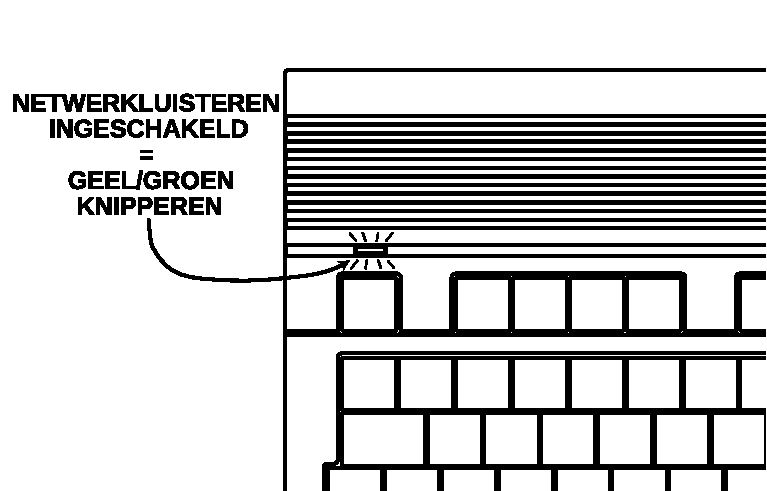
\includegraphics[width=\linewidth]{dutch/images/illustrations/mega65-eth-blink.pdf}
\end{center}

Druk opnieuw op \specialkey{SHIFT} + \megakey{\pounds} om netwerkluisteren uit te schakelen, of reset de computer.

Indien het stroomlampje na het indrukken van \specialkey{SHIFT} + \megakey{\pounds} niet begint te knipperen, moet u mogelijk DIP-schakelaar \#2 op het moederbord instellen. Bij MEGA65-modellen die in 2024 of later zijn gefabriceerd, hoort deze schakelaar in de fabriek ingesteld te zijn. Bij oudere MEGA65-modellen staat deze schakelaar standaard uit.

Om de DIP-schakelaar in te stellen,\index{DIP-schakelaars} opent u de behuizing zoals beschreven in hoofdstuk \vref{cha:setup}. Zoek de DIP-schakelaars op het moederbord en zet DIP-schakelaar \#2 in de positie ``on''. Zoek naar markeringen op de schakelaars om schakelaar \#2 en de richting ``on'' te herkennen. (De oriëntatie van uw DIP-schakelaars kan van dit diagram afwijken.)

\begin{center}
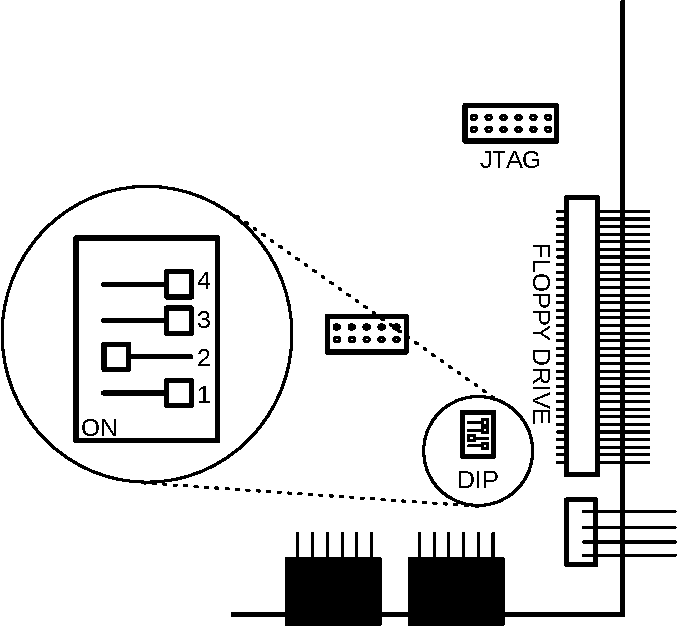
\includegraphics[width=\linewidth]{images/illustrations/mega65-dip2.pdf}
\end{center}

U kunt DIP \#2 gerust in deze positie laten staan voor normaal gebruik.


\section{Bestanden overzetten}

Om bestanden over te zetten, start u een bestandsoverdrachtssessie met de toepassing M65Connect of het commandoregelhulpmiddel {\tt mega65\_ftp}. Dit hulpmiddel maakt verbinding met de MEGA65 en uploadt een bestandsoverdrachtclient voor gebruik tijdens de sessie. Wanneer u de sessie beëindigt, reset de MEGA65.

Het starten van een bestandsoverdrachtssessie reset de MEGA65. Sla eventuele programma's of gegevens op voordat u verdergaat.

\underline{OPMERKING}: Indien u het geheugen wist door de computer te resetten, vergeet dan niet om netwerkluisteren opnieuw in te schakelen: druk op \specialkey{SHIFT} + \megakey{\pounds} en zorg dat het stroomlampje knippert.

\subsection{Bestanden overzetten met M65Connect}
\index{M65Connect-toepassing}

M65Connect detecteert automatisch of de MEGA65 naar verbindingen luistert. Open M65Connect en schakel vervolgens de netwerkluistersessie op de MEGA65 in. M65Connect meldt een status van "Connected to MEGA65 via LAN". M65Connect schakelt daarna in het venster diverse knoppen in, waaronder de {\bf PRG}- en {\bf SD Card}-knoppen.

\begin{center}
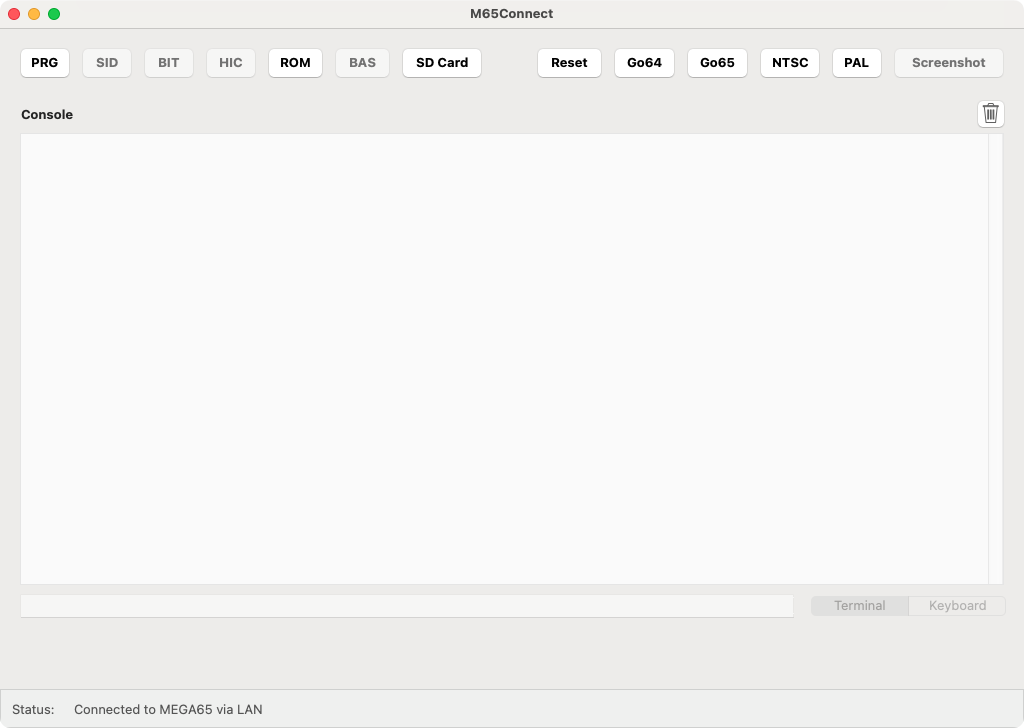
\includegraphics[width=\linewidth]{images/m65connect_macos.png}
\end{center}

Indien M65Connect een status van "Not connected to MEGA65" meldt, controleer dan het volgende:

\begin{itemize}
\item De MEGA65 en de pc zijn op hetzelfde netwerk aangesloten of rechtstreeks op elkaar via een netwerkkabel.\item De MEGA65 bevindt zich in de netwerkluistermodus met een knipperend stroomlampje.\item Open in M65Connect het menu Settings en selecteer Connections. Het veld "LAN Port" hoort een IPv6-adres te bevatten. Indien dat niet het geval is, wacht dan enkele seconden of klik op de knop "Autodetect LAN Port".
\end{itemize}

Klik op de knop {\bf SD Card} om een bestandsoverdrachtssessie te starten. Het SD Card Manager-venster gaat open.

\underline{OPMERKING}: Het starten van een bestandsoverdrachtssessie reset de MEGA65 om het bestandsoverdrachtshulpprogramma te laden. Zorg ervoor dat u eventuele gegevens op de MEGA65 hebt opgeslagen voordat u de sessie start.

\begin{center}
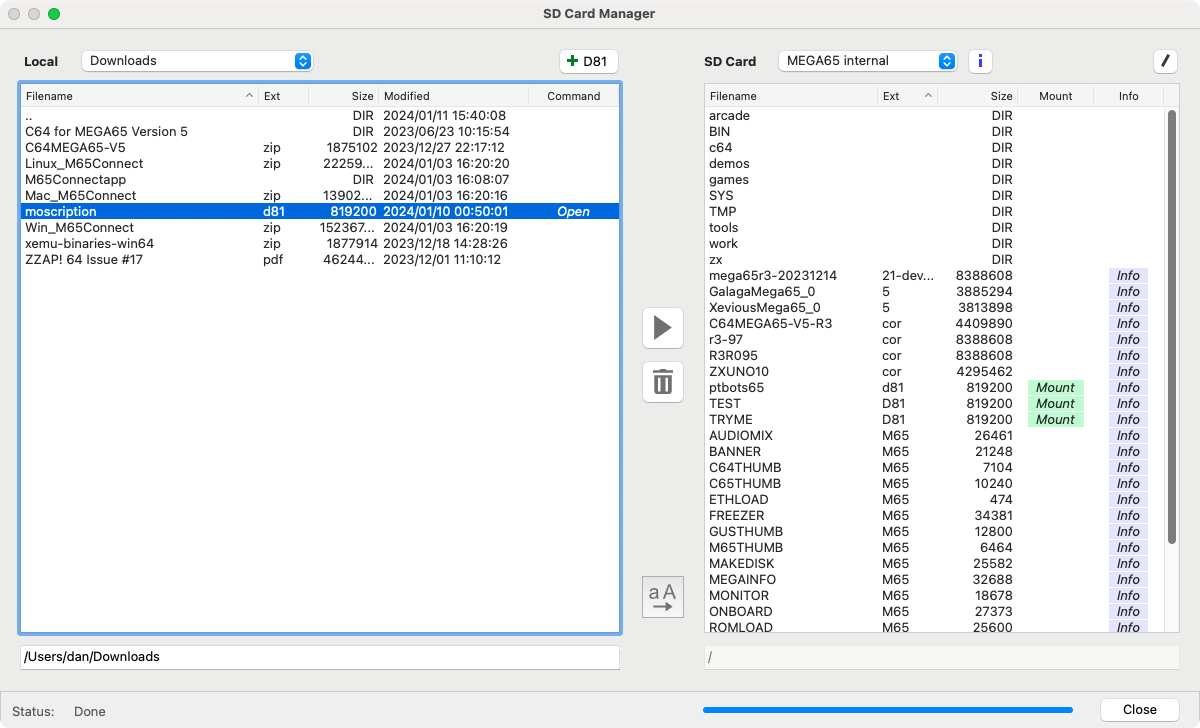
\includegraphics[width=\linewidth]{images/m65connect_files.png}
\end{center}

Gebruik het linkerdeelvenster om door de bestanden op uw pc te navigeren en het rechterdeelvenster om door de bestanden op de SD-kaart van de MEGA65 te navigeren. Selecteer het bestand en klik daarna op de pijlknop om het over te zetten. De knop geeft de richting aan waarin het bestand wordt overgezet.

U kunt M65Connect ook gebruiken om D81-schijfimages aan te maken en bestanden van en naar D81-schijfimages te kopiëren. Zoek een D81-schijfimage op uw pc of klik op de knop {\bf + D81} om er een aan te maken. Klik daarna in de bestandsverkenner op de opdracht "Open" om het schijfimage in het linkerdeelvenster te openen. Zet bestanden met de pijlknop over van en naar het schijfimage. Klik op de knop {\bf X} in de rechterbovenhoek om terug te keren naar de bestandsverkenner.

Klik op de knop {\bf Close} om de bestandsoverdrachtssessie te beëindigen en het SD Card Manager-venster te sluiten. Dit reset de MEGA65.

\subsection{Het commandoregelhulpmiddel mega65\_ftp}
\index{mega65\_ftp-commando@\texttt{mega65\_ftp-commando}}

Het commandoregelhulpmiddel {\tt mega65\_ftp} start een bestandsoverdrachtssessie met de MEGA65. Het kan interactief in de terminal draaien en meerdere bestandsoverdrachtopdrachten aanvaarden, of niet-interactief draaien met deze opdrachten als argumenten.

Om een interactieve bestandsoverdrachtssessie te starten, voert u de opdracht {\tt mega65\_ftp} uit en geeft u daarbij het argument {\tt -e} mee om aan te geven dat u een Ethernet-verbinding wilt gebruiken.

\underline{OPMERKING}: Het starten van een bestandsoverdrachtssessie reset de MEGA65 om het bestandsoverdrachtshulpprogramma te laden. Zorg ervoor dat u eventuele gegevens op de MEGA65 hebt opgeslagen voordat u de sessie start.

\begin{verbatim}
% mega65_ftp -e
\end{verbatim}

Het hulpprogramma uploadt de bestandsoverdrachtclient en u ziet de client op de MEGA65 draaien. Indien er niets gebeurt, drukt u op Ctrl-C (op de pc) om de overdracht af te breken en controleert u daarna nogmaals of de MEGA65 verbonden is en of netwerkluisteren is ingeschakeld.

Zodra de verbinding tot stand is gekomen, ziet de prompt voor bestandsoverdrachtopdrachten er ongeveer zo uit:

\begin{verbatim}
MEGA65 SD-Card:/>
\end{verbatim}

Om de sessie te beëindigen, gebruikt u de opdracht {\tt exit}. Het hulpprogramma sluit af, u keert terug naar de shellprompt en de MEGA65 reset.

\begin{verbatim}
MEGA65 SD-Card:/> exit
%
\end{verbatim}

Hieronder volgen enkele nuttige opdrachten die u tijdens de bestandsoverdrachtssessie kunt gebruiken. Gebruik de opdracht {\tt help} om een volledige lijst van de beschikbare opdrachten te zien.

\begin{center}
\begin{tabular}{|l|l|}
\hline
{\bf Opdracht} & {\bf Omschrijving} \\
\hline
{\tt put {\it bestandsnaam}} & Verstuurt een bestand van de pc naar de MEGA65. \\
\hline
{\tt get {\it bestandsnaam}} & Haalt een bestand op van de MEGA65 en plaatst het op de pc. \\
\hline
{\tt dir} & Toont een lijst van de mappen van de SD-kaart van de MEGA65. \\
\hline
{\tt ldir} & Toont een lijst van de huidige lokale werkmap. \\
\hline
{\tt mkdir {\it bestandsnaam}} & Maakt een submap aan op de SD-kaart van de MEGA65. \\
\hline
{\tt cd {\it bestandsnaam}} & Wijzigt de huidige werkmap op de SD-kaart van de MEGA65. \\
\hline
{\tt lcd {\it bestandsnaam}} & Wijzigt de huidige lokale werkmap. \\
\hline
{\tt help} & Toont een lijst met beschikbare opdrachten. \\
\hline
{\tt exit} & Beëindigt de bestandsoverdrachtssessie. \\
\hline
\end{tabular}
\end{center}

Om opdrachten van {\tt mega65\_ftp} aan te roepen zonder een interactieve prompt te starten, geeft u het argument {\tt -c} één keer per opdracht mee:

\begin{verbatim}
% mega65_ftp -e -c 'put mydisk.d81' -c 'exit'
\end{verbatim}

Het hulpprogramma start een sessie, voert de opdrachten uit en stopt vervolgens. Zorg ervoor dat u de opdracht {\tt exit} als laatste opdracht invoert om de MEGA65 te resetten, of reset de MEGA65 handmatig nadat de bestandsoverdracht is voltooid.

%% Use \appendix for compatibility with hyperref, but keep the "appendices"
%% environment for the "Appendices" entry in the table of contents.
\appendix
\begin{appendices}
  \def\drivedefinition{
{\bf station} stationnummer in dubbelschijfstations. Het stationnummer is standaard {\bf 0} en kan worden weggelaten bij enkelschijfstations zoals de 1541, 1571 of 1581.
}

\def\unitdefinition{
{\bf eenheid} apparaatnummer op de IEC-bus. Meestal van 8 t/m 11 voor schijfstations. Indien een variabele wordt gebruikt, moet deze tussen haakjes worden geplaatst. Het standaard eenheidsnummer is {\bf 8}.
}

\def\filenamedefinition{
{\bf bestandsnaam} de naam van een bestand. Ofwel een aangehaalde tekenreeks zoals \screentext{"DATA"}, of een tekenreeksexpressie in haakjes zoals: \screentext{(FI\$)}
}

\def\dirnamedefinition{
{\bf mapnaam} de naam van een map. Ofwel een aangehaalde tekenreeks zoals \screentext{"EENOFANDEREMAP"}, of een tekenreeksexpressie in haakjes zoals: \screentext{(DR\$)}
}

  \input{dutch/appendix-basic65-condensed}
  \chapter{PETSCII-codes}
\label{appendix:petsciicodes}

\section{PETSCII-codes}

PETSCII is de tekencodering die Commodore-8-bitcomputers gebruiken voor gegevens. De codering omvat afdrukbare tekens zoals letters, cijfers, leestekens en grafische symbolen; Controlcodes om de weergaveparameters te wijzigen en de cursor van de schermeditor te bedienen; en voorstellingen van toetsaanslagen die via het toetsenbord kunnen worden ingevoerd. Een programma kan PETSCII-codes gebruiken voor uitvoer naar het scherm, voor invoer via het toetsenbord of voor het lezen en schrijven van tekengegevens in bestanden of via seriële communicatie.

In BASIC aanvaardt de functie \textbf{CHR\$()} een PETSCII-code en geeft die code als string terug. Zo drukt \texttt{PRINT CHR\$(65)} de letter \screentext{A} af. De functie \textbf{ASC()} aanvaardt een string van één teken en geeft het getal van de PETSCII-code terug. De commando's \textbf{GET} en \textbf{GETKEY} lezen een toetsaanslag van het toetsenbord en geven de bijbehorende PETSCII-code terug.

Machinetaalprogramma's kunnen de GETIN-routine van de KERNAL of het PETSCIIKEY-hardwareregister gebruiken om toetsenbordinvoer als PETSCII-codes te lezen.

\index{Toetsenbord!PETSCII-codes en CHR\$}
\begin{adjustwidth}{}{-2cm}
\begin{multicols}{4}
\begin{description}[align=left,labelwidth=0.2cm]
    \item [0]    \item [1]   \small{Alternatief palet}    \item [2]   \small{Onderstrepen aan}    \item [3]    \item [4]   \small{Standaardpalet}    \item [5]   \small{Wit}    \item [6]    \item [7]   \small{Bel}    \item [8]    \item [9]   \specialkey{TAB}    \item [10]  \small{Nieuwe regel}
%   \item [11]  \footnotesize{DISABLE \specialkey{SHIFT}\megasymbolkey}
    \item [11]  Schakelt \\ \specialkey{SHIFT}\megasymbolkey uit
%   \item [12]  \footnotesize{ENABLE \specialkey{SHIFT}\megasymbolkey}
    \item [12]  Schakelt \\ \specialkey{SHIFT}\megasymbolkey in    \item [13]  \specialkey{RETURN}    \item [14]  \small{Kleine letters}    \item [15]  \small{Knipperen aan}    \item [16]  F9    \item [17]  \megakey{$\downarrow$}    \item [18]  \specialkey{RVS ON}    \item [19]  \specialkey{CLR\\HOME}    \item [20]  \specialkey{INST\\DEL}    \item [21]  F10 / Vorig woord    \item [22]  F11    \item [23]  F12 / Volgend woord    \item [24]  Tab instellen/wissen    \item [25]  F13    \item [26]  F14 / Vorig tabpunt    \item [27]  \small{ESCAPE}    \item [28]  \small{Rood}    \item [29]  \megakey{$\rightarrow$}    \item [30]  \small{Groen}    \item [31]  \small{Blauw}    \item [32]  \megakey{SPACE}    \item [33]  !    \item [34]  "    \item [35]  \#    \item [36]  \$    \item [37]  \%    \item [38]  \&    \item [39]  '    \item [40]  (    \item [41]  )    \item [42]  *    \item [43]  +    \item [44]  ,    \item [45]  -    \item [46]  .    \item [47]  /    \item [48]  0    \item [49]  1    \item [50]  2    \item [51]  3    \item [52]  4    \item [53]  5    \item [54]  6    \item [55]  7    \item [56]  8    \item [57]  9    \item [58]  :    \item [59]  ;    \item [60]  <    \item [61]  =    \item [62]  >    \item [63]  ?    \item [64]  @    \item [65]  A    \item [66]  B    \item [67]  C    \item [68]  D    \item [69]  E    \item [70]  F    \item [71]  G    \item [72]  H    \item [73]  I    \item [74]  J    \item [75]  K    \item [76]  L    \item [77]  M    \item [78]  N    \item [79]  O    \item [80]  P    \item [81]  Q    \item [82]  R    \item [83]  S    \item [84]  T    \item [85]  U    \item [86]  V    \item [87]  W    \item [88]  X    \item [89]  Y    \item [90]  Z    \item [91]  [    \item [92]  \pounds    \item [93]  ]    \item [94]  \megakeywhite{$\uparrow$}    \item [95]  \megakeywhite{$\leftarrow$}
\end{description}
\end{multicols}
\end{adjustwidth}

De codes 96 tot en met 127 drukken tekens af die vergelijkbaar zijn met die van de codes 192 tot en met 223. Zij worden niet als toetsenbordinvoer teruggegeven.

\begin{adjustwidth}{}{-2cm}
\begin{multicols}{4}
\begin{description}[align=left,labelwidth=0.2cm]
    \item [128]    \item [129] \small{Oranje}    \item [130] \small{Onderstrepen uit}    \item [131] \specialkey{SHIFT}\specialkey{RUN\\STOP}    \item [132] HELP    \item [133] F1    \item [134] F3    \item [135] F5    \item [136] F7    \item [137] F2    \item [138] F4    \item [139] F6    \item [140] F8    \item [141] \specialkey{SHIFT}\specialkey{RETURN}    \item [142] \small{Hoofdletters}    \item [143] \small{Knipperen uit}    \item [144] \small{Zwart}    \item [145] \megakey{$\uparrow$}    \item [146] \specialkey{RVS OFF}    \item [147] \specialkey{SHIFT}\specialkey{CLR\\HOME}    \item [148] \specialkey{SHIFT}\specialkey{INST\\DEL}    \item [149] \small{Bruin}    \item [150] \small{Lichtrood (roze)}    \item [151] \small{Donkergrijs}    \item [152] \small{Middengrijs}    \item [153] \small{Lichtgroen}    \item [154] \small{Lichtblauw}    \item [155] \small{Lichtgrijs}    \item [156] \small{Paars}    \item [157] \megakey{$\leftarrow$}    \item [158] \small{Geel}    \item [159] \small{Cyaan}    \item [160] \megakey{SPACE}    \item [161] \graphicsymbol{k}    \item [162] \graphicsymbol{i}    \item [163] \graphicsymbol{t}    \item [164] \graphicsymbol{[}    \item [165] \graphicsymbol{g}    \item [166] \graphicsymbol{<}    \item [167] \graphicsymbol{m}    \item [168] \graphicsymbol{/}    \item [169] \graphicsymbol{?}    \item [170] \graphicsymbol{m}    \item [171] \graphicsymbol{q}    \item [172] \graphicsymbol{d}    \item [173] \graphicsymbol{z}    \item [174] \graphicsymbol{s}    \item [175] \graphicsymbol{p}    \item [176] \graphicsymbol{a}    \item [177] \graphicsymbol{e}    \item [178] \graphicsymbol{r}    \item [179] \graphicsymbol{w}    \item [180] \graphicsymbol{h}    \item [181] \graphicsymbol{j}    \item [182] \graphicsymbol{l}    \item [183] \graphicsymbol{y}    \item [184] \graphicsymbol{u}    \item [185] \graphicsymbol{o}    \item [186] \graphicsymbol{\{}    \item [187] \graphicsymbol{f}    \item [188] \graphicsymbol{c}    \item [189] \graphicsymbol{x}    \item [190] \graphicsymbol{v}    \item [191] \graphicsymbol{b}    \item [192]  \graphicsymbol{C}    \item [193]  \graphicsymbol{A}    \item [194]  \graphicsymbol{B}    \item [195]  \graphicsymbol{C}    \item [196] \graphicsymbol{D}    \item [197] \graphicsymbol{E}    \item [198] \graphicsymbol{F}    \item [199] \graphicsymbol{G}    \item [200] \graphicsymbol{H}    \item [201] \graphicsymbol{I}    \item [202] \graphicsymbol{J}    \item [203] \graphicsymbol{K}    \item [204] \graphicsymbol{L}    \item [205] \graphicsymbol{M}    \item [206] \graphicsymbol{N}    \item [207] \graphicsymbol{O}    \item [208] \graphicsymbol{P}    \item [209] \graphicsymbol{Q}    \item [210] \graphicsymbol{R}    \item [211] \graphicsymbol{S}    \item [212] \graphicsymbol{T}    \item [213] \graphicsymbol{U}    \item [214] \graphicsymbol{V}    \item [215] \graphicsymbol{W}    \item [216] \graphicsymbol{X}    \item [217] \graphicsymbol{Y}    \item [218] \graphicsymbol{Z}    \item [219] \graphicsymbol{+}    \item [220] \graphicsymbol{-}    \item [221] \graphicsymbol{B}    \item [222] \graphicsymbol{\textbackslash}    \item [223] \graphicsymbol{]}

\end{description}
\end{multicols}
\end{adjustwidth}

De codes 224 tot en met 254 drukken tekens af die vergelijkbaar zijn met die van de codes 160 tot en met 190. Zij worden niet als toetsenbordinvoer teruggegeven.

De codes 126, 222 en 255 drukken alle drie het pi-symbool af (\graphicsymbol{\textbackslash}). Wanneer u dit teken typt, is de toetsenbordinvoercode 222.

Wanneer u de kleineletters-/hoofdlettermodus gebruikt (door \megasymbolkey + \specialkey{SHIFT} in te drukken), let dan op het volgende:
\begin{itemize}
  \item De hoofdletters in het gebied 65-90 van bovenstaande tabel worden vervangen door kleine letters.  \item De grafische tekens in het gebied 97-122 van bovenstaande tabel worden vervangen door hoofdletters.  \item De kleine letters van PETSCII (65-90) en de hoofdletters (97-122) vallen in het ASCII-gebied voor respectievelijk hoofdletters (65-90) en kleine letters (97-122).  \item Verscheidene symbolen hebben alternatieve symbolen in het lettertype voor kleine en hoofdletters, met name de PETSCII-codes 126, 127, 168 en 183.
\end{itemize}

  \chapter{Toetsen van de schermeditor}

\section{Toetsen van de schermeditor}

De volgende toetscombinaties voeren handelingen uit in de schermeditor van de MEGA65.

In sommige gevallen kan een programma de equivalente PETSCII-codes weergeven om dezelfde handelingen uit te voeren. Zo kan een programma \specialkey{CTRL} + \megakey{G}, welke een beltoon voortbrengt, als \screentext{CHR\$(7)} weergeven. Gebruik voor een \specialkey{ESC}-sequentie \screentext{CHR\$(27)} om de \specialkey{ESC}-toets weer te geven, gevolgd door de volgende toets van de reeks.

\section{Control-codes}
\label{appendix:controlcodes}
\index{Toetsenbord!CTRL}
\begin{center}
\setlength{\def\arraystretch{1.5}\tabcolsep}{6pt}
\begin{longtable}{c|L{5.5cm}}
	\textbf{Toetsencombinatie} & \textbf{Functie}\\
   \hhline{==}
	\endhead

  \multicolumn{2}{l}{\textbf{Kleuren}} \\
  \hhline{==}
\specialkey{CTRL} + \megakey{1} tot \megakey{8} &Kiezen uit het eerste kleurbereik. Zie bijlage \vref{appendix:colourtable} voor de lijst van kleuren in het systeempalet.\\
\hline
\megasymbolkey + \megakey{1} tot \megakey{8} &Kiezen uit het tweede kleurbereik.  \\
\hline
\specialkey{CTRL} + \megakey{E} &Herstelt de kleur van de cursor naar de standaardkleur (wit).\\
\hline
\specialkey{CTRL} + \megakey{D} &Schakelt de VIC-IV over naar kleurbereik 0-15 (standaardkleuren). Deze kleuren zijn bereikbaar met \specialkey{CTRL} en de toetsen \megakey{1} tot \megakey{8} (voor de eerste 8 kleuren) of met \megasymbolkey en de toetsen \megakey{1} tot \megakey{8} (voor de overige 8 kleuren).\\
\hline
\specialkey{CTRL} + \megakey{A} &Schakelt de VIC-IV over naar kleurbereik 16-31 (alternatieve/regenboog-kleuren). Deze kleuren zijn bereikbaar met \specialkey{CTRL} en de toetsen \megakey{1} tot \megakey{8} (voor de eerste 8 kleuren) of met \megasymbolkey en de toetsen \megakey{1} tot \megakey{8} (voor de overige 8 kleuren).\\
  \hhline{==}
  \multicolumn{2}{l}{\textbf{Tabposities}} \\
  \hhline{==}
\specialkey{CTRL} + \megakey{Z} &Verplaatst de cursor via een tab naar links. Indien er geen tabposities meer resteren, blijft de cursor aan het begin van de regel staan.\\
\hline
\specialkey{CTRL} + \megakey{I} &Verplaatst de cursor via een tab naar rechts. Indien er geen tabposities meer resteren, blijft de cursor aan het einde van de regel staan.\\
\hline
\specialkey{CTRL} + \megakey{X} &Stelt de huidige schermkolom als tabpositie in of wist deze.
 Gebruik \specialkey{CTRL} +\megakey{Z} en \megakey{I}  om heen en weer te springen naar alle posities die met \megakey{X} zijn ingesteld.\\
  \hhline{==}
  \multicolumn{2}{l}{\textbf{Verplaatsen}} \\
  \hhline{==}
\specialkey{CTRL} + \megakey{Q} &Verplaatst de cursor telkens één regel omlaag. Gelijk aan \megakey{$\downarrow$}.\\
\hline
\specialkey{CTRL} + \megakey{J} &Verplaatst de cursor één positie omlaag. Indien u zich op een lange regel BASIC-code bevindt die over twee regels doorloopt, verplaatst de cursor zich twee rijen omlaag om op de volgende regel te komen.\\
\hline
\specialkey{CTRL} + \megakey{]} &Gelijk aan \megakey{$\rightarrow$}.\\
\hline
\specialkey{CTRL} + \megakey{T} &Wist het teken direct links van de cursor en schuift alle tekens die rechts daarvan staan één positie naar links. Dit is gelijk aan \specialkey{INST\\DEL}.\\
\hline
\specialkey{CTRL} + \megakey{M} &Voert een regelterugloop uit, gelijk aan \specialkey{RETURN}.\\

  \hhline{==}
  \multicolumn{2}{l}{\textbf{Verplaatsen per woord}} \\
  \hhline{==}

\specialkey{CTRL} + \megakey{U} &Verplaatst de cursor terug naar het begin van het vorige woord. Indien er op de huidige regel geen vorig woord staat, verplaatst de cursor zich naar de eerste kolom van de huidige regel en vervolgens naar de vorige regel, totdat een regel met een woord wordt aangetroffen.\\
\hline
\specialkey{CTRL} + \megakey{W} &Verplaatst de cursor vooruit naar het begin van het volgende woord. Indien er op de huidige regel geen volgend woord staat, verplaatst de cursor zich naar de eerste kolom van de volgende regel, totdat een regel met een woord wordt aangetroffen.\\

  \hhline{==}
  \multicolumn{2}{l}{\textbf{Scrollen}} \\
  \hhline{==}

\specialkey{CTRL} + \megakey{P} &Schuift de BASIC-listing één regel omlaag. Gelijk aan \megakey{F9}.\\
\hline
\specialkey{CTRL} + \megakey{V} &Schuift de BASIC-listing één regel omhoog. Gelijk aan \megakey{F11}.\\
\hline
\specialkey{CTRL} + \megakey{S} &Gelijk aan \specialkey{NO\\SCROLL}.\\

  \hhline{==}
  \multicolumn{2}{l}{\textbf{Opmaak}} \\
  \hhline{==}

\specialkey{CTRL} + \megakey{B} &Schakelt de onderstrepingsmodus voor tekst in. U kunt de onderstrepingsmodus uitschakelen door \specialkey{ESC} en vervolgens \megakey{O} in te drukken.\\
\hline
\specialkey{CTRL} + \megakey{O} &Schakelt de flitsmodus voor tekst in. U kunt de flitsmodus uitschakelen door \specialkey{ESC} en vervolgens \megakey{O} in te drukken.\\
\hline

  \hhline{==}
  \multicolumn{2}{l}{\textbf{Hoofdlettergebruik}} \\
  \hhline{==}

\specialkey{CTRL} + \megakey{N} &Wijzigt het hoofdlettergebruik van de tekst van uitsluitend hoofdletters naar kleine letters.\\
\hline
\specialkey{CTRL} + \megakey{K} &Vergrendelt de omschakeling tussen hoofdletters en kleine letters, welke gewoonlijk met \megasymbolkey + \specialkey{SHIFT} wordt uitgevoerd.\\
\hline
\specialkey{CTRL} + \megakey{L} &Schakelt de omschakeling tussen hoofdletters en kleine letters in, welke met \megasymbolkey + \specialkey{SHIFT} wordt uitgevoerd.\\

  \hhline{==}
  \multicolumn{2}{l}{\textbf{Diversen}} \\
  \hhline{==}

\specialkey{CTRL} + \megakey{G} &Brengt een beltoon voort.\\
\hline
\specialkey{CTRL} + \megakey{[} &Gelijk aan het indrukken van \specialkey{ESC}.\\
\hline
\specialkey{CTRL} + \megakey{*} &Opent de Matrix Mode Debugger.\\
\hline

\end{longtable}
\end{center}


\section{Shiftcodes}
\label{appendix:shiftedcodes}
\index{Toetsenbord!Shifttoetsen}
\begin{center}
\setlength{\def\arraystretch{1.5}\tabcolsep}{6pt}
\begin{longtable}{c|L{5.5cm}}
	\textbf{Toetsencombinatie} & \textbf{Functie}\\
  \hhline{==}
	\endhead

\specialkey{SHIFT} + \specialkey{INST\\DEL} &Voegt op de huidige cursorpositie een teken in en verplaatst alle tekens één positie naar rechts.\\
\hline
\specialkey{SHIFT} + \specialkey{HOME} &Wist het volledige scherm en plaatst de cursor op de startpositie.\\
\hline

\end{longtable}
\end{center}



\section{Escape-sequenties}
\label{escape-sequences}
\index{Toetsenbord!Escape-reeksen}
Om een escape-sequentie uit te voeren, drukt u \specialkey{ESC} kort in en laat u deze weer los. Druk vervolgens één van de volgende toetsen in om de sequentie uit te voeren.

\begin{center}
\setlength{\def\arraystretch{1.5}\tabcolsep}{6pt}
\begin{longtable}{c|L{5.5cm}}
	\textbf{Toets} & \textbf{Sequentie}\\
  \hhline{==}
	\endhead

  \multicolumn{2}{l}{\textbf{Gedrag van de editor}} \\
  \hhline{==}

\specialkey{ESC} \megakey{X} &
Wist het scherm en schakelt tussen de tekstmodi 40 $\times$ 25 en 80 $\times$ 25.\\
\hline

\specialkey{ESC} \megakey{4} &
Wist het scherm en schakelt over naar de tekstmodus 40 $\times$ 25.\\
\hline

\specialkey{ESC} \megakey{8} &
Wist het scherm en schakelt over naar de tekstmodus 80 $\times$ 25.\\
\hline

\specialkey{ESC} \megakey{5} &
Schakelt over naar de tekstmodus 80 $\times$ 50.\\
\hline
\multicolumn{2}{L{7cm}}{  Let op dat sommige programma's verwachten dat zij in de tekstmodus 80 $\times$ 25 worden gestart en zich mogelijk niet correct gedragen wanneer zij in de tekstmodus 80 $\times$ 50 worden gestart.} \\
\hline

\specialkey{ESC} \megakey{@} &
%TODO the megakey with @ shows the label far smaller than any other key.
% Perhaps it needs more styling?
Wist een gedeelte van het scherm, vanaf de huidige cursorpositie tot het einde van het scherm.\\
\hline

\specialkey{ESC} \megakey{O} &
Schakelt de zinnebeeldmodus, de modus voor omgekeerde tekst, de onderstrepingsmodus en de flitsmodus uit.\\

  \hhline{==}
  \multicolumn{2}{l}{\textbf{Scrollen}} \\
  \hhline{==}
% TODO for some reason this doesn't leave enough space (the keys overlap with the hhline)
\specialkey{ESC} \megakey{V} &
Schuift het hele scherm één regel omhoog.\\
\hline
\specialkey{ESC} \megakey{W} &
Schuift het hele scherm één regel omlaag.\\
\hline
\specialkey{ESC} \megakey{L} &
Schakelt het scrollen in wanneer \megakey{$\downarrow$} onderaan het scherm wordt ingedrukt.\\
\hline
\specialkey{ESC} \megakey{M} &
Schakelt het scrollen uit. Wanneer \megakey{$\downarrow$} onderaan het scherm wordt ingedrukt, verplaatst de cursor zich naar de bovenkant van het scherm. Wanneer \megakey{$\uparrow$} echter bovenaan het scherm wordt ingedrukt, blijft de cursor op de eerste regel staan.\\
\hline
\specialkey{ESC} \megakey{N} &
Schakelt het ``regelduwen'' in: typen of afdrukken in de meest rechtse kolom schuift de daaropvolgende regels één positie omlaag.\\
\hline
\specialkey{ESC} \megakey{R} &
Schakelt het ``regelduwen'' uit: typen of afdrukken in de meest rechtse kolom verplaatst de cursor naar het begin van de volgende regel, maar schuift geen regels omlaag. Schakel zowel het ``regelduwen'' (\specialkey{ESC} \megakey{R}) als het scrollen (\specialkey{ESC} \megakey{M}) uit om met {\bf PRINT} in de meest rechtse kolom af te drukken zonder de rest van de weergave te verstoren.\\
\hhline{==}
  \multicolumn{2}{l}{\textbf{Invoegen en verwijderen}} \\
  \hhline{==}
\specialkey{ESC} \megakey{I} &
Voegt een lege regel in op de huidige cursorpositie en schuift alle daaropvolgende regels één positie omlaag.\\
\hline
\specialkey{ESC} \megakey{D} &
Verwijdert de huidige regel en schuift de regels onder de cursor één positie omhoog.\\
\hline
\specialkey{ESC} \megakey{P} &
Wist alle tekens van de cursor tot aan het begin van de huidige regel.\\
\hline
\specialkey{ESC} \megakey{Q} &
Wist alle tekens van de cursor tot aan het einde van de huidige regel.\\
  \hhline{==}
  \multicolumn{2}{l}{\textbf{Verplaatsen}} \\
  \hhline{==}
\specialkey{ESC} \megakey{J} &
Verplaatst de cursor naar het begin van de huidige regel.\\
\hline
\specialkey{ESC} \megakey{K} &
Verplaatst de cursor naar het laatste niet-witruimteteken op de huidige regel.\\
\hline
\specialkey{ESC} \megakeywhite{$\uparrow$} &
\index{Toetsenbord!Cursortoetsen}
Slaat de huidige cursorpositie op. Gebruik \specialkey{ESC} \megakeywhite{$\leftarrow$} (naast \megakey{1}) om de cursor terug te verplaatsen naar de opgeslagen positie. Let op: de \megakeywhite{$\uparrow$} die hier gebruikt wordt, staat naast \widekey{RESTORE}.\\
\hline
\specialkey{ESC} \megakeywhite{$\leftarrow$} &
Herstelt de cursorpositie naar de positie die eerder is opgeslagen door het indrukken van de toets \specialkey{ESC}
    \megakeywhite{$\uparrow$}
(naast \widekey{RESTORE}). Let op: de \megakeywhite{$\leftarrow$} die hier gebruikt wordt, staat naast \megakey{1}.\\
\hline
\specialkey{ESC} \specialkey{HOME} &
Herstelt de cursorpositie naar de positie die eerder is opgeslagen door het indrukken van \specialkey{HOME}.\\

  \hhline{==}
  \multicolumn{2}{l}{\textbf{Vensters}} \\
  \hhline{==}
\specialkey{ESC} \megakey{T} &
Stelt de linkerbovenhoek van het venstergebied in. Alle ingevoerde tekens en schermactiviteit blijven tot dit gebied beperkt. Zie ook \specialkey{ESC} \megakey{B}. U kunt de venstermodus uitschakelen door \specialkey{CLR\\HOME} tweemaal in te drukken. \\
\hline
\specialkey{ESC} \megakey{B} &
Stelt de rechterbenedenhoek van het venstergebied in. Alle ingevoerde tekens en schermactiviteit blijven tot dit gebied beperkt. Zie ook \specialkey{ESC} \megakey{T}. U kunt de venstermodus uitschakelen door \specialkey{CLR\\HOME} tweemaal in te drukken.\\
  \hhline{==}
  \multicolumn{2}{l}{\textbf{Gedrag van de cursor}} \\
  \hhline{==}
\specialkey{ESC} \megakey{A} &
Schakelt de automatische invoegmodus in. Elke ingedrukte toets wordt op de huidige cursorpositie ingevoegd, waarna alle tekens op de huidige regel rechts van de cursor één positie naar rechts opschuiven.\\
\hline
\specialkey{ESC} \megakey{C} &
Schakelt de automatische invoegmodus uit en keert terug naar de overschrijfmodus.\\
\hline
\specialkey{ESC} \megakey{E} &
Schakelt de cursor over naar de niet-flitsende modus.\\
\hline
\specialkey{ESC} \megakey{F} &
Schakelt de cursor over naar de gewone flitsmodus.\\
  \hhline{==}
  \multicolumn{2}{l}{\textbf{Gedrag van de bel}} \\
  \hhline{==}
\specialkey{ESC} \megakey{G} &
Schakelt de bel in. U kunt de bel laten klinken met \specialkey{CTRL} en \megakey{G}.\\
\hline
\specialkey{ESC} \megakey{H} &
Schakelt de bel uit, zodat het indrukken van \specialkey{CTRL} en \megakey{G} geen effect heeft.\\
  \hhline{==}
  \multicolumn{2}{l}{\textbf{Kleuren}} \\
  \hhline{==}
\specialkey{ESC} \megakey{U} &
\label{appendix:escape-colours}
Schakelt de VIC-IV over naar kleurbereik 0-15 (standaardkleuren). Deze kleuren zijn bereikbaar met \specialkey{CTRL} en de toetsen \megakey{1} tot \megakey{8} (voor de eerste 8 kleuren) of met \megasymbolkey en de toetsen \megakey{1} tot \megakey{8} (voor de overige kleuren).\\
\hline
\specialkey{ESC} \megakey{S} &
Schakelt de VIC-IV over naar kleurbereik 16-31 (alternatieve/rainbow-kleuren). Deze kleuren zijn bereikbaar met \specialkey{CTRL} en de toetsen \megakey{1} tot \megakey{8} (voor de eerste 8 kleuren) of met \megasymbolkey en de toetsen \megakey{1} tot \megakey{8} (voor de overige kleuren).\\
\hline
  \hhline{==}
  \multicolumn{2}{l}{\textbf{Tabposities}} \\
  \hhline{==}
\specialkey{ESC} \megakey{Y} &
Stelt de standaardtabposities in (om de 8 spaties) voor het volledige scherm.\\
\hline
\specialkey{ESC} \megakey{Z} &
Wist alle tabposities. Met \specialkey{CTRL} en \megakey{I} verplaatst een tab de cursor naar het einde van de regel.\\
\hline
\end{longtable}
\end{center}

  \chapter{Schermcodes}

\section{Schermcodes}

\label{appendix:screencodes}

Een tekstteken wordt in het schermgeheugen weergegeven door een schermcode. Er bestaan 256 mogelijke schermcodes, die elk verwijzen naar een afbeelding in de huidige tekenset.

Een volledige tekenset bevat twee groepen van 256 afbeeldingen: één voor de hoofdlettermodus en één voor de kleinelettermodus, derhalve 512 afbeeldingen in totaal. Slechts één modus kan tegelijk worden weergegeven. De ingebouwde tekensets gebruiken de eerste 128 tekens van elke groep voor normale tekens en de volgende 128 voor de geïnverteerde versies van dezelfde tekens.

In BASIC biedt de speciale array {\bf T@\&()} toegang tot de tekens op het scherm via kolom- en rij-indexen. De waarden in deze speciale array zijn schermcodes. Het {\bf FONT}-commando schakelt tussen de ingebouwde tekensets. Het {\bf CHARDEF}-commando wijzigt de afbeelding die bij een schermcode hoort.

\underline{OPMERKING}: Schermcodes verschillen van PETSCII-codes. PETSCII-codes worden gebruikt om tekstgegevens op te slaan, te verzenden en te ontvangen en om te bepalen hoe strings op het scherm worden weergegeven. Wanneer een PETSCII-teken op het scherm wordt weergegeven, wordt de bijbehorende schermcode in het schermgeheugen geschreven. Voor een overzicht van PETSCII-codes, zie bijlage \vref{appendix:petsciicodes}.

De volgende tabel geeft een overzicht van de schermcodes. Indien een code afhankelijk van de modus een ander teken oplevert, wordt het teken vermeld als ``hoofdletters / kleine letters''.

\index{Toetsenbord!Schermcodes}
\begin{adjustwidth}{}{-2cm}
\begin{multicols}{4}
\begin{description}[align=left,labelwidth=0.2cm]
    \item [0]   @    \item [1]   A / a    \item [2]   B / b    \item [3]   C / c    \item [4]   D / d    \item [5]   E / e    \item [6]   F / f    \item [7]   G / g    \item [8]   H / h    \item [9]   I / i    \item [10]  J / j    \item [11]  K / k    \item [12]  L / l    \item [13]  M / m    \item [14]  N / n    \item [15]  O / o    \item [16]  P / p    \item [17]  Q / q    \item [18]  R / r    \item [19]  S / s    \item [20]  T / t    \item [21]  U / u    \item [22]  V / v    \item [23]  W / w    \item [24]  X / x    \item [25]  Y / y    \item [26]  Z / z    \item [27]  [    \item [28]  \pounds    \item [29]  ]    \item [30]  $\uparrow$    \item [31]  $\leftarrow$    \item [32]  spatie    \item [33]  !    \item [34]  "    \item [35]  \#    \item [36]  \$    \item [37]  \%    \item [38]  \&    \item [39]  '    \item [40]  (    \item [41]  )    \item [42]  *    \item [43]  +    \item [44]  ,    \item [45]  -    \item [46]  .    \item [47]  /    \item [48]  0    \item [49]  1    \item [50]  2    \item [51]  3    \item [52]  4    \item [53]  5    \item [54]  6    \item [55]  7    \item [56]  8    \item [57]  9    \item [58]  :    \item [59]  ;    \item [60]  <    \item [61]  =    \item [62]  >    \item [63]  ?    \item [64]  \graphicsymbol{C}    \item [65]  \graphicsymbol{A} / A    \item [66]  \graphicsymbol{B} / B    \item [67]  \graphicsymbol{C} / C    \item [68]  \graphicsymbol{D} / D    \item [69]  \graphicsymbol{E} / E    \item [70]  \graphicsymbol{F} / F    \item [71]  \graphicsymbol{G} / G    \item [72]  \graphicsymbol{H} / H    \item [73]  \graphicsymbol{I} / I    \item [74]  \graphicsymbol{J} / J    \item [75]  \graphicsymbol{K} / K    \item [76]  \graphicsymbol{L} / L    \item [77]  \graphicsymbol{M} / M    \item [78]  \graphicsymbol{N} / N    \item [79]  \graphicsymbol{O} / O    \item [80]  \graphicsymbol{P} / P    \item [81]  \graphicsymbol{Q} / Q    \item [82]  \graphicsymbol{R} / R    \item [83]  \graphicsymbol{S} / S    \item [84]  \graphicsymbol{T} / T    \item [85]  \graphicsymbol{U} / U    \item [86]  \graphicsymbol{V} / V    \item [87]  \graphicsymbol{W} / W    \item [88]  \graphicsymbol{X} / X    \item [89]  \graphicsymbol{Y} / Y    \item [90]  \graphicsymbol{Z} / Z    \item [91]  \graphicsymbol{+}    \item [92]  \graphicsymbol{-}    \item [93]  \graphicsymbol{B}    \item [94]  \graphicsymbol{3} / \graphicsymbol{>} % pi and inverted checker    \item [95]  \graphicsymbol{]} / \graphicsymbol{:} % upper right triangle and back slashes    \item [96]  spatie    \item [97]  \graphicsymbol{j}    \item [98]  \graphicsymbol{i}    \item [99]  \graphicsymbol{t}    \item [100] \graphicsymbol{[}    \item [101] \graphicsymbol{g}    \item [102] \graphicsymbol{<}    \item [103] \graphicsymbol{m}    \item [104] \graphicsymbol{/}    \item [105] \graphicsymbol{?} / \graphicsymbol{)} % upper-left triangle and forward slashes    \item [106] \graphicsymbol{n}    \item [107] \graphicsymbol{q}    \item [108] \graphicsymbol{d}    \item [109] \graphicsymbol{z}    \item [110] \graphicsymbol{s}    \item [111] \graphicsymbol{p}    \item [112] \graphicsymbol{a}    \item [113] \graphicsymbol{e}    \item [114] \graphicsymbol{r}    \item [115] \graphicsymbol{w}    \item [116] \graphicsymbol{h}    \item [117] \graphicsymbol{j}    \item [118] \graphicsymbol{l}    \item [119] \graphicsymbol{y}    \item [120] \graphicsymbol{u}    \item [121] \graphicsymbol{p}    \item [122] \graphicsymbol{\{} / \graphicsymbol{8} % lower right square edge and tick symbol    \item [123] \graphicsymbol{f}    \item [124] \graphicsymbol{c}    \item [125] \graphicsymbol{x}    \item [126] \graphicsymbol{v}    \item [127] \graphicsymbol{b}
\end{description}
\end{multicols}
\end{adjustwidth}

\underline{OPMERKING}: In de ingebouwde tekensets zijn codes 128-255 geïnverteerde versies van codes 0-127.

  \chapter{Systeempalet}

\section{Systeempalet}
\label{appendix:colourtable}

De volgende tabel beschrijft het systeempalet zoals het standaard is vastgelegd. U kunt deze paletkleuren wijzigen met het commando {\bf PALETTE COLOR} en terugzetten op hun standaardwaarden met het commando {\bf PALETTE RESTORE}.

Paletindexen worden gebruikt als waarden in de speciale array {\bf C@\&()} en als argumenten voor BASIC-commando's zoals {\bf BACKGROUND}, {\bf BORDER}, {\bf COLOR}, {\bf FOREGROUND}, {\bf HIGHLIGHT}, {\bf PEN} en {\bf SCREEN CLR}.

\definecolor{m65black}{RGB}{0, 0, 0}\definecolor{m65white}{RGB}{255, 255, 255}\definecolor{m65red}{RGB}{255, 0, 0}\definecolor{m65cyan}{RGB}{0, 255, 255}\definecolor{m65purple}{RGB}{255, 0, 255}\definecolor{m65green}{RGB}{0, 255, 0}\definecolor{m65blue}{RGB}{0, 0, 255}\definecolor{m65yellow}{RGB}{255, 255, 0}\definecolor{m65orange}{RGB}{255, 111, 0}\definecolor{m65brown}{RGB}{175, 79, 0}\definecolor{m65lightred}{RGB}{255, 127, 127}\definecolor{m65darkgrey}{RGB}{95, 95, 95}\definecolor{m65mediumgrey}{RGB}{143, 143, 143}\definecolor{m65lightgreen}{RGB}{159, 255, 159}\definecolor{m65lightblue}{RGB}{159, 159, 255}\definecolor{m65lightgrey}{RGB}{191, 191, 191}\definecolor{m65gurumeditation}{RGB}{239, 0, 0}\definecolor{m65rambutan}{RGB}{255, 95, 0}\definecolor{m65carrot}{RGB}{255, 191, 0}\definecolor{m65lemontart}{RGB}{239, 239, 0}\definecolor{m65pandan}{RGB}{127, 255, 0}\definecolor{m65seasickgreen}{RGB}{111, 239, 111}\definecolor{m65soylentgreen}{RGB}{0, 239, 61}\definecolor{m65slimergreen}{RGB}{0, 255, 159}\definecolor{m65theothercyan}{RGB}{0, 223, 223}\definecolor{m65seasky}{RGB}{0, 159, 255}\definecolor{m65smurfblue}{RGB}{0, 63, 255}\definecolor{m65screenofdeath}{RGB}{0, 0, 239}\definecolor{m65plumsauce}{RGB}{127, 0, 255}\definecolor{m65sourgrape}{RGB}{207, 0, 255}\definecolor{m65bubblegum}{RGB}{255, 0, 191}\definecolor{m65hottamales}{RGB}{255, 61, 111}

\begin{center}
    {\setlength{\tabcolsep}{1mm}
    \begin{tabular}{*{4}{|R{1.2cm}}|l|}
    \hline
    {\bf Index}  & {\bf Rood} & {\bf Groen} & {\bf Blauw} & {\bf Kleur} \\
    \hline
      {\bf 0} &    0  &   0   &  0   & \tikz[scale=0.3] \draw[fill=m65black] (0,0) rectangle (2,1); Zwart \\      {\bf 1} &   15  &  15   & 15   & \tikz[scale=0.3] \draw[fill=m65white] (0,0) rectangle (2,1); Wit \\      {\bf 2} &   15  &   0   &  0   & \tikz[scale=0.3] \draw[fill=m65red] (0,0) rectangle (2,1); Rood   \\      {\bf 3} &    0  &  15   & 15   & \tikz[scale=0.3] \draw[fill=m65cyan] (0,0) rectangle (2,1); Cyaan  \\      {\bf 4} &   15  &   0   & 15   & \tikz[scale=0.3] \draw[fill=m65purple] (0,0) rectangle (2,1); Paars\\      {\bf 5} &    0  &  15   &  0   & \tikz[scale=0.3] \draw[fill=m65green] (0,0) rectangle (2,1); Groen \\      {\bf 6} &    0  &   0   & 15   & \tikz[scale=0.3] \draw[fill=m65blue] (0,0) rectangle (2,1); Blauw  \\      {\bf 7} &   15  &  15   &  0   & \tikz[scale=0.3] \draw[fill=m65yellow] (0,0) rectangle (2,1); Geel\\      {\bf 8} &   15  &   6   &  0   & \tikz[scale=0.3] \draw[fill=m65orange] (0,0) rectangle (2,1); Oranje\\      {\bf 9} &   10  &   4   &  0   & \tikz[scale=0.3] \draw[fill=m65brown] (0,0) rectangle (2,1); Bruin \\      {\bf 10} &   15  &   7   &  7   & \tikz[scale=0.3] \draw[fill=m65lightred] (0,0) rectangle (2,1); Lichtrood (roze)  \\      {\bf 11} &    5  &   5   &  5   & \tikz[scale=0.3] \draw[fill=m65darkgrey] (0,0) rectangle (2,1); Donkergrijs\\      {\bf 12} &    8  &   8   &  8   & \tikz[scale=0.3] \draw[fill=m65mediumgrey] (0,0) rectangle (2,1); Middengrijs\\      {\bf 13} &    9  &  15   &  9   & \tikz[scale=0.3] \draw[fill=m65lightgreen] (0,0) rectangle (2,1); Lichtgroen \\      {\bf 14} &    9  &   9   & 15   & \tikz[scale=0.3] \draw[fill=m65lightblue] (0,0) rectangle (2,1); Lichtblauw\\      {\bf 15} &   11  &  11   & 11   & \tikz[scale=0.3] \draw[fill=m65lightgrey] (0,0) rectangle (2,1); Lichtgrijs\\
    \hline
      {\bf 16} &   14  &   0   &  0   & \tikz[scale=0.3] \draw[fill=m65gurumeditation] (0,0) rectangle (2,1); Guru-meditatie\\      {\bf 17} &   15  &   5   &  0   & \tikz[scale=0.3] \draw[fill=m65rambutan] (0,0) rectangle (2,1); Rambtoetan\\      {\bf 18} &   15  &  11   &  0   & \tikz[scale=0.3] \draw[fill=m65carrot] (0,0) rectangle (2,1); Wortel\\      {\bf 19} &   14  &  14   &  0   & \tikz[scale=0.3] \draw[fill=m65lemontart] (0,0) rectangle (2,1); Citroentaart\\      {\bf 20} &    7  &  15   &  0   & \tikz[scale=0.3] \draw[fill=m65pandan] (0,0) rectangle (2,1); Pandangroen\\      {\bf 21} &    6  &  14   &  6   & \tikz[scale=0.3] \draw[fill=m65seasickgreen] (0,0) rectangle (2,1); Zeeziek groen\\      {\bf 22} &    0  &  14   &  3   & \tikz[scale=0.3] \draw[fill=m65soylentgreen] (0,0) rectangle (2,1); Soylent Groen\\      {\bf 23} &    0  &  15   &  9   & \tikz[scale=0.3] \draw[fill=m65slimergreen] (0,0) rectangle (2,1); Slijmgroen\\      {\bf 24} &    0  &  13   &  13  & \tikz[scale=0.3] \draw[fill=m65theothercyan] (0,0) rectangle (2,1); Het andere cyaan\\      {\bf 25} &    0  &   9   &  15  & \tikz[scale=0.3] \draw[fill=m65seasky] (0,0) rectangle (2,1); Zeehemel\\      {\bf 26} &    0  &   3   &  15  & \tikz[scale=0.3] \draw[fill=m65smurfblue] (0,0) rectangle (2,1); Smurfenblauw\\      {\bf 27} &    0  &   0   &  14  & \tikz[scale=0.3] \draw[fill=m65screenofdeath] (0,0) rectangle (2,1); Scherm des Doods\\      {\bf 28} &    7  &   0   &  15  & \tikz[scale=0.3] \draw[fill=m65plumsauce] (0,0) rectangle (2,1); Pruimensaus\\      {\bf 29} &   12  &   0   &  15  & \tikz[scale=0.3] \draw[fill=m65sourgrape] (0,0) rectangle (2,1); Zure druif\\      {\bf 30} &   15  &   0   &  11  & \tikz[scale=0.3] \draw[fill=m65bubblegum] (0,0) rectangle (2,1); Kauwgom\\      {\bf 31} &   15  &   3   &   6  & \tikz[scale=0.3] \draw[fill=m65hottamales] (0,0) rectangle (2,1); Hete tamales\\
    \hline
    \end{tabular}
    }
    \end{center}

U kunt deze 32 kleuren in de schermterminal gebruiken door PETSCII-Controlcodes te typen of weer te geven. De tekenstatus van de cursor is ofwel één van de eerste 16 kleuren ofwel één van de tweede 16 kleuren, en deze status kan met Controlcodes worden gewijzigd. Elk van de 16 Controlcodes kiest de kleur van de cursor binnen die kleurenset.

Om kleurenset A te kiezen, drukt u op \specialkey{CTRL} + \megakey{D} of geeft u PETSCII-code 4 weer.

Om kleurenset B te kiezen, drukt u op \specialkey{CTRL} + \megakey{A} of geeft u PETSCII-code 1 weer.

\begin{center}
  {\setlength{\tabcolsep}{1mm}\renewcommand{\arraystretch}{1.5}
  \begin{tabular}{|l|R{1.3cm}|l|l|}
  \hline
  {\bf Toets} & {\bf PETSCII} & {\bf Kleurenset A} & {\bf Kleurenset B} \\
  \hline
  \specialkey{CTRL} + \megakey{1} & 144 & \tikz[scale=0.3] \draw[fill=m65black] (0,0) rectangle (2,1); Zwart & \tikz[scale=0.3] \draw[fill=m65gurumeditation] (0,0) rectangle (2,1); Guru-meditatie\\
  \hline
  \specialkey{CTRL} + \megakey{2} & 5 & \tikz[scale=0.3] \draw[fill=m65white] (0,0) rectangle (2,1); Wit & \tikz[scale=0.3] \draw[fill=m65rambutan] (0,0) rectangle (2,1); Rambtoetan\\
  \hline
  \specialkey{CTRL} + \megakey{3} & 28 & \tikz[scale=0.3] \draw[fill=m65red] (0,0) rectangle (2,1); Rood & \tikz[scale=0.3] \draw[fill=m65carrot] (0,0) rectangle (2,1); Wortel\\
  \hline
  \specialkey{CTRL} + \megakey{4} & 159 & \tikz[scale=0.3] \draw[fill=m65cyan] (0,0) rectangle (2,1); Cyaan & \tikz[scale=0.3] \draw[fill=m65lemontart] (0,0) rectangle (2,1); Citroentaart\\
  \hline
  \specialkey{CTRL} + \megakey{5} & 156 & \tikz[scale=0.3] \draw[fill=m65purple] (0,0) rectangle (2,1); Paars & \tikz[scale=0.3] \draw[fill=m65pandan] (0,0) rectangle (2,1); Pandangroen\\
  \hline
  \specialkey{CTRL} + \megakey{6} & 30 & \tikz[scale=0.3] \draw[fill=m65green] (0,0) rectangle (2,1); Groen & \tikz[scale=0.3] \draw[fill=m65seasickgreen] (0,0) rectangle (2,1); Zeeziek groen\\
  \hline
  \specialkey{CTRL} + \megakey{7} & 31 & \tikz[scale=0.3] \draw[fill=m65blue] (0,0) rectangle (2,1); Blauw & \tikz[scale=0.3] \draw[fill=m65soylentgreen] (0,0) rectangle (2,1); Soylent Groen\\
  \hline
  \specialkey{CTRL} + \megakey{8} & 158 & \tikz[scale=0.3] \draw[fill=m65yellow] (0,0) rectangle (2,1); Geel & \tikz[scale=0.3] \draw[fill=m65slimergreen] (0,0) rectangle (2,1); Slijmgroen\\
  \hline
  \megasymbolkey + \megakey{1} & 129 & \tikz[scale=0.3] \draw[fill=m65orange] (0,0) rectangle (2,1); Oranje & \tikz[scale=0.3] \draw[fill=m65theothercyan] (0,0) rectangle (2,1); Het andere cyaan\\
  \hline
  \megasymbolkey + \megakey{2} & 149 & \tikz[scale=0.3] \draw[fill=m65brown] (0,0) rectangle (2,1); Bruin & \tikz[scale=0.3] \draw[fill=m65seasky] (0,0) rectangle (2,1); Zeehemel\\
  \hline
  \megasymbolkey + \megakey{3} & 150 & \tikz[scale=0.3] \draw[fill=m65lightred] (0,0) rectangle (2,1); Lichtrood (roze) & \tikz[scale=0.3] \draw[fill=m65smurfblue] (0,0) rectangle (2,1); Smurfenblauw\\
  \hline
  \megasymbolkey + \megakey{4} & 151 & \tikz[scale=0.3] \draw[fill=m65darkgrey] (0,0) rectangle (2,1); Donkergrijs & \tikz[scale=0.3] \draw[fill=m65screenofdeath] (0,0) rectangle (2,1); Scherm des Doods\\
  \hline
  \megasymbolkey + \megakey{5} & 152 & \tikz[scale=0.3] \draw[fill=m65mediumgrey] (0,0) rectangle (2,1); Middengrijs & \tikz[scale=0.3] \draw[fill=m65plumsauce] (0,0) rectangle (2,1); Pruimensaus\\
  \hline
  \megasymbolkey + \megakey{6} & 153 & \tikz[scale=0.3] \draw[fill=m65lightgreen] (0,0) rectangle (2,1); Lichtgroen & \tikz[scale=0.3] \draw[fill=m65sourgrape] (0,0) rectangle (2,1); Zure druif\\
  \hline
  \megasymbolkey + \megakey{7} & 154 & \tikz[scale=0.3] \draw[fill=m65lightblue] (0,0) rectangle (2,1); Lichtblauw & \tikz[scale=0.3] \draw[fill=m65bubblegum] (0,0) rectangle (2,1); Kauwgom\\
  \hline
  \megasymbolkey + \megakey{8} & 155 & \tikz[scale=0.3] \draw[fill=m65lightgrey] (0,0) rectangle (2,1); Lichtgrijs & \tikz[scale=0.3] \draw[fill=m65hottamales] (0,0) rectangle (2,1); Hete tamales\\
  \hline
\end{tabular}
  }
\end{center}

  \chapter{Steuners \& donateurs}


De MEGA65 zou niet tot stand zijn gekomen zonder de gulle steun van veel organisaties en individuen.

Wij stellen deze lijsten nog steeds samen; onze excuses indien u er nog niet in voorkomt. Indien u iemand kent die wij over het hoofd hebben gezien, laat het ons dan weten. Zo kunnen wij de bijdrage erkennen van iedereen die de MEGA65 mogelijk heeft gemaakt en die er het geweldige retrocomputingproject van heeft gemaakt dat de computer inmiddels is.

\section{Organisaties}

{\bf Het MEGA Museum of Electronic Games \& Art e.V. Duitsland} \\
\megakey{Alles}

{\bf Trenz Electronic, Duitsland} \\
\megakey{Moederbord}
\megakey{Fabricage}
\megakey{Verkoop}

{\bf Hintsteiner, Oostenrijk} \\
\megakey{Behuizing}

{\bf GMK, Duitsland} \\
\megakey{Toetsenbord}

{\bf KEVAG Telekom, Duitsland} \\
\megakey{Webhosting}

\newpage
\section{Bijdragers}

\begin{mega65thanks}

\begin{minipage}{\linewidth}
  {\large\bf Andreas Liebeskind} \\
  \textit{(libi in paradize)} \\
  Financieel directeur MEGA eV
\end{minipage}

\begin{minipage}{\linewidth}
  {\large\bf Thomas Hertzler} \\
  \textit{(grumpyninja)} \\
  Woordvoerder voor de VS
\end{minipage}

\begin{minipage}{\linewidth}
  {\large\bf Russell Peake} \\
  \textit{(rdpeake)} \\
  Bugherder
\end{minipage}

\begin{minipage}{\linewidth}
  {\large\bf Alexander Nik Petra} \\
  \textit{(n0d)} \\
  Vroeg ontwerp van de behuizing
\end{minipage}

\begin{minipage}{\linewidth}
  {\large\bf Ralph Egas} \\
  \textit{(0-limits)} \\
  Zakelijk adviseur
\end{minipage}

\begin{minipage}{\linewidth}
  {\large\bf Lucas Moss} \\  PCB-ontwerp voor de MEGAphone
\end{minipage}

\begin{minipage}{\linewidth}
  {\large\bf Daren Klamer} \\
  \textit{(Impakt)} \\
  Proeflezen van de handleiding
\end{minipage}

\begin{minipage}{\linewidth}
  {\large\bf Daniël Mantione}  \\
  \textit{(dmantione)} \\
  C64-hardwareguru
\end{minipage}

\columnbreak

\begin{minipage}{\linewidth}
  {\large\bf Dr. Canan Hastik} \\
  \textit{(indica)} \\
  Voorzitter MEGA eV
\end{minipage}

\begin{minipage}{\linewidth}
  {\large\bf Simon Jameson} \\
  \textit{(Shallan)} \\
  Platformverbeteringen
\end{minipage}

\begin{minipage}{\linewidth}
  {\large\bf Stephan Kleinert} \\
  \textit{(ubik)} \\
  Vernietiger van BASIC 10
\end{minipage}

\begin{minipage}{\linewidth}
  {\large\bf Wayne Johnson} \\
  \textit{(sausage)} \\
  Aanvullingen op de handleiding
\end{minipage}

\begin{minipage}{\linewidth}
  {\large\bf Raven L. A. Kleiss} \\
  \textit{(LAK132)} \\
  MegaWAT-presentatiesoftware
\end{minipage}

\begin{minipage}{\linewidth}
  {\large\bf Maurice van Gils }  \\
  \textit{(Maurice)}  \\
  BASIC 65-voorbeeldprogramma's
\end{minipage}

\begin{minipage}{\linewidth}
  {\large\bf Andrew Owen}  \\
  \textit{(Cheveron)} \\
  Toetsenbord, Sinclair-ondersteuning
\end{minipage}

\begin{minipage}{\linewidth}
  {\large\bf Adam Barnes}  \\
  \textit{(amb5l)} \\
  HDMI-expert en printplaatherziening
\end{minipage}

\begin{minipage}{\linewidth}
  {\large\bf Wayne Rittimann, Jr.} \\
  \textit{(johnwayner)} \\
  Bugverplettering op alle niveaus
\end{minipage}

\end{mega65thanks}


\newpage
\section{Steuners}

\begin{small}
% page 1
\setlength{\tabcolsep}{1mm}
\begin{tabular}{p{4cm}p{4cm}p{4cm}}
3c74ce64 & Arne Neumann & Christian Gräfe \\8-Bit Classics & Arne Richard Tyarks & Christian Heffner \\@11110110100 & Axel Klahr & Christian Kersting \\Aaron Smith & Balaz Ondrej & Christian Schiller \\Achim Mrotzek & Barry Thompson & Christian Streck \\Adolf Nefischer & Bartol Filipovic & Christian Weyer \\Adrian Esdaile & Benjamin Maas & Christian Wyk \\Adrien Guichard & Bernard Alaiz & Christoph Haug \\Ahmed Kablaoui & Bernhard Zorn & Christoph Huck \\Alan Bastian Witkowski & Bieno Marti-Braitmaier & Christoph Pross \\Alan Field & Bigby & Christopher Christopher \\Alastair Paulin-Campbell & Bill LaGrue & Christopher Kalk \\Alberto Mercuri & Bjoerg Stojalowski & Christopher Kohlert \\Alexander Haering & Björn Johannesson & Christopher Nelson \\Alexander Kaufmann & Bjørn Melbøe & Christopher Taylor \\Alexander Niedermeier & Bo Goeran Kvamme & Christopher Whillock \\Alexander Soppart & Boerge Noest & Claudio Piccinini \\Alfonso Ardire & Bolko Beutner & Claus Skrepek \\Amiga On The Lake & Brett Hallen & Collen Blijenberg \\André Kudra & Brian Gajewski & Constantine Lignos \\André Simeit & Brian Green & Crnjaninja \\André Wösten & Brian Juul Nielsen & Daniel Auger \\Andrea Farolfi & Brian Reiter & Daniel Julien \\Andrea Minutello & Bryan Pope & Daniel Lobitz \\Andreas Behr & Burkhard Franke & Daniel O'Connor \\Andreas Freier & Byron Goodman & Daniel Teicher \\Andreas Grabski & Cameron Roberton (KONG) & Daniel Tootill \\Andreas Millinger & Carl Angervall & Daniel Wedin \\Andreas Nopper & Carl Danowski & Daniele Benetti \\Andreas Ochs & Carl Stock & Daniele Gaetano Capursi \\Andreas Wendel Manufaktur & Carl Wall & Dariusz Szczesniak \\Andreas Zschunke & Carlo Pastore & Darrell Westbury \\Andrew Bingham & Carlos Silva & David Asenjo Raposo \\Andrew Dixon & Carsten Sørensen & David Dillard \\Andrew Mondt & Cenk Miroglu Miroglu & David Gorgon \\Andrzej Hłuchyj & Chang sik Park & David Norwood \\Andrzej Sawiniec & Charles A. Hutchins Jr. & David Raulo \\Andrzej Śliwa & Chris Guthrey & David Ross \\Anthony W. Leal & Chris Hooper & de voughn accooe \\Arkadiusz Bronowicki & Chris Stringer & Dean Scully \\Arkadiusz Kwasny & Christian Boettcher & Dennis Jeschke \\Arnaud Léandre & Christian Eick & Dennis Schaffers \\Arne Drews & Christian Gleinser & Dennis Schierholz \\
\end{tabular}
% page 2
\newpage
\setlength{\tabcolsep}{1mm}
\begin{tabular}{p{4cm}p{4cm}p{4cm}}
Dennis Schneck & Frank Haaland & Helge Förster \\denti & Frank Hempel & Hendrik Fensch \\Dick van Ginkel & Frank Koschel & Henning Harperath \\Diego Barzon & Frank Linhares & Henri Parfait \\Dierk Schneider & Frank Sleeuwaert & Henrik Kühn \\Dietmar Krueger & Frank Wolf & Holger Burmester \\Dietmar Schinnerl & FranticFreddie & Holger Sturk \\Dirk Becker & Fredrik Ramsberg & Howard Knibbs \\Dirk Wouters & Fridun Nazaradeh & Hubert de Hollain \\Domingo Fivoli & Friedel Kropp & Huberto Kusters \\DonChaos & Garrick West & Hugo Maria Gerardus v.d. Aa \\Donn Lasher & Gary Lake-Schaal & Humberto Castaneda \\Douglas Johnson & Gary Pearson & Ian Cross \\Dr. Leopold Winter & Gavin Jones & IDE64 Staff \\Dusan Sobotka & Geir Sigmund Straume & Igor Ianov \\Earl Woodman & Gerd Mitlaender & Igor Kurtes \\Ed Reilly & Giampietro Albiero & Immo Beutler \\Edoardo Auteri & Giancarlo Valente & Ingo Katte \\Eduardo Gallardo & Gianluca Girelli & Ingo Keck \\Eduardo Luis Arana & Giovanni Medina & Insanely Interested Publishing \\Eirik Juliussen Olsen & Glen Fraser & IT-Dienstleistungen Obsieger \\Emilio Monelli & Glen R Perye III & Ivan Elwood \\EP Technical Services & Glenn Main & Jaap HUIJSMAN \\Epic Sound & Gordon Rimac & Jace Courville \\Erasmus Kuhlmann & GRANT BYERS & Jack Wattenhofer \\ergoGnomik & Grant Louth & Jakob Schönpflug \\Eric Hilaire & Gregor Bubek & Jakub Tyszko \\Eric Hildebrandt & Gregor Gramlich & James Hart \\Eric Hill & Guido Ling & James Marshburn \\Eric Jutrzenka & Guido von Gösseln & James McClanahan \\Erwin Reichel & Guillaume Serge & James Sutcliffe \\Espen Skog & Gunnar Hemmerling & Jan Bitruff \\Evangelos Mpouras & Günter Hummel & Jan Hildebrandt \\Ewan Curtis & Guy Simmons & Jan Iemhoff \\Fabio Zanicotti & Guybrush Threepwood & Jan Kösters \\Fabrizio Di Dio & Hakan Blomqvist & Jan Peter Borsje \\Fabrizio Lodi & Hans Pronk & Jan Schulze \\FARA Gießen GmbH & Hans-Jörg Nett & Jan Stoltenberg-Lerche \\FeralChild & Hans-Martin Zedlitz & Janne Tompuri \\First Choice Auto's & Harald Dosch & Jannis Schulte \\Florian Rienhardt & Harri Salokorpi & Jari Loukasmäki \\Forum64. de & Harry Culpan & Jason Smith \\Francesco Baldassarri & Harry Venema & Javier Gonzalez Gonzalez \\Frank Fechner & Heath Gallimore & Jean-Paul Lauque \\Frank Glaush & Heinz Roesner & Jeffrey van der Schilden \\Frank Gulasch & Heinz Stampfli & Jens Schneider \\
\end{tabular}
% page 3
\newpage
\setlength{\tabcolsep}{1mm}
\begin{tabular}{p{4cm}p{4cm}p{4cm}}
Jens-Uwe Wessling & Kenneth Joensson & Marco Cappellari \\Jesse DiSimone & Kevin Edwards & Marco Rivela \\Jett Adams & Kevin Thomasson & Marco van de Water \\Johan Arneklev & Kim Jorgensen & Marcus Gerards \\Johan Berntsson & Kim Rene Jensen & Marcus Herbert \\Johan Svensson & Kimmo Hamalainen & Marcus Linkert \\Johannes Fitz & Konrad Buryło & Marek Pernicky \\John Cook & Kosmas Einbrodt & Mario Esposito \\John Deane & Kurt Klemm & Mario Fetka \\John Dupuis & Lachlan Glaskin & Mario Teschke \\John Nagi & Large bits collider & Mariusz Tymków \\John Rorland & Lars Becker & Mark Adams \\John Sargeant & Lars Edelmann & Mark Anderson \\John Traeholt & Lars Slivsgaard & Mark Green \\Jon Sandelin & Lasse Lambrecht & Mark Hucker \\Jonas Bernemann & Lau Olivier & Mark Leitiger \\Jonathan Prosise & Lee Chatt & Mark Spezzano \\Joost Honig & Loan Leray & Mark Watkin \\Jordi Pakey-Rodriguez & Lorenzo Quadri & Marko Rizvic \\Jöre Weber & Lorenzo Travagli & Markus Bieler \\Jörg Jungermann & Lorin Millsap & Markus Bonet \\Jörg Schaeffer & Lothar James Foss & Markus Dauberschmidt \\Jörg Weese & Lothar Serra Mari & Markus Fehr \\Josef Hesse & Luca Papinutti & Markus Fuchs \\Josef Soucek & Ludek Smetana & Markus Guenther-Hirn \\Josef Stohwasser & Lukas Burger & Markus Liukka \\Joseph Clifford & Lutz-Peter Buchholz & Markus Merz \\Joseph Gerth & Luuk Spaetgens & Markus Roesgen \\Jovan Crnjanin & Mad Web Skills & Markus Uttenweiler \\Juan Pablo Schisano & MaDCz & Martin Bauhuber \\Juan S. Cardona Iguina & Magnus Wiklander & Martin Benke \\JudgeBeeb & Maik Diekmann & Martin Gendera \\Juliussen Olsen & Malte Mundt & Martin Groß \\Juna Luis Fernandez Garcia & Manfred Wittemann & Martin Gutenbrunner \\Jürgen Endras & Manuel Beckmann & Martin Johansen \\Jürgen Herm Stapelberg & Manzano Mérida & Martin Marbach \\Jyrki Laurila & Marc "3D-vice" Schmitt & Martin Sonnleitner \\Kai Pernau & Marc Bartel & Martin Steffen \\Kalle Pöyhönen & Marc Jensen & Marvin Hardy \\Karl Lamford & Marc Schmidt & Massimo Villani \\Karl-Heinz Blum & Marc Theunissen & Mathias Dellacherie \\Karsten Engstler & Marc Tutor & Mathieu Chouinard \\Karsten Westebbe & Marc Wink & Matthew Adams \\katarakt & Marcel Buchtmann & Matthew Browne \\Keith McComb & Marcel Kante & Matthew Carnevale \\Kenneth Dyke & Marco Beckers & Matthew Palmer \\
\end{tabular}
% page 4
\newpage
\setlength{\tabcolsep}{1mm}
\begin{tabular}{p{4cm}p{4cm}p{4cm}}
Matthew Santos & Michele Porcu & Paul Jackson \\Matthias Barthel & Miguel Angel Rodriguez Jodar & Paul Johnson \\Matthias Dolenc & Mikael Lund & Paul Kuhnast (mindrail) \\Matthias Fischer & Mike Betz & Paul Massay \\Matthias Frey & Mike Kastrantas & Paul Westlake \\Matthias Grandis & Mike Pikowski & Paul Woegerer \\Matthias Guth & Mikko Hämäläinen & Pauline Brasch \\Matthias Lampe & Mikko Suontausta & Paulo Apolonia \\Matthias Meier & Mirko Roller & Pete Collin \\Matthias Mueller & Miroslav Karkus & Pete of Retrohax.net \\Matthias Nofer & Morgan Antonsson & Peter Eliades \\Matthias Schonder & Moritz & Peter Gries \\Maurice Al-Khaliedy & Morten Nielsen & Peter Habura \\Max Ihlenfeldt & MUBIQUO APPS,SL & Peter Herklotz \\Meeso Kim & Myles Cameron-Smith & Peter Huyoff \\Michael Dailly & Neil Moore & Peter Knörzer \\Michael Dötsch & Nelson & Peter Leswell \\Michael Dreßel & neoman & Peter Weile \\Michael Fichtner & Nicholas Melnick & Petri Alvinen \\Michael Fong & Nikolaj Brinch Jørgensen & Philip Marien \\Michael Geoffrey Stone & Nils Andreas & Philip Timmermann \\Michael Gertner & Nils Eilers & Philipp Rudin \\Michael Grün & Nils Hammerich & Pierre Kressmann \\Michael Habel & Nils77 & Pieter Labie \\Michael Härtig & Norah Smith & Piotr Kmiecik \\Michael Haynes & Norman King & Power-on.at \\Michael J Burkett & Normen Zoch & Przemysław Safonow \\Michael Jensen & Olaf Grunert & Que Labs \\Michael Jurisch & Ole Eitels & R Welbourn \\Michael Kappelgaard & Oliver Boerner & R-Flux \\Michael Kleinschmidt & Oliver Brüggmann & Rafał Michno \\Michael Lorenz & Oliver Graf & Rainer Kappler \\Michael Mayerhofer & Oliver Smith & Rainer Kopp \\Michael Nurney & Olivier Bori & Rainer Weninger \\Michael Rasmussen & ONEPSI LLC & Ralf Griewel \\Michael Richmond & oRdYNe & Ralf Pöscha \\Michael Sachse & Osaühing Trioflex & Ralf Reinhardt \\Michael Sarbak & OSHA-PROS USA & Ralf Schenden \\Michael Schneider & Padawer & Ralf Smolarek \\Michael Scholz & Patrick Becher & Ralf Zenker \\Michael Timm & Patrick Bürckstümmer & Ralph Bauer \\Michael Traynor & Patrick de Zoete & Ralph Wernecke \\Michael Whipp & Patrick Toal & Rédl Károly \\Michal Ursiny & Patrick Vogt & Reiner Lanowski \\Michele Chiti & Paul Alexander Warren & Remi Veilleux \\Michele Perini & Paul Gerhardt (KONG) & Riccardo Bianchi \\
\end{tabular}
% page 5
\newpage
\setlength{\tabcolsep}{1mm}
\begin{tabular}{p{4cm}p{4cm}p{4cm}}
Richard Englert & Sigurbjorn Larusson & Thomas Niemann \\Richard Good & Sigurdur Finnsson & Thomas Scheelen \\Richard Menedetter & Simon Lawrence & Thomas Schilling \\Richard Sopuch & Simon Wolf & Thomas Tahsin-Bey \\Rick Reynolds & spreen.digital & Thomas Walter \\Rico Gruninger & Stefan Haberl & Thomas Wirtzmann \\Rob Dean & Stefan Kramperth & Thorsten Knoll \\Robert Bernardo & Stefan Richter & Thorsten Nolte \\Robert Eaglestone & Stefan Schultze & Tim Krome \\Robert Grasböck & Stefan Sonnek & Tim Waite \\Robert Miles & Stefan Theil & Timo Weirich \\Robert Schwan & Stefan Vrampe & Timothy Blanks \\Robert Shively & Stefano Canali & Timothy Henson \\Robert Tangmar & Stefano Mozzi & Timothy Prater \\Robert Trangmar & Steffen Reiersen & Tobias Butter \\Rodney Xerri & Stephan Bielmann & Tobias Heim \\Roger Olsen & Stephen Jones & Tobias Köck \\Roger Pugh & Stephen Kew & Tobias Lüthi \\Roland Attila Kett & Steve Gray & Tommi Vasarainen \\Roland Evers & Steve Kurlin & Toni Ammer \\Roland Schatz & Steve Lemieux & Tore Olsen \\Rolf Hass & Steven Combs & Torleif Strand \\Ronald Cooper & Stewart Dunn & Torsten Schröder \\Ronald Hunn & Stuart Marsh & Tuan Nguyen \\Ronny Hamida & Sven Neumann & Uffe Jakobsen \\Ronny Preiß & Sven Stache & Ulrich Hintermeier \\Roy van Zundert & Sven Sternberger & Ulrich Nieland \\Rüdiger Wohlfromm & Sven Wiegand & Ulrik Kruse \\Ruediger Schlenter & Szabolcs Bence & Urban Lindeskog \\Rutger WIllemsen & Tantrumedia Limited & Ursula Förstle \\Sampo Peltonen & Techvana Operations Ltd. & Uwe Anfang \\Sarmad Gilani & Teddy Turmeaux & Uwe Boschanski \\SAS74 & Teemu Korvenpää & Vedran Vrbanc \\Sascha Hesse & The Games Foundation & Verm Project \\Scott Halman & Thierry Supplisson & Wayne Rittimann \\Scott Hollier & Thieu-Duy Thai & Wayne Sander \\Scott Robison & Thomas Bierschenk & Wayne Steele \\Sebastian Baranski & Thomas Edmister & Who Knows \\Sebastian Bölling & Thomas Frauenknecht & Winfried Falkenhahn \\Sebastian Felzmann & Thomas Gitzen & Wolfgang Becker \\Sebastian Lipp & Thomas Gruber & Wolfgang Stabla \\Sebastian Rakel & Thomas Haidler & Worblehat \\Şemseddin Moldibi & Thomas Jager & www.patop69.net \\Seth Morabito & Thomas Karlsen & Yan B \\Shawn McKee & Thomas Laskowski & Zoltan Markus \\Siegfried Hartmann & Thomas Marschall & Zsolt Zsila \\Zytex Online Store &  &  \\
\end{tabular}
\end{small}
\ifdefined\printmanual
\else
\setstretch{1}
\fi

\end{appendices}

\printindex

\pagestyle{empty}
\cleardoublepage

% Extra blank pages for printing:
\newpage\null\thispagestyle{empty}\newpage

\newpage
{\raggedright\huge\bf\color{headingblue} BASIC 65 BEKNOPTE OVERZICHTSKAART}
\vspace{12pt}
\\*

% Portrait orientation of Quick Reference for online viewing:
% \includegraphics[width=\linewidth]{images/illustrations/basic65_quick_reference_card.pdf}
% Landscape orientation of Quick Reference for printing:
\includegraphics[angle=90,origin=c,height=5.75in]{dutch/images/illustrations/basic65_quick_reference_card.pdf}

\newpage
\begin{tikzpicture}[remember picture,overlay,shift={(current page.north east)}]
\node[anchor=north east,xshift=0.2cm,yshift=0.1cm]{
\includegraphics[height=210mm,width=149mm]{images/manual_back_cover}};
\end{tikzpicture}

\begin{center}

\textbf{\large\textcolor{white}{MEGA Museum of Electronic Games \& Art e.V. \\
\vspace{3mm}
\url{http://mega65.org}}}\\
\vspace{6mm}
\textbf{\large\textcolor{white}{
Redactie:\\
\vspace{2mm}
Univ. hoofddoc. Dr. Paul Gardner-Stephen\\
Dr. Edilbert Kirk\\
\vspace{6mm}
Auteurs: \\
\vspace{2mm}
Univ. hoofddoc. Dr. Paul Gardner-Stephen\\
Dr. Edilbert Kirk\\
Detlef Hastik\\
Gürçe Işıkyıldız\\
Stephan Kleinert\\
Maurice van Gils\\
Wayne Johnson\\
Daren Klamer\\
Jim Nicholls\\
Oliver Graf\\
Dan Sanderson\\
\vspace{6mm}
...en velen die aangedragen hebben.\\
\vspace{6mm}
Nederlandse vertaling: \\
\vspace{2mm}
Daniël Mantione \\
}}
\vspace{2.5cm}
\colorbox{white}{\EANisbn[ISBN=000-0-0000000-0-0,SC4]}
\end{center}


\end{document}


